\documentclass{article}

\usepackage[margin=1in]{geometry}
\usepackage{xcolor}
\usepackage{needspace}
\usepackage{float}
\makeatletter\setlength\@fpsep{14\p@}\setcounter{topnumber}{3}\renewcommand{\topfraction}{0.9}\renewcommand{\floatpagefraction}{0.7}\makeatother
\ifdefined\pdfsuppressoptionalinfo\pdfsuppressoptionalinfo=511\fi
\ifdefined\pdfinfoomitdate\pdfinfoomitdate=1\fi
\ifdefined\pdftrailerid\pdftrailerid{}\fi
\newcommand{\keywords}[1]{\par\medskip\noindent\textbf{Keywords:} #1}
\setlength{\parskip}{3pt}
\emergencystretch=2em
\hbadness=10000
\vbadness=10000

\usepackage[utf8]{inputenc}
\usepackage[T1]{fontenc}
\usepackage[colorlinks=true,linkcolor=blue,citecolor=blue,urlcolor=blue,filecolor=blue]{hyperref}
\usepackage{url}
\usepackage{booktabs}
\usepackage{amsfonts}
\usepackage{amsmath}
\usepackage{amssymb}
\usepackage{amsthm}
\usepackage{nicefrac}
\usepackage{microtype}
\usepackage{graphicx}
\usepackage{natbib}
\usepackage{doi}
\usepackage{array}
\usepackage{enumitem}
\newcommand{\frontierC}{0.673}
\newcommand{\frontierPct}{67}
\newcommand{\flexDa}{+0.001}
\newcommand{\flexLoa}{-0.017}
\newcommand{\flexHia}{+0.017}
\newcommand{\flexDb}{0.000}
\newcommand{\flexLob}{-0.006}
\newcommand{\flexHib}{+0.007}
\newcommand{\gatePartLo}{0.50}
\newcommand{\gatePartHi}{0.80}
\newcommand{\shufPartLo}{0.26}
\newcommand{\shufPartHi}{0.33}
\newcommand{\freePartLo}{0.01}
\newcommand{\freePartHi}{0.41}
\newcommand{\gateAllPartLo}{0.77}
\newcommand{\gateAllPartHi}{0.88}
\newcommand{\gateFreeWithinHi}{0.46}
\newcommand{\gFlexDa}{+0.005}
\newcommand{\gFlexLoa}{-0.015}
\newcommand{\gFlexHia}{+0.023}
\newcommand{\gCorrAgeA}{0.67}
\newcommand{\gWithinRa}{-0.036}
\newcommand{\gWithinLoa}{-0.118}
\newcommand{\gWithinHia}{+0.048}
\newcommand{\gFlexDb}{+0.003}
\newcommand{\gFlexLob}{-0.003}
\newcommand{\gFlexHib}{+0.009}
\newcommand{\gCorrAgeB}{0.64}
\newcommand{\gWithinRb}{-0.045}
\newcommand{\gWithinLob}{-0.128}
\newcommand{\gWithinHib}{+0.039}
\newcommand{\mqDiff}{+0.165}
\newcommand{\mqCiLo}{0.02}
\newcommand{\mqCiHi}{0.34}
\newcommand{\mqHigher}{8}
\newcommand{\mqN}{12}
\newcommand{\mqSF}{0.042}
\newcommand{\mqWil}{0.064}
\newcommand{\mqBaseMean}{0.804}
\newcommand{\mqDecMean}{0.969}
\newcommand{\mqFailBase}{4}
\newcommand{\mqFailDec}{0}
\newcommand{\mqFisher}{0.093}
\newcommand{\mqGainRest}{+0.003}
\newcommand{\mqNRest}{8}
\newcommand{\repDiff}{+0.058}
\newcommand{\repCiLo}{-0.14}
\newcommand{\repCiHi}{0.28}
\newcommand{\repHigher}{5}
\newcommand{\repN}{12}
\newcommand{\repSF}{0.638}
\newcommand{\repWil}{0.850}
\newcommand{\repBaseMean}{0.683}
\newcommand{\repDecMean}{0.740}
\newcommand{\repFailBase}{8}
\newcommand{\repFailDec}{8}
\newcommand{\repFisher}{1.000}
\newcommand{\repGainRest}{-0.068}
\newcommand{\repNRest}{4}
\newcommand{\poolDiff}{+0.111}
\newcommand{\poolCiLo}{-0.01}
\newcommand{\poolCiHi}{0.25}
\newcommand{\poolHigher}{13}
\newcommand{\poolN}{24}
\newcommand{\poolSF}{0.126}
\newcommand{\poolWil}{0.345}
\newcommand{\poolBaseMean}{0.743}
\newcommand{\poolDecMean}{0.854}
\newcommand{\poolFailBase}{12}
\newcommand{\poolFailDec}{8}
\newcommand{\poolFisher}{0.380}
\newcommand{\poolGainRest}{-0.020}
\newcommand{\poolNRest}{12}
\newcommand{\mqHolm}{0.126}
\newcommand{\matchDiff}{-0.042}
\newcommand{\matchN}{12}
\newcommand{\matchSF}{0.769}
\newcommand{\matchHolm}{1.000}
\newcommand{\rankDiff}{-0.078}
\newcommand{\rankN}{12}
\newcommand{\rankSF}{0.553}
\newcommand{\rankHolm}{1.000}
\newcommand{\mqFailGains}{$+0.87$, $+0.60$, $+0.37$, $+0.10$}
\newcommand{\mqNRuns}{48}
\newcommand{\mqNLearned}{42}
\newcommand{\mqMaxGap}{0.024}
\newcommand{\mqSpKey}{+0.38}
\newcommand{\mqSpMin}{+0.38}
\newcommand{\mqSpValZero}{+0.19}
\newcommand{\mqSpVal}{+0.30}
\newcommand{\mqSpValMin}{+0.30}
\newcommand{\mqNewSp}{+0.11}
\newcommand{\mqNewKeyBase}{3.0}
\newcommand{\mqNewKeyDec}{11.0}
\newcommand{\mqNewFailRank}{6.9}
\newcommand{\mqNewLearnRank}{8.5}
\newcommand{\gramRmsLo}{1.00}
\newcommand{\gramRmsHi}{1.07}
\newcommand{\gramRankLo}{1}
\newcommand{\gramRankHi}{3}
\newcommand{\heldCovLo}{0.87}
\newcommand{\heldCovHi}{0.92}
\newcommand{\heldSeqLo}{8}
\newcommand{\heldSeqHi}{16}
\newcommand{\scGfreeHD}{-0.008}
\newcommand{\scGfreeHLo}{-0.029}
\newcommand{\scGfreeHHi}{+0.011}
\newcommand{\scGfreeFlexD}{-0.010}
\newcommand{\scGfreeFlexLo}{-0.034}
\newcommand{\scGfreeFlexHi}{+0.013}
\newcommand{\scGfreeInD}{+0.057}
\newcommand{\scGfreeInLo}{-0.023}
\newcommand{\scGfreeInHi}{+0.139}
\newcommand{\scGawareHD}{+0.003}
\newcommand{\scGawareHLo}{-0.025}
\newcommand{\scGawareHHi}{+0.031}
\newcommand{\scGawareFlexD}{0.000}
\newcommand{\scGawareFlexLo}{-0.020}
\newcommand{\scGawareFlexHi}{+0.019}
\newcommand{\scGawareInD}{+0.082}
\newcommand{\scGawareInLo}{+0.004}
\newcommand{\scGawareInHi}{+0.165}
\newcommand{\scGretHD}{-0.001}
\newcommand{\scGretHLo}{-0.034}
\newcommand{\scGretHHi}{+0.033}
\newcommand{\scGretFlexD}{+0.012}
\newcommand{\scGretFlexLo}{+0.001}
\newcommand{\scGretFlexHi}{+0.026}
\newcommand{\scGretInD}{+0.121}
\newcommand{\scGretInLo}{+0.049}
\newcommand{\scGretInHi}{+0.203}
\newcommand{\scGfreeshIn}{-0.087}
\newcommand{\scGawareshIn}{-0.100}
\newcommand{\scAccFour}{0.36}
\newcommand{\scAccEight}{0.19}
\newcommand{\scAccSixteen}{0.11}
\newcommand{\scAccTwentyFour}{0.12}
\newcommand{\scLong}{22}
\newcommand{\scHeads}{96}
\newcommand{\scAccAll}{0.19}


\newtheorem{lemma}{Lemma}
\newtheorem{proposition}{Proposition}
\newtheorem{theorem}{Theorem}
\newcommand{\R}{\mathbb{R}}
\newcommand{\E}{\mathbb{E}}
\newcommand{\tr}{\operatorname{tr}}

\title{Key Geometry in Delta-Rule Memory: Exact Interference Laws, a Calibrated Diagnostic, and Pre-Registered Negative Results}

\author{
  Daniel Huang \\
  \texttt{daniel@excyst.com} \\
}

\date{}

\begin{document}
\maketitle

\begin{abstract}
Delta-rule layers (DeltaNet, Gated DeltaNet, RWKV-7) keep a fast-weight state that later writes overwrite. We offer three things. \emph{Exact laws}: a trace identity that separates the recall error of a window into a key-only factor and a value-dependent gain, with a capacity floor and a bound on the mean gain. \emph{A calibrated diagnostic}: on six trained models the key-only quantity $\psi$ bounds the error of the idealised memory, $\mathrm{RMS}\le r_{90}\psi$, with constants that are stable across text collections and cover \heldCovLo--\heldCovHi\ of the windows of new text, but do not transfer between model families; a gate-aware version tracks the interference measured in the actual recurrence (post hoc; partial within-head rank correlation \gatePartLo--\gatePartHi\ in long-memory heads, against \freePartLo--\freePartHi\ without the gates). \emph{Pre-registered negative results}: the diagnostic does not predict recall of a stored fact beyond the distance to the query in two Gated DeltaNets, nor with gate-aware predictors, nor in a 1.3B model (no gain reaching 0.03 AUC); and a key-decorrelation regulariser that helped over 12 seeds ($p=\mqSF$, $\mqHolm$ Holm-adjusted) did not over 12 new seeds ($p=\repSF$). We draw lessons for evaluating such diagnostics and release validated re-implementations, protocols and data.
\end{abstract}

\keywords{delta rule; fast weights; state space models; linear attention; associative memory; negative results; pre-registration}

\section{Introduction}
A state-space or linear-attention layer compresses its past into a fixed-size state. In delta-rule models the state is a matrix $S_t\in\R^{d_v\times d_k}$ that is corrected, token by token, towards the current key--value pair, so a later write can overwrite what an earlier write stored. How much it does so in trained models, and whether anything about it can be predicted from the keys alone, is the question of this paper.

Our contributions, each with the status of its evidence given in Table~\ref{tab:claims} (what is and is not new is discussed in Section~\ref{sec:related}):
\begin{enumerate}
  \item \textbf{Exact laws.} The interference identity, the single-pass error operator, and a trace identity $n\,\mathrm{RMS}^2=\tr(MB)$ that splits the window error into a factor computed from the keys ($B$, and the key-only quantity $\psi$) and a value-dependent gain $M$; with a capacity floor and an upper bound on the mean gain (Section~\ref{sec:laws}).
  \item \textbf{A calibrated, value-free diagnostic with a stated reach.} For the idealised memory built from a layer's own keys and values in six trained models, the bound $\mathrm{RMS}\le r_{90}\psi$, whose constant is stable across five text collections, covers \heldCovLo--\heldCovHi\ of the windows of new sequences, and does not transfer between model families (Section~\ref{sec:measure}).
  \item \textbf{A gate-aware version that tracks the real recurrence} (post hoc). Run with the model's own decay and write gates and with the values replaced by the keys, it ranks the positions that suffer interference in the actual recurrence of two Gated DeltaNets, over delays up to 512 tokens, where the gate-free quantity does not (Section~\ref{sec:measure}, Appendix~\ref{app:gate}).
  \item \textbf{A pre-registered test with a negative result, and its stress tests.} The key-only quantity does not predict recall of a stored fact beyond the distance to the query in two Gated DeltaNets; the null survives a flexible age baseline, gate-aware predictors and a 1.3B model, although recall in this format is weak in all three (Section~\ref{sec:task}).
  \item \textbf{A training-time experiment and its replication.} Key decorrelation looked helpful over twelve seeds and did not replicate over twelve new ones; training of the small model is high-variance (Section~\ref{sec:lever}).
  \item \textbf{Lessons and artefacts.} Practical guidance for using the diagnostic and four lessons for evaluating such diagnostics (Section~\ref{sec:use}); validated re-implementations, protocols with their deviations, raw results, a documented literature search, and a supplement on continual learning in the weights of small SSMs.
\end{enumerate}
\textbf{In short.} The keys alone determine how well a delta-rule memory could recall the keys' own values, up to a constant that depends on the model family, and the same quantity computed with the model's own gates tracks the interference that actually happens in the recurrence. Neither predicts whether the model recalls a stored fact once age and load are controlled, in the three models and the prompts we tested, and the one training-time effect we found did not replicate. What the paper offers is the laws, a diagnostic with a tested reach, and the protocols that produced these negative results.

\textbf{Roadmap.} Section~\ref{sec:laws} defines the memory and states the identities; Section~\ref{sec:measure} measures them on six models and with the real gates; Section~\ref{sec:task} tests the key-only quantity on a downstream task; Section~\ref{sec:lever} reports the training-time experiment and its replication; Section~\ref{sec:related} places the work among related papers; Section~\ref{sec:use} shows how to use the diagnostic and what the negative results teach; Section~\ref{sec:concl} concludes and Section~\ref{sec:limits} lists limitations. The notation is collected in Table~\ref{tab:notation}. Proofs, protocols, per-seed tables, the literature review and the supplement on continual learning in the weights are in the appendix.

\begin{table}[H]
  \caption{The paper's claims and the status of their evidence.}\label{tab:claims}
  \centering\scriptsize\setlength{\tabcolsep}{3pt}
  \begin{tabular}{>{\raggedright\arraybackslash}p{4.0cm}>{\raggedright\arraybackslash}p{7.2cm}>{\raggedright\arraybackslash}p{3.4cm}}
    \toprule
    claim & evidence & status \\
    \midrule
    Exact interference laws, capacity floor and gain bound (Section~\ref{sec:laws}) & proofs; random-instance checks to machine precision; the interference identity holds on real recurrences to a relative residual $\le1.6\times10^{-6}$ & established \\
    Key-only bound $\mathrm{RMS}\le r_{90}\psi$ for the idealised memory (Section~\ref{sec:measure}) & six models, 10--20 sequences each; coverage \heldCovLo--\heldCovHi\ on \heldSeqLo--\heldSeqHi\ new sequences per model & holds within a family on similar text; constants do not transfer across families \\
    The gate-aware quantity tracks interference in the real recurrence (Appendix~\ref{app:gate}) & two Gated DeltaNets, 16 sequences each, delays up to 512; partial within-head rank correlation \gatePartLo--\gatePartHi\ (gate-free \freePartLo--\freePartHi, permuted keys \shufPartLo--\shufPartHi) & supported (post hoc) \\
    The key-only quantity predicts recall of a stored fact (Section~\ref{sec:task}) & pre-registered test on two Gated DeltaNets (criterion failed); flexible age baseline; gate-aware predictors; a 1.3B model (no gain reaching 0.03 AUC) & not supported (null, in a weak-recall regime) \\
    Key decorrelation makes training more reliable (Section~\ref{sec:lever}) & first twelve seeds $p=\mqSF$ ($\mqHolm$ Holm-adjusted); twelve new seeds $p=\repSF$ & not replicated \\
    The re-implementations match independent references (Appendix~\ref{app:verify}) & three Gated DeltaNets against the \texttt{transformers} layer (layer error $\le7\times10^{-6}$); RWKV-7 against the authors' NumPy reference ($2.3\times10^{-13}$ in float64) & validated \\
    \bottomrule
  \end{tabular}
\end{table}

\begin{table}[!t]
  \caption{Notation and terms used in the main text.}\label{tab:notation}
  \centering\small\setlength{\tabcolsep}{4pt}
  \begin{tabular}{@{}>{\raggedright\arraybackslash}p{3.1cm}>{\raggedright\arraybackslash}p{12.2cm}@{}}
    \toprule
    symbol or term & meaning \\
    \midrule
    $S_t\in\R^{d_v\times d_k}$ & the state (fast-weight matrix) after token $t$; it stores a pair $(k,v)$ as the outer product $vk^\top$ \\
    $k_t,\ v_t$ & the unit-norm \emph{key} and the \emph{value} written at step $t$; reading with a key $p$ returns $S_tp$ \\
    $\alpha_t,\ \beta_t$ & decay of the old state and strength of the write at step $t$, both in $(0,1]$ \\
    $e_t$ & the \emph{surprise}: what the state predicted for $k_t$ minus the value actually written \\
    $n,\ K,\ V$ & number of items in a window and the matrices of their keys and values (one row each) \\
    $G=KK^\top$ & key Gram matrix; its off-diagonal entries are the key overlaps $\langle k_i,k_j\rangle$ \\
    $T$ & the single-pass error operator; it is computed from the keys alone \\
    $E=TV$, RMS & recall errors after writing the window once from an empty state ($E_i=S_nk_i-v_i$); $\mathrm{RMS}=\|E\|_F/\sqrt n$, the error as a fraction of the value norm ($1$ = no better than storing nothing) \\
    $\psi_i,\ \psi_{\mathrm{rms}}$ & the same error when each value is replaced by its own key ($v_i=k_i$); a \emph{key-only} quantity \\
    $M,\ q$ & the relative gain of the values over the keys, and its mean $q=\tr(M)/n$ \\
    $r_{90}$ & the calibrated constant: the 90th percentile of $\mathrm{RMS}/\psi_{\mathrm{rms}}$ on calibration text \\
    $r_{\mathrm{eff}}$, $\mu$ & effective rank of a Gram matrix, $(\tr G)^2/\|G\|_F^2$, and key coherence, the largest overlap between two keys \\
    idealised memory & the one-pass memory above with $\alpha=\beta=1$, built from a layer's own keys and values (a surrogate for the deployed memory) \\
    long-memory head & a head whose decay gate has a median half-life of at least 256 tokens \\
    load, age, $P_1$ & number of facts in a prompt; tokens between a fact and the query; the task-level predictor (Section~\ref{sec:task}) \\
    \bottomrule
  \end{tabular}
\end{table}

\begin{figure}[t]
  \centering
  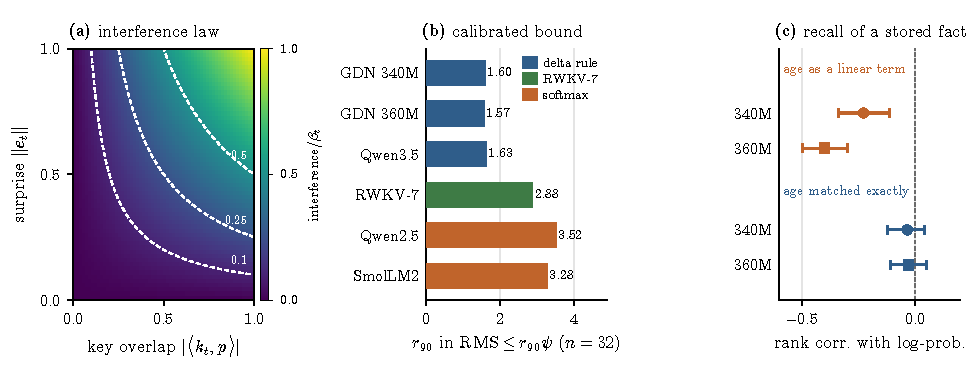
\includegraphics[width=\linewidth]{fig_overview.pdf}
  \caption{Main results. (a) The interference law: a later write disturbs an earlier association by key overlap $\times$ surprise (analytic product; dashed contours of constant interference). (b) The calibrated key-only bound $\mathrm{RMS}\le r_{90}\psi$: the pooled constant $r_{90}$ in six trained models ($n=32$). (c) The bound's task-level test on two Gated DeltaNets: rank correlation of the key-only quantity with the model's recall of a stored fact (``age'' is the distance in tokens between the fact and the query). When age is modelled only linearly the correlation is negative; once age is held fixed exactly, no detectable association remains (95\% bootstrap intervals).}\label{fig:overview}
\end{figure}

\section{Exact laws of interference in a delta-rule state}\label{sec:laws}
The state evolves as $S_t=\alpha_t S_{t-1}(I-\beta_t k_tk_t^\top)+\beta_t v_tk_t^\top$ with unit-norm keys, decay $\alpha_t\in(0,1]$ and write strength $\beta_t\in(0,1]$. The \emph{surprise} is $e_t=\alpha_tS_{t-1}k_t-v_t$.

\begin{lemma}[Interference identity]\label{lem:interf}
For any probe key $p$, $S_tp=\alpha_tS_{t-1}p-\beta_t\langle k_t,p\rangle\,e_t$.
\end{lemma}
\emph{Proof.} Expand $S_tp=\alpha_tS_{t-1}p-\alpha_t\beta_t(S_{t-1}k_t)\langle k_t,p\rangle+\beta_tv_t\langle k_t,p\rangle$ and combine the last two terms. $\square$

\emph{Intuition.} The state stores each pair as the outer product $vk^\top$, and reading with a key $p$ returns $Sp$. A later write whose key overlaps $p$ also changes what the state returns for $p$. The delta rule writes only the \emph{surprise} (what the state failed to predict), so the disturbance is proportional to two things: how much the keys overlap, and how surprising the new value was. Lemma~\ref{lem:interf} makes this exact: a later write therefore disturbs an earlier association by \emph{overlap $\langle k_t,p\rangle$ $\times$ surprise $e_t$}. This is Widrow--Hoff/LMS error correction (and Rescorla--Wagner blocking), and we verified it on the real recurrences of three trained models to a relative residual $\le 1.6\times10^{-6}$ in float32.

Take $\alpha=\beta=1$ and a window of $n$ items with key Gram matrix $G=KK^\top$, $L=\mathrm{tril}(G,-1)$, values $V$. One pass (writing the $n$ pairs once, in order, from the empty state) leaves the error matrix $E=TV$ with $T=L^\top(I+L)^{-1}$, where $E_i=S_nk_i-v_i$ is the error with which item $i$ is recalled. We measure it by $\mathrm{RMS}=\|E\|_F/\sqrt n$; for unit-norm values $\mathrm{RMS}=1$ means the recall is no better than storing nothing. Replacing each value by its own key gives the \emph{key-only} errors $\psi_i=\|(TK)_i\|$ and $\psi_{\mathrm{rms}}=\|TK\|_F/\sqrt n$, which depend on the keys alone. If the keys and values are consistent (some $S^\ast$ fits all pairs) the cumulative surprise obeys $\sum_t\|e_t\|^2\le\|S^\ast\|_F^2=\tr(V^\top G^{-1}V)$ for the minimum-norm $S^\ast$ (a Kaczmarz/Fej\'er argument).

\Needspace{16\baselineskip}
\begin{theorem}[Trace identity for the window error]\label{thm:gain}
Assume the keys of the window are linearly independent, so that $G$ is invertible (this needs $n\le d_k$; in the trained models the window Grams are invertible but ill-conditioned, $\lambda_{\min}\approx0.006$--$0.012$ in Gated DeltaNet 1, which affects how informative the bounds are, not the identities). Let $H=VV^\top$, $M=G^{-1/2}HG^{-1/2}$ (the relative gain of the values over the keys), $B=G^{1/2}T^\top TG^{1/2}$, and $\psi_i=\|(TK)_i\|$ the error of the same pass when the values are the keys themselves. Then
\begin{enumerate}
  \item $n\cdot\mathrm{RMS}^2=\tr(MB)$;
  \item $\mathrm{RMS}\le\sqrt{\lambda_{\max}(M)}\,\psi_{\mathrm{rms}}$;
  \item if $H=g^2G$ (the values' similarity structure is a multiple of the keys') then $\mathrm{RMS}=g\,\psi_{\mathrm{rms}}$ exactly;
  \item for unit-norm rows the key-energy-weighted mean gain equals 1 whatever the values.
\end{enumerate}
\end{theorem}
\emph{Proof.} (1) $\|TV\|_F^2=\tr(THT^\top)=\tr(BM)$. (2) $\tr(MB)\le\lambda_{\max}(M)\tr B$ for PSD $M,B$. (3) $M=g^2I$. (4) $\sum_j\|u_j^\top V\|^2=\|V\|_F^2=n$. $\square$

The identity is an algebraic consequence of $E=TV$. It separates the recall error into a factor computed from the keys alone ($B$, and $\psi$) and a factor that depends on the values ($M$). That separation has three uses here. If the values' structure is proportional to the keys' (item 3), $\psi$ predicts the error up to a constant; when it is only approximately proportional, as measured in the trained models (Section~\ref{sec:measure}), the relation holds approximately and we report the approximation error. This is the basis of the calibrated bound of Section~\ref{sec:measure}. For unit-norm value rows the error obeys the key-only bound $\mathrm{RMS}\le\|T\|_{\mathrm{op}}$, and the \emph{mean gain} $q=\tr(M)/n$ is bounded by $1/\lambda_{\min}(G)$, with equality attainable when the weakest eigenvector of $G$ is flat (Proposition~\ref{prop:nokey}); for other Gram matrices a sharper key-only bound on $q$ may exist. And a budgeted capacity floor shows what a norm budget and a key spectrum allow a linear memory to store (Theorem~\ref{thm:cap}): the number of value directions that can be recalled depends on the spectrum, the alignment of the values with the keys, the norm budget and the error one tolerates, so we give no single capacity number. We also have the permutation expectation of the mean gain under a random pairing of values to keys, conditional on the values' redundancy $\bar h$ (Appendix~\ref{app:theory}). All identities were checked on random instances to machine precision (Figure~\ref{fig:theory}) and Theorem~\ref{thm:gain}'s algebra and the permutation expectation were verified symbolically.

\begin{figure}[t]
  \centering
  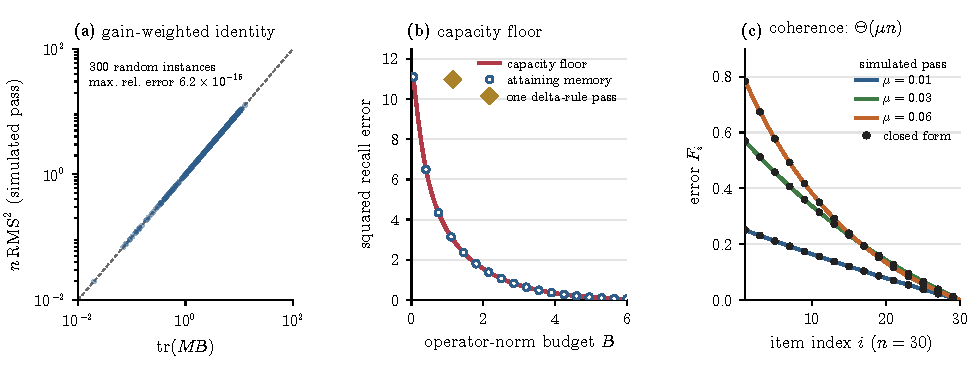
\includegraphics[width=\linewidth]{fig_theory.pdf}
  \caption{Numerical checks of the theory (all computed here from random instances). (a) The gain-weighted identity $n\,\mathrm{RMS}^2=\mathrm{tr}(MB)$ against a simulated delta-rule pass. (b) The budgeted capacity floor $\sum_j(1-B\sqrt{\lambda_j})_+^2$ (Theorem~\ref{thm:cap}; red), the memory that attains it (open circles), and the error of one delta-rule pass at its own operator norm (diamond). (c) Coherence alone: the per-item error of a pass (lines, for three overlap levels $\mu$) against the closed form $(1-\mu)^i-(1-\mu)^n$ of Proposition~\ref{prop:coh} (dots).}\label{fig:theory}
\end{figure}

\section{Measurements on six trained models}\label{sec:measure}
\textbf{Scope: an idealised memory.} We re-implemented the forward pass of Gated DeltaNet \citep{yang2025gdn} (two checkpoints of 340M and 360M parameters) and RWKV-7 \citep{peng2025rwkv7} 0.1B, ran Qwen3.5-0.8B-Base (delta-rule layers) with its native code, and, as controls, two softmax Transformers. For windows of $n\in\{16,32\}$ (and 64) consecutive tokens we build the \emph{idealised} delta-rule memory ($\alpha=\beta=1$, one pass, unit-norm rows, restarted at every window) from a layer's own keys and values and measure its recall error. This is a property of the keys and values of a layer, not of the deployed model's memory: in particular the Transformers' values were never meant to be stored in a delta-rule state, so their numbers describe how well \emph{those keys and values} could be stored, not how well a Transformer recalls. The one measurement on the actual recurrence (below) is therefore the more direct evidence about forgetting in a deployed model.

\textbf{Validation of the re-implementations.} Plausible perplexity does not establish equivalence, so we compare the Gated DeltaNet re-implementation with an independent reference, the gated-delta-rule layer of the HuggingFace \texttt{transformers} library (chunked kernel, the checkpoint's weights mapped into it), on real text. Layer outputs agree to a relative error below $7\times10^{-6}$ in every layer checked; full-model logits agree to at most $1.7\times10^{-4}$ (logits of scale 3--5), with KL divergence below $10^{-6}$, identical perplexity and 100\% top-1 agreement (Appendix~\ref{app:verify}). The RWKV-7 forward pass is compared in the same way with the NumPy reference in the authors' repository (run unmodified, with the checkpoint's weights mapped to its parameter layout): logits agree to at most $4.5\times10^{-5}$ (logits of scale 14--21) in float32 and $2.3\times10^{-13}$ in float64, with identical top-1 predictions and perplexity; Qwen3.5 and the Transformers use library code.

\textbf{Findings.} (i) Trained keys are not incoherent (the largest overlap between two keys is $\mu\approx0.97$) and have effective rank $r_{\mathrm{eff}}=(\tr G)^2/\|G\|_F^2$ of 7--10 against 51 for random keys, which limits how many value directions a given norm budget can store (Theorem~\ref{thm:cap}). (ii) In the idealised memory, the recall error is 0.3--0.6 of the value norm in the Gated DeltaNets for windows of 16--64 tokens, about 0.8 for RWKV-7 and about 1.0 (no better than storing nothing) for the Transformers' keys and values. (iii) In the \emph{actual} recurrence of Gated DeltaNet~1, in its long-memory heads (heads whose decay gate has a half-life of at least 256 tokens; $\approx$26\% of heads), the deviation of a stored association from pure decay caused by later writes (0.12, 0.23, 0.42 after 16, 64, 256 tokens) is about 3 to 20 times the loss from the designed decay gate (0.006, 0.04, 0.16; Figure~\ref{fig:decay}). (iv) The measured gain profile is close to flat when the value branch has no higher rank than the key branch and shares its dominant eigenspace; Theorem~\ref{thm:gain}(3) then holds only approximately (the exact condition $H=g^2G$ is not met), with $\mathrm{RMS}\approx\sqrt q\,\psi_{\mathrm{rms}}$ within 5--7\% in Gated DeltaNet~1 (Appendix~\ref{app:measure}).

\textbf{A calibrated key-only bound.} Define $r_{90}$ as the 90th percentile of $\mathrm{RMS}/\psi_{\mathrm{rms}}$ on calibration text. Then $\mathrm{RMS}\le r_{90}\,\psi_{\mathrm{rms}}$ is an \emph{empirical prediction bound} computed without values (Figure~\ref{fig:r90}); it is a fitted quantile, not a guarantee. Windows, heads and layers of a sequence are not independent, so we report intervals from a bootstrap over the 10--20 source sequences of each model (Table~\ref{tab:r90}): they are narrow ($\le\pm0.1$), and the pooled constants are 1.5--1.7 for the three delta-rule models and 2.7--3.5 for RWKV-7 and the Transformers. The ratio is stable across the five text collections we used (two to four 1024-token sequences each, so five small local collections, not a test of invariance across domains in general). On \heldSeqLo--\heldSeqHi\ new sequences per model, disjoint from the calibration sequences (a post hoc check; Appendix~\ref{app:measure}), the published constants cover \heldCovLo--\heldCovHi\ of the windows against a nominal 0.90, for all six models and both window sizes. The Gated-DeltaNet constants cover only 0.19--0.31 of RWKV-7 windows and 0.00--0.14 of Transformer windows, so the bound must be recalibrated per family; its level tracks the ratio of the value branch's to the key branch's effective rank \emph{within} a model.

\textbf{A gate-aware key-only quantity (post hoc).} The quantity $\psi$ above assumes $\alpha=\beta=1$, whereas the trained models write with their own gates. We therefore ran the recurrence with the model's real decay and write-strength gates but with the values replaced by the keys, so that it depends on keys and gates alone ($D_{\rm gate}$), and compared it with the interference $D_{\rm act}$ measured in the actual recurrence (the quantity of Figure~\ref{fig:decay}) in every layer and head of both Gated DeltaNets, on sixteen 1024-token sequences and delays up to 512 tokens (Appendix~\ref{app:gate}, Figure~\ref{fig:gate}). Within a head, after removing the decay gate, $D_{\rm gate}$ ranks the positions by interference with a rank correlation of \gatePartLo--\gatePartHi\ in long-memory heads, over all delays and both models; the gate-free quantity gives \freePartLo--\freePartHi, falling to about zero at 512 tokens, and permuting the keys while keeping the gates gives \shufPartLo--\shufPartHi, so the key geometry carries a real share of the signal and the gates the rest. This analysis is post hoc and covers two models of one family; whether the same quantity predicts recall is the question of Section~\ref{sec:task}.

\textbf{Reading Section~\ref{sec:measure}.} The idealised-memory numbers say how well a layer's own keys and values \emph{could} be stored in a one-pass delta-rule memory; the key-only quantity $\psi$ tracks that error up to a constant per model family; and the one actual-recurrence measurement shows that later writes, not the decay gate, dominate what is lost in the long-memory heads of one model. None of this yet says that $\psi$ predicts what a model recalls on a task, which is the question of Section~\ref{sec:task}.

\begin{figure}[t]
  \centering
  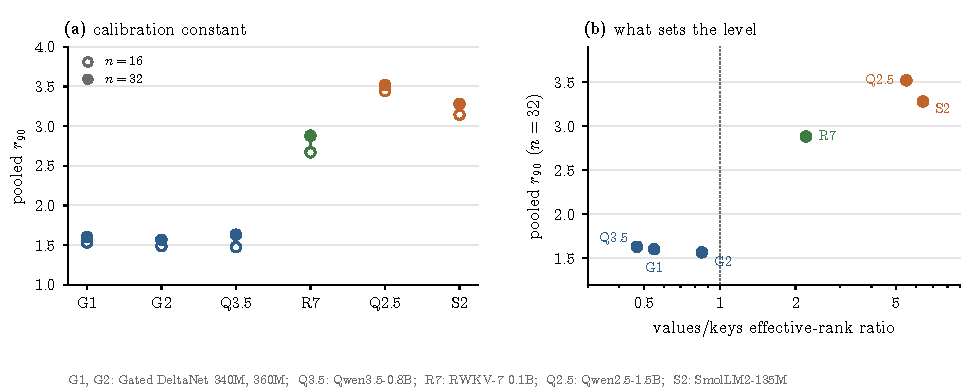
\includegraphics[width=\linewidth]{fig_measure.pdf}
  \caption{The measurement study. (a) Pooled calibrated constant $r_{90}$ by model and window size: the three delta-rule models cluster at 1.5--1.7, RWKV-7 and the two Transformers sit at 2.7--3.5. (b) The level of $r_{90}$ against the ratio of the effective rank of the values to that of the keys (six points: a pattern, not a law).}\label{fig:r90}
\end{figure}

\begin{figure}[t]
  \centering
  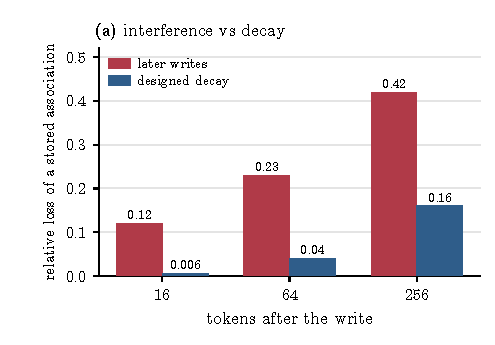
\includegraphics{fig_decay.pdf}
  \caption{Interference against designed decay in the \emph{actual} recurrence of Gated DeltaNet~1 (long-memory heads, real $\alpha_t$, $\beta_t$ and values): relative loss of a stored association after 16, 64 and 256 tokens. The measured deviation from pure decay is about 3 to 20 times the loss from the decay gate.}\label{fig:decay}
\end{figure}

\section{A pre-registered task-level test}\label{sec:task}
\textbf{Question.} Does the same key-only quantity, computed from the model's own keys on a prompt, predict whether the \emph{model} recalls a stored fact on a downstream task, beyond simple baselines? The expectation was simple: if $\psi$ is large for a fact, the idealised memory would find it hard to store, so the model should recall it less often. The protocol was written before any bound was computed (Appendix~\ref{app:task}).

\textbf{Task.} Each prompt lists $n\in\{4,8,16,24\}$ facts ``$\langle$Key$\rangle$ is $\langle$value$\rangle$.'' (single-token names and common words, all distinct) and queries one; 150 prompts per load, 600 per model, on Gated DeltaNet 340M (primary) and 360M (replication). Strict top-1 over the vocabulary is dominated by the format prior, so the outcome is \emph{forced-choice recall} (the true value ranked first among the $n$ stated values; chance $1/n$), a change recorded after an accuracy-only pilot and before any bound was computed. The predictor $P_1$ is $\psi_i=\|(TK)_i\|$ averaged over the queried fact's three tokens and over the long-memory heads (median decay half-life $\ge256$ tokens on calibration prompts: 21/96 and 20/84 heads). Prompts are split 50/50 by prompt.

\textbf{Pre-registered criterion (H1).} Adding $P_1$ to age (tokens between the fact and the query) and load raises test AUC by $\ge0.03$ with a bootstrap interval excluding 0, on the primary model and replicated in the second.

\begin{table}[t]
  \caption{Task-level test. Forced-choice accuracy at $n=4/8/16/24$ (chance $.25/.125/.06/.04$), test AUC of the pre-registered baseline B3 (age and one-hot load) with and without $P_1$, and the pre-registered comparison $\Delta$ with its 95\% bootstrap interval.}\label{tab:task}
  \centering\small\setlength{\tabcolsep}{4pt}
  \begin{tabular}{lcccc}
\toprule
Model & accuracy at $n=4/8/16/24$ & AUC age$+$load & AUC $+P_1$ & $\Delta$ (95\% CI) \\
\midrule
GDN 340M (primary) & .34/.25/.17/.17 & .644 & .644 & $\pm$.000 ($-$.041, $+$.038) \\
GDN 360M (replic.) & .44/.46/.40/.34 & .575 & .693 & $+$.118 ($+$.056, $+$.182) \\
\bottomrule
\end{tabular}

\end{table}

\textbf{Verdict.} The pre-registered claim is \emph{not confirmed}: the primary model fails and the replication passes only in the pooled test. \textbf{Exploratory follow-up (post hoc).} Within a load, $P_1$ correlates 0.87--0.98 with age ($\psi$ is larger for facts written earlier). Age is a deterministic function of the queried position for a given load, so prompts with the same load \emph{and} the same queried position (48 cells) have identical age. Within those cells the rank correlation of $P_1$ with the true value's log-probability among the candidates is $-0.035$ ($-0.121,+0.041$) for the 340M model and $-0.030$ ($-0.108,+0.049$) for the 360M model, against shuffled-$\psi$ nulls of $0.000$ and $-0.005$ (Figure~\ref{fig:task}). The pooled gain in the 360M model is therefore explained by the pre-registered baseline modelling age only linearly. In this setting we find no detectable incremental association between the key-only quantity and recall beyond the distance to the query. What the three analyses exclude is different and we keep it apart. (a) Under exact age control the within-cell rank correlations exclude $|\rho|$ beyond about $0.12$. (b) The pre-registered pooled comparison (age modelled linearly) gives a primary-model gain of $0.000$ with interval $(-0.041,+0.038)$, excluding gains above about $0.04$ AUC in that model; the replication's pooled gain of $+0.118$ is explained by the linear age baseline. (c) A post-hoc held-out comparison with a flexible categorical age adjustment (a fixed effect for every (load, queried position) cell, fitted on the calibration prompts; Appendix~\ref{app:task}) gives a gain of $\flexDa$ ($\flexLoa$, $\flexHia$) in the 340M model and $\flexDb$ ($\flexLob$, $\flexHib$) in the 360M model; the upper endpoints of these intervals are below $0.02$ and $0.01$ AUC for these fitted comparisons (Table~\ref{tab:taskresults}). The intervals come from resampling test prompts with the fitted models held fixed, so they do not exclude other predictors, interactions or fitting procedures, nor smaller effects, other prompt formats, longer contexts or other models.

\begin{table}[ht]
  \caption{Task-level results side by side (95\% bootstrap intervals). $\Delta$AUC is the held-out AUC gain from adding $P_1$: the pre-registered comparison models age linearly; the categorical-age comparison (a fixed effect for every load and queried position) and the within-cell rank correlation are post hoc.}\label{tab:taskresults}
  \centering\setlength{\tabcolsep}{5pt}
  \begin{tabular}{lccc}
\toprule
model & pre-registered $\Delta$AUC & categorical-age $\Delta$AUC & within-cell $\rho$ \\
\midrule
GDN 340M & $\pm$.000 ($-$.041, $+$.038) & $+$.001 ($-$.017, $+$.017) & $-$.035 ($-$.121, $+$.041) \\
GDN 360M & $+$.118 ($+$.056, $+$.182) & $\pm$.000 ($-$.006, $+$.007) & $-$.030 ($-$.108, $+$.049) \\
\bottomrule
\end{tabular}

\end{table}

\begin{figure}[t]
  \centering
  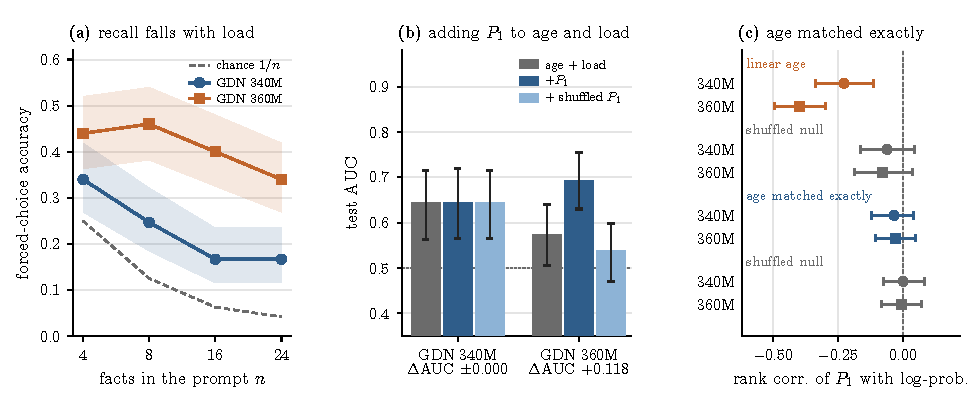
\includegraphics[width=\linewidth]{fig_task.pdf}
  \caption{Task-level test. (a) Forced-choice recall against load for the two Gated-DeltaNet models (bands: 95\% Wilson intervals; chance dashed). (b) Test AUC of the pre-registered baseline B3 with $P_1$ and with a shuffled $P_1$ (error bars: bootstrap 95\% intervals); $\Delta$AUC is the pre-registered comparison. (c) Rank correlation of $P_1$ with the true value's log-probability among the candidates: the estimates that control age only linearly are significantly negative, with age and load fixed exactly (within-cell) they are indistinguishable from 0, and a shuffled $P_1$ gives the null in both settings (95\% intervals).}\label{fig:task}
\end{figure}

\textbf{Caveats.} Small models with weak recall (forced-choice accuracy 0.17--0.46); prompts of at most about 100 tokens, shorter than the state ($d_k=256$) can saturate, so interference may not be the binding constraint; $\psi$ uses $\alpha=\beta=1$ and a whole-prefix window beyond the 16--64-token calibration range; one prompt format. A gate-aware predictor, tested post hoc (Appendix~\ref{app:gatetask}), adds no detectable information either: its gain over the flexible age baseline is $\gFlexDa$ ($\gFlexLoa$, $\gFlexHia$) in the 340M model and $\gFlexDb$ ($\gFlexLob$, $\gFlexHib$) in the 360M model. A larger model (1.3B, post hoc extension under a protocol fixed beforehand; Appendix~\ref{app:scale}) recalls no better in this format (forced-choice accuracy \scAccFour, \scAccEight, \scAccSixteen, \scAccTwentyFour\ at $n=4,8,16,24$) and again gives no gain above the criterion: $P_1$ and $P_{1g}$ add $\scGfreeFlexD$ ($\scGfreeFlexLo$, $\scGfreeFlexHi$) and $\scGawareFlexD$ ($\scGawareFlexLo$, $\scGawareFlexHi$) AUC over the flexible age baseline; by the verdict rule fixed in advance the outcome is ``mixed'' because one gate-aware within-cell interval narrowly excludes zero, in the direction opposite to the hypothesis. Longer contexts and models with stronger recall were not tested. A first analysis run was invalid because the extraction stored mean log-decay rather than the median half-life the protocol specifies; the head groups were then computed from calibration prompts only, and this is logged as a deviation.

\section{A training-time experiment and its replication}\label{sec:lever}
\textbf{Motivation.} The theory says the error depends on the key geometry, in particular on how many independent key directions there are (the effective rank). A regulariser that spreads the keys out should therefore help, and this experiment checks it in a small trained model.

\textbf{Task.} Multi-query associative recall with distractors: a sequence has $n$ (key, value) token pairs, then $L$ filler tokens, then the $n$ keys again in random order, and the model must output each key's value. Training uses $n\in[4,32]$, $L\in[0,96]$; evaluation $n\in\{8,16,24,32\}$, $L\in\{0,32,96\}$. The task is load-sensitive and, over the distractor lengths tested, insensitive to distractor length: across the \mqNLearned\ of \mqNRuns\ runs whose mean recall exceeds 0.5, accuracy at $L=0$ and $L=96$ differs by at most \mqMaxGap, while accuracy falls with $n$, the number of items competing for the state (this does not isolate capacity from other limits).

\textbf{Model and regularisers.} A 113k-parameter two-layer gated delta-rule model (2 heads, $d_k=d_v=32$; chunked reference implementation, checked against a step-by-step loop to $7\times10^{-8}$), AdamW, 3000 steps. Three \emph{task-agnostic} regularisers computed from the layer's own keys and values on the first 16 positions of every sequence, chosen from the theory before any run with one untuned weight each: \emph{key decorrelation} (penalise the mean squared off-diagonal key cosine, raising the keys' effective rank), \emph{Gram matching} (push the relative gain towards 1, $M\to I$) and \emph{rank matching} (penalise value rank above key rank).

\begin{table}[t]
  \caption{Mean recall accuracy (over $L$) by $n$; seeds 0--11, twelve for each of the four learners.}\label{tab:lever}
  \centering\small\setlength{\tabcolsep}{4pt}
  \begin{tabular}{lccccccc}
\toprule
learner & seeds & $n{=}8$ & 16 & 24 & 32 & mean & SD across seeds \\
\midrule
baseline & 12 & .879 & .834 & .783 & .721 & .804 & .294 \\
\textbf{key decorrelation} & 12 & \textbf{.997} & \textbf{.993} & \textbf{.969} & \textbf{.916} & \textbf{.969} & \textbf{.019} \\
Gram matching & 12 & .837 & .795 & .741 & .676 & .762 & .323 \\
rank matching & 12 & .830 & .759 & .694 & .622 & .726 & .299 \\
\bottomrule
\end{tabular}

\end{table}

\begin{figure}[t]
  \centering
  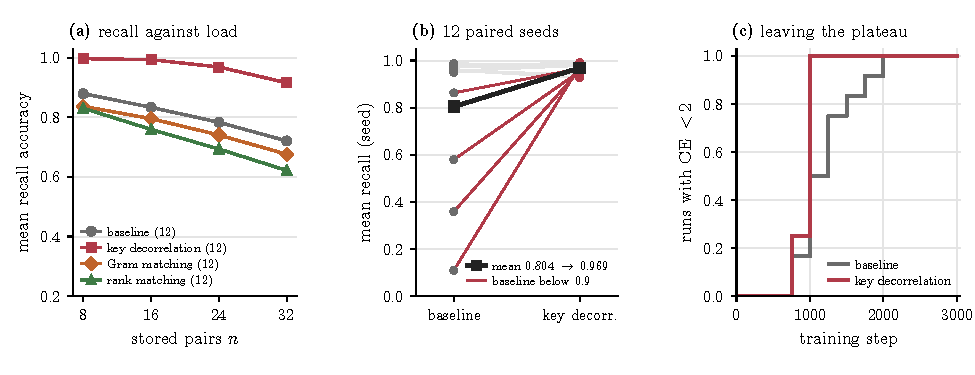
\includegraphics[width=\linewidth]{fig_lever.pdf}
  \caption{The training-time lever, first twelve seeds. (a) Recall against the number of stored pairs for the four learners (number of seeds in brackets). (b) Paired seeds: baseline against key decorrelation (red lines: the \mqFailBase\ baseline seeds below 0.9 mean recall; black: mean). (c) Fraction of runs whose training cross-entropy has left the chance plateau (below 2) by each step: key decorrelation leaves it by step 1000 in 12 of 12 runs, the baseline in 6 of 12.}\label{fig:lever}
\end{figure}

\textbf{Results, seeds 0--11.} Key decorrelation versus baseline (same seed): mean paired difference $\mqDiff$ (bootstrap 95\% CI $[\mqCiLo,\mqCiHi]$), \mqHigher\ of \mqN\ seeds higher, exact sign-flip $p=\mqSF$, exact Wilcoxon $p=\mqWil$; three regularisers were compared, and after a Holm correction over them the sign-flip $p$ for decorrelation is $\mqHolm$. The effect was carried by the baseline's failures to learn: \mqFailBase\ of the \mqN\ baseline seeds stayed below 0.9 mean recall, against \mqFailDec\ decorrelated runs (Fisher $p=\mqFisher$); their gains are \mqFailGains, and in the other \mqNRest\ seeds the gain is $\mqGainRest$. Decorrelated runs leave the chance plateau by step 1000 in 12/12 runs (baseline 6/12). The geometric account of these seeds (Appendix~\ref{app:lever}): the baseline's second layer collapses to a key rank of 2.0 with a non-flat gain ($q=14.9$, $\mathrm{RMS}/\psi=2.16$), the regime of RWKV-7 and the Transformers in Section~\ref{sec:measure}; decorrelation holds that layer's key rank at 11.5 ($q=1.39$). Gram matching drives $\mathrm{RMS}/\psi$ to \gramRmsLo--\gramRmsHi\ without helping, by shrinking both ranks to \gramRankLo--\gramRankHi: a flat gain is cheap to obtain by collapse, and informative only when the ranks are healthy.

\textbf{Replication, seeds 12--23.} We then ran twelve new seeds of the baseline and of key decorrelation with the identical configuration, under a protocol fixed beforehand (Appendix~\ref{app:leverrep}), and completed Gram matching and rank matching to twelve seeds each. \textbf{The effect did not replicate}: the paired difference is $\repDiff$ ($[\repCiLo,\repCiHi]$), \repHigher\ of 12 seeds higher, exact sign-flip $p=\repSF$, Wilcoxon $p=\repWil$; mean recall is \repBaseMean\ for the baseline and \repDecMean\ for decorrelation, and \repFailBase\ baseline and \repFailDec\ decorrelated runs stayed below 0.9. Pooled over all 24 seeds the difference is $\poolDiff$ ($[\poolCiLo,\poolCiHi]$, $p=\poolSF$), with \poolFailBase\ baseline and \poolFailDec\ decorrelated runs below 0.9 of 24 (Fisher $p=\poolFisher$). Whether a run learns depends on the seed at least as much as on the regulariser. Decorrelation does what it is designed to do, raising the layer-1 key effective rank (median \mqNewKeyDec\ against \mqNewKeyBase\ in the new runs), but accuracy no longer tracks the key rank there (Spearman $\mqNewSp$ over the 24 new runs, against $\mqSpKey$ over the 48 runs of seeds 0--11). With twelve seeds each, Gram matching and rank matching differ from the baseline by $\matchDiff$ ($p=\matchSF$) and $\rankDiff$ ($p=\rankSF$): no detectable effect, so the earlier impression that they were worse, from six and three seeds, is not supported. We conclude that the evidence does not establish that key decorrelation makes training of this model more reliable. \textbf{Caveats:} one task, one small model, one untuned weight per regulariser; training in this setting is high-variance (\poolFailBase\ of 24 baseline runs stay below 0.9 mean recall).

\section{Related work and what is new}\label{sec:related}
We ran a systematic search (arXiv and OpenAlex; 17 pre-specified search strings, two post-hoc amendments, citation chasing; 4{,}017 + 2{,}094 records retrieved, 327 included; protocol and data released; end-to-end recall 76\% on a 33-paper reference set; two databases only, one automated reviewer, mostly abstract-level screening; Appendix~\ref{app:review}). The nearest prior work for each claim:
\begin{itemize}
  \item \textbf{Delta-rule law and capacity.} The update is Widrow--Hoff/LMS and Rescorla--Wagner error correction \citep{widrow1960adaptive,rescorla1972theory}; delta-rule capacity was studied analytically in 1989 \citep{prados1989capacity}; recent work derives delta-rule steps from online regression and Kaczmarz projection \citep{wang2025testtime,liu2025longhorn}, treats DeltaNet as test-time regression \citep{yang2024deltanet,yang2025gdn,sun2024ttt,behrouz2025titans} and analyses interference in fixed-state recurrences. Our Lemma~\ref{lem:interf} is a restatement.
  \item \textbf{Zero-interference update, memory and frontier (supplement).} (Used only in the supplement.) The update of Theorem~\ref{thm:frontier}(a) is ORFit \citep{min2022orfit}, which also truncates the stored basis by PCA; Grassmannian packing gives memory lower bounds for streaming regression \citep{dagan2019space}; covering numbers are classical \citep{szarek1998metric,pajor1998metric}; Pareto and stability/plasticity analyses of projection methods exist \citep{zhao2023rethinking}; \citet{chen2022memory} and \citet{knoblauch2020optimal} give memory lower bounds for general learners.
  \item \textbf{Projection and SSM continual learning.} Projection methods restrict each update to the complement of a stored subspace of old gradients or activations: GPM \citep{saha2021gradient}, OGD \citep{farajtabar2020orthogonal}, Adam-NSCL \citep{wang2021training}, Mamba-CL \citep{cheng2024mamba} and Inf-SSM \citep{lee2025exemplar}; our layerwise argument is theirs with a frozen recurrence.
  \item \textbf{Closest empirical work (full text read).} \citet{lee2026how} apply causal interventions (state and write swaps, write-key alignment) to pretrained GLA and Gated DeltaNet models up to 1.3B and to hybrids, on the actual recurrence, and find that distractor writes aligned with a target key lower its margin and that load costs far more than distance; they report no separation of key geometry from value gain, no calibrated bound and no predictor of recall. \citet{boesch2026anatomy} study matched-state recurrences at toy scale (one layer, $d=32$), report that failures to learn are seed-dependent (``lock-in'' rates) and that a distance curriculum raises them from 1/10 to 7/10; they measure behaviour only, not the state. Our interference measurement is convergent with the first and our training result with the second; neither overlaps with the trace-identity separation, the calibration across six models or the pre-registered downstream test.
  \item \textbf{Forgetting theory in linear models.} \citet{evron2022catastrophic} and follow-ups; \citet{lin2023theory}.
\end{itemize}
\textbf{What we found no counterpart for} (at abstract level, plus the full text of the two papers above) is the separation of key geometry from value gain used as a measurement tool: the idealised-memory measurements and the calibrated key-only bound with its transfer limits across six models; the discrepancy between the bound's predictiveness for the idealised memory and its absence of detectable incremental association with downstream recall after adjusting for age; and the negative and comparative results on small diagonal SSMs. The interference measurement in the actual recurrence and the seed-dependence of training failures have close counterparts (above); the trace identity is a short algebraic consequence of the single-pass error operator and we claim it only for its use here.

\section{Using the diagnostic, and lessons from the negative results}\label{sec:use}
\subsection{Using the diagnostic}
\textbf{A recipe.} (1) For a layer and a window of $n$ tokens, take the unit-normalised keys and form the Gram matrix $G$; its effective rank $r_{\rm eff}$ and its conditioning $\lambda_{\min}(G)$ say how many value directions the keys can hold (Theorem~\ref{thm:cap}; Table~\ref{tab:notation}). (2) Compute $\psi$ with one triangular solve ($T=L^\top(I+L)^{-1}$; the code is in \texttt{flatlib.py} of the repository). (3) Read the bound $\mathrm{RMS}\le r_{90}\psi$ with the constant of the model's family (1.5--1.7 for the delta-rule models, 2.7--3.5 for RWKV-7 and the Transformers) and recalibrate it on a few sequences for a new family; on new text from the same sources the published constants cover \heldCovLo--\heldCovHi\ of the windows. (4) Check the regime: the ratio of the values' to the keys' effective rank orders the models by the level of the constant (Section~\ref{sec:measure}). (5) To describe interference in a deployed model, run the recurrence with the real gates and the values replaced by the keys ($D_{\rm gate}$, Appendix~\ref{app:gate}); within a head, after removing the decay gate, it ranks the positions by interference with a rank correlation of \gatePartLo--\gatePartHi. (6) Do not read any of these as a predictor of recall: in the regimes we tested, none is one (Section~\ref{sec:task}).

\begin{table}[H]
  \caption{What the diagnostic can and cannot tell you, as tested here.}\label{tab:use}
  \centering\scriptsize\setlength{\tabcolsep}{4pt}
  \begin{tabular}{>{\raggedright\arraybackslash}p{7.6cm}>{\raggedright\arraybackslash}p{7.6cm}}
    \toprule
    can & cannot \\
    \midrule
    bound the idealised memory's error from the keys alone, with a family-calibrated constant & predict whether a model recalls a stored fact beyond age and load \\
    flag key-rank collapse and ill-conditioned windows & certify anything across model families without recalibration \\
    compare key geometry across layers, heads and models & show that decorrelating keys makes training more reliable \\
    rank the positions that suffer interference within a head, using the real gates (gate-aware version) & say anything about Transformer recall (the Transformer numbers describe key geometry only) \\
    \bottomrule
  \end{tabular}
\end{table}

\subsection{Lessons from the negative results}
\textbf{Control the confound exactly.} In the pre-registered test the age of a fact (tokens between the fact and the query) is nearly collinear with $P_1$ (rank correlation 0.87--0.98 within a load). A pooled gain of $+0.118$ AUC in the 360M model, over a baseline that modelled age only linearly, disappeared ($\flexDb$) once age was controlled exactly with a fixed effect for every (load, queried position) cell.

\textbf{Report null controls and their spread.} In the 1.3B model the shuffled predictors give within-cell correlations of $\scGfreeshIn$ and $\scGawareshIn$ with intervals that exclude zero, and six of the 24 intervals in that table exclude zero; one interval that excludes zero is weak evidence when a table holds dozens that are uncorrected.

\textbf{Replicate before believing, and correct for multiplicity.} The key-decorrelation gain over twelve seeds ($p=\mqSF$) is $\mqHolm$ after a Holm correction over the three regularisers tested, and it did not replicate over twelve new seeds ($p=\repSF$). Training of the small model is high-variance (\poolFailBase\ of 24 baseline runs stay below 0.9 mean recall), so a dozen seeds can mislead.

\textbf{Say which memory is measured.} Results for the idealised memory do not transfer to the deployed recurrence without the gates: the gate-free quantity's correlation with the interference in the actual recurrence falls to about zero at delays of 512 tokens, while the gate-aware one keeps \gatePartLo--\gatePartHi. Pre-registration made these nulls interpretable: the criteria, the analyses and the deviations, including an implementation error that was found and logged, were fixed or recorded beforehand.

\section{Conclusion}\label{sec:concl}
In a delta-rule memory a later write disturbs an earlier association in proportion to key overlap times surprise, and the error of a one-pass memory splits into a part set by the keys and a part set by how the values align with them. This paper offers exact laws for that split; a calibrated, value-free diagnostic, with constants of 1.5--1.7 for the delta-rule models and 2.7--3.5 for RWKV-7 and the two Transformers, stable across five text collections and covering \heldCovLo--\heldCovHi\ of the windows of new text but not transferable between families; and a gate-aware version that tracks the interference measured in the actual recurrence of two Gated DeltaNets. It also reports what the diagnostic does not do. In a pre-registered test on two Gated DeltaNets it did not predict recall of a stored fact once the distance to the query was accounted for, and neither did gate-aware predictors or a 1.3B model, tested under a protocol fixed beforehand, although recall in this format is weak in all three; and a key-decorrelation regulariser that improved a small model's training over a first set of seeds did not do so over twelve new ones. We read this as: key geometry is a useful measurement tool for what a delta-rule memory could store and how it is overwritten, not yet a predictor of what a model recalls. Whether it becomes one in longer contexts or in models with stronger recall is the open question.

\section{Limitations}\label{sec:limits}
\begin{enumerate}
  \item The measurement study analyses an \emph{idealised} one-pass memory ($\alpha=\beta=1$, unit-norm rows, windows of at most 64 tokens), not the deployed model's memory; the Transformer numbers say nothing about Transformer recall. The actual recurrence is measured in two models of one family (Figure~\ref{fig:decay}; the gate-aware analysis of Appendix~\ref{app:gate} is post hoc, on 1024-token sequences from two domains); the gate-aware task-level analysis uses prompts of at most about 100 tokens, so its reach to longer contexts is untested.
  \item The calibrated bound is empirical: a fitted 90th percentile from 10--20 sequences per model, with five small local text collections, not a guarantee and not evidence of invariance across domains. It does not carry over between families. On \heldSeqLo--\heldSeqHi\ new sequences per model its published constants cover \heldCovLo--\heldCovHi\ of the windows (Appendix~\ref{app:measure}), which supports stability within a family on similar local text, not invariance across domains.
  \item The task-level test (Section~\ref{sec:task}) is a null result in one setting: three Gated DeltaNets (340M to 1.3B) with weak recall and short prompts. It does not show that the key-only quantity carries no information in general, and the flexible-age and gate-aware comparisons are post hoc.
  \item The capacity statements are floors for linear memories at a stated norm budget and error tolerance; low effective rank alone does not fix a capacity.
  \item The training-time lever (Section~\ref{sec:lever}) is one task and one small model; its effect in the first twelve seeds (uncorrected $p=\mqSF$, Holm-adjusted $\mqHolm$) did not replicate in twelve new seeds.
  \item Six checkpoints (three of one family). The Gated DeltaNet re-implementations are validated against an independent reference layer (not the original authors' kernels); the RWKV-7 re-implementation against the NumPy reference in the authors' repository (neither against the authors' GPU kernels).
  \item The weight-space experiments (supplement) use small real-diagonal SSMs, synthetic and MNIST streams, five seeds and one optimiser; they are not a ranking of published methods.
  \item The literature search is systematic but not exhaustive; the amendments were made after seeing results.
\end{enumerate}

\section*{Reproducibility}
Code, protocols (including the pre-registration of Section~\ref{sec:task} with its deviations), raw results, the validation scripts and the literature-review data are in the accompanying repository, \url{https://github.com/excyst-cerebral/delta-rule-key-geometry}. Model checkpoints were obtained from the Hugging Face Hub; no repository code from the checkpoints was executed.

\bibliographystyle{unsrtnat}
\bibliography{references}

\appendix
\clearpage
\section*{Appendix}
\addcontentsline{toc}{section}{Appendix}
The appendix collects (A) the full theory of the delta-rule state, (B) the measurement-study details, (C) the training-time experiment, (D) the task-level test, (E) the systematic literature review and (F) verification and reproducibility; the supplement on continual learning in the weights follows as (G) a summary, (H) the weight-space theory and (I) the experimental details. Statements are numbered consecutively with the main text.

%==============================================================================
\section{Theory of the delta-rule state}\label{app:theory}
\subsection{Definitions: replay, anchor, pure learner; three kinds of statement}
A \emph{learner} processes a task stream. We call \emph{replay} any learner that stores or regenerates examples of earlier tasks; an \emph{anchor} any learner that stores parameters or a derived object (importance matrix, subspace basis, per-task modules) computed from earlier tasks; and a \emph{pure} learner one that does neither: its state after a task is a function of the previous parameters and the current task's data only. Optimiser moments, weight decay and fixed random embeddings are treated as part of the architecture; a different convention would move some methods across the line. Under these definitions the original question asks for guarantees from a pure learner. Orthogonal-projection methods (OGD, GPM, Mamba-CL), EWC, replay and freezing all store information about the past.

We use three kinds of statement about forgetting. An \emph{exact law} is an identity that holds for every instance (Lemma~\ref{lem:interf}). A \emph{deterministic bound} is an inequality that holds under stated hypotheses on keys and values. A \emph{calibrated bound} is an inequality $\mathrm{RMS}\le r\,\psi$ whose constant $r$ is estimated from other data and which holds with an empirical coverage; it is a statistical statement about a model family, not a guarantee for an arbitrary instance.

\subsection{Exact laws}
Throughout, keys have unit norm; statements that use $G^{-1}$ or $G^{-1/2}$ assume the window's keys are linearly independent ($n\le d_k$ and $G$ invertible). The recurrence of the main text is $S_t=\alpha_tS_{t-1}(I-\beta_tk_tk_t^\top)+\beta_tv_tk_t^\top$.

\begin{theorem}[Retention bound]\label{thm:retention}
If item $i$ is written at time $s$, then
\[
\Big\|S_Tk_i-\Big(\prod_{t>s}\alpha_t\Big)S_sk_i\Big\|\;\le\;\sum_{t=s+1}^{T}\beta_t\,|\langle k_t,k_i\rangle|\,\|e_t\|\;\le\;\mu\sum_t\beta_t\|e_t\|,
\]
where $\mu$ is the maximal key coherence.
\end{theorem}
\begin{proof}
Unrolling Lemma~\ref{lem:interf}: $r_T=(\prod\alpha)r_s-\sum_t(\prod_{u>t}\alpha_u)\beta_t\langle k_t,k_i\rangle e_t$ with $r_t=S_tk_i$; take norms.
\end{proof}
Forgetting therefore splits into \emph{designed decay} (the $\alpha$ schedule) and \emph{interference} (at most $\mu\times$ the cumulative surprise). Under orthogonal keys interference is exactly zero.

\begin{proposition}[Single-pass error operator, $\alpha=\beta=1$]\label{prop:errop}
With $W=(I+L)^{-1}V$ (rows $w_t=-e_t$), the error matrix of one pass is $E_i=S_nk_i-v_i$, $E=L^\top W=TV$ with $T=L^\top(I+L)^{-1}$, and $F_i=\|E_i\|=\|\sum_{j>i}G_{ij}w_j\|$. The values enter only through $H=VV^\top$, since $EE^\top=THT^\top$.
\end{proposition}
\begin{proof}
Write $S_t=\sum_{j\le t}w_jk_j^\top$ with $w_j=v_j-S_{j-1}k_j$. Then $(I+L)W=V$, the predictions are $GW$, and $G=I+L+L^\top$; hence $E=GW-V=(L+L^\top)W+W-V=L^\top W+(I+L)W-V=L^\top W$.
\end{proof}

\begin{theorem}[Bounded cumulative surprise]\label{thm:surprise}
For $\alpha=\beta=1$, a jointly consistent window (some $S^\ast$ fits every pair; e.g.\ independent keys) and any write order (repeats allowed), $\|S_t-S^\ast\|_F$ is non-increasing and $\sum_t\|e_t\|^2\le\|S^\ast\|_F^2$. For the minimum-norm interpolant $S^\ast=V^\top G^{-1}K$ (which needs $G$ invertible), $\|S^\ast\|_F^2=\tr(V^\top G^{-1}V)$, and this is the tightest choice.
\end{theorem}
\begin{proof}
With $\alpha=\beta=1$ and unit keys, $S_t-S^\ast=(S_{t-1}-S^\ast)(I-k_tk_t^\top)$ because $S^\ast k_t=v_t$. Writing $D=S_{t-1}-S^\ast$, $\|D(I-kk^\top)\|_F^2=\|D\|_F^2-\|Dk\|^2$ and $Dk=S_{t-1}k_t-v_t=e_t$. Summing from $S_0=0$ gives $\sum\|e_t\|^2\le\|S^\ast\|_F^2$. For $S^\ast=V^\top G^{-1}K$: $\|S^\ast\|_F^2=\tr(V^\top G^{-1}KK^\top G^{-1}V)=\tr(V^\top G^{-1}V)$.
\end{proof}
(This is the Kaczmarz/Fej\'er projection argument: one step is the orthogonal projection of the state onto $\{S:Sk_t=v_t\}$, which contains $S^\ast$. The identities in this theorem were also verified symbolically in the Wolfram Language.)

\begin{proof}[Complete proof of Theorem~\ref{thm:gain}]
Define the mean gain $q=\tr(M)/n=\tr(V^\top G^{-1}V)/n=\|S^\ast\|_F^2/n$ and $\psi_{\mathrm{rms}}^2=n^{-1}\|TK\|_F^2=n^{-1}\tr B$. (1) $\|TV\|_F^2=\tr(THT^\top)=\tr(T G^{1/2}MG^{1/2}T^\top)=\tr(BM)$. (2) For PSD $M,B$: $\tr(MB)\le\lambda_{\max}(M)\tr B$ and $\tr(MB)\le\|B\|_{\mathrm{op}}\tr M$; hence $\mathrm{RMS}\le\sqrt{\lambda_{\max}(M)}\,\psi_{\mathrm{rms}}$ and $\mathrm{RMS}\le\|TK\|_{\mathrm{op}}\sqrt q$. (3) If $H=g^2G$ then $M=g^2I$, so $\tr(MB)=g^2\tr B$, $F_i=g\psi_i$ for every item, $q=g^2$ and $\mathrm{RMS}=\sqrt q\,\psi_{\mathrm{rms}}$. (4) Let $G=\sum_j\lambda_ju_ju_j^\top$ and $\kappa_j=\|u_j^\top V\|^2/\lambda_j$. For unit-norm rows $\sum_j\|u_j^\top V\|^2=\|V\|_F^2=n$ and $\sum_j\lambda_j=\tr G=n$, so $\sum_j\lambda_j\kappa_j=n=\sum_j\lambda_j$: the key-energy-weighted mean gain is exactly 1 whatever the values.
\end{proof}

\begin{proposition}[Permutation expectation of the mean gain, conditional on value redundancy]\label{prop:expq}
For a uniformly random permutation $\pi$ of the rows of any fixed unit-row $V$,
\[
\E_\pi[q]=\frac{\tr(G^{-1})(1-\bar h)+\bar h\,\mathbf 1^\top G^{-1}\mathbf 1}{n},\qquad \bar h=\frac{\|\sum_iv_i\|^2-n}{n(n-1)}.
\]
\end{proposition}
\begin{proof}
$q=n^{-1}\sum_{a,b}(G^{-1})_{ab}\langle v_{\pi(a)},v_{\pi(b)}\rangle$. The diagonal terms equal $(G^{-1})_{aa}$; each off-diagonal pair has expected cosine $\bar h$, the mean pairwise cosine of the values. Collect terms.
\end{proof}
$\bar h$ is the values' redundancy; everything else is a function of the keys. (We verified the formula against the exact average over all $n!$ permutations with symbolic $G^{-1}$ and symbolic unit-diagonal value Gram matrix for $n=3,4,5$, residual $0$.)

\subsection{Limits: what cannot be guaranteed}
\begin{theorem}[Budgeted capacity floor]\label{thm:cap}
Let $G=\sum_j\lambda_ju_ju_j^\top$ with $K=\sum_j\sqrt{\lambda_j}u_jy_j^\top$. For any index set $J$ and orthonormal $\{w_j\}_{j\in J}\subset\R^{d_v}$ let $V=\sum_{j\in J}u_jw_j^\top$. For every linear memory $S$ with $\|S\|_{\mathrm{op}}\le B$,
\[
\|KS^\top-V\|_F^2\;\ge\;\sum_{j\in J}\big(1-B\sqrt{\lambda_j}\big)_+^2,
\]
and some $S$ with $\|S\|_{\mathrm{op}}\le B$ attains equality. The delta rule satisfies $\|S_t\|_{\mathrm{op}}\le\|V_{\le t}\|_F$ automatically (Lemma~\ref{lem:budget}), so the floor applies to it with $B=\|V\|_F=\sqrt{|J|}$.
\end{theorem}
\begin{proof}
$u_j^\top(KS^\top-V)=\sqrt{\lambda_j}y_j^\top S^\top-w_j^\top$ and $\|y_j^\top S^\top\|\le B$; square and sum over $j$. The attaining memory is $S=\sum_j\min(B,\lambda_j^{-1/2})w_jy_j^\top$.
\end{proof}
\emph{Reading.} At norm budget $B$ only the $r_B=\#\{j:\lambda_j\ge B^{-2}\}$ orthogonal value patterns can be stored; patterns along weaker key directions are lost at rate $1-B\sqrt{\lambda_j}$. For exactly dependent keys ($\lambda_j=0$) the loss is total. With effective key ranks of 1.4--10 on trained models only a few value directions are stored at a moderate norm budget; how many value directions can be recalled depends on the key spectrum, the alignment of the values with the keys, the norm budget and the error that is tolerated, so the floor is a statement about linear memories at a stated budget and not a single capacity number.

\begin{proposition}[Bound on the mean gain from the keys]\label{prop:nokey}
For unit-norm value rows, $1/\lambda_1\le q\le1/\lambda_{\min}$, where $q=\tr(M)/n$ is the mean gain; the upper bound is attained whenever the weakest eigenvector $u_n$ is flat ($|u_n(i)|=1/\sqrt n$), by $V=\sqrt n\,u_nw^\top$. For Gram matrices whose weakest eigenvector is not flat the unit-row constraint can prevent all of the value energy from concentrating in that direction, and a sharper key-only bound on $q$ may exist; we do not characterise it.
\end{proposition}
\begin{proof}
Each row of $V$ has unit norm so $\sum_j\|u_j^\top V\|^2=n$ and $q=n^{-1}\sum_j\|u_j^\top V\|^2/\lambda_j\in[1/\lambda_1,1/\lambda_{\min}]$; for the flat case $\|u_n^\top V\|^2=n$ directly.
\end{proof}
This concerns the mean gain $q$ and a worst case over values that is attainable when the weakest eigenvector is flat. Key-only bounds on the recall error itself exist: for unit-norm value rows $\mathrm{RMS}=\|TV\|_F/\sqrt n\le\|T\|_{\mathrm{op}}$; the point is that a bound that exploits the typical alignment of the values with the keys (as $\psi$ does) needs a hypothesis on the values, and such hypotheses are what Sections~\ref{sec:measure} and~\ref{sec:task} test.

\begin{proposition}[Coherence alone gives $\Theta(\mu n)$]\label{prop:coh}
Let all pairwise key overlaps equal $\mu\ge0$ and all values be equal. Then $F_i=(1-\mu)^i-(1-\mu)^n\approx\mu(n-i)$ for $n\mu\lesssim1$, while the elementary upper bound is $F_i\le(1+\mu)^n-(1+\mu)^i$.
\end{proposition}
\begin{proof}
With equal values and constant overlap the recursion $w_j=v-\mu\sum_{l<j}w_l$ gives $\sum_{l\le j}w_l=(1-(1-\mu)^j)/\mu$, so $F_i=\mu\sum_{j>i}w_j$; the upper bound follows from $\|w_j\|\le1+\mu\sum_{l<j}\|w_l\|$.
\end{proof}
A bound $O(\mu)$ independent of $n$ is therefore impossible from key coherence alone. Together, the capacity floor and the last two propositions say that, when the weakest eigenvector is flat and values are adversarial, forgetting cannot be provably prevented in this model class from key coherence or the bound on the mean gain alone: information about the \emph{values} (their diversity and alignment with the keys) or the \emph{keys' rank} enters any non-vacuous guarantee, and the stored amount is finite regardless.

\subsection{Bounds under value-side hypotheses}
Trained keys are not incoherent ($\mu\approx0.97$, effective rank 1.4--10 against $\approx51$ for random keys at $n=64$), so all bounds below use the spectrum of $G$, not pairwise overlaps. Let $r_{\mathrm{eff}}=n^2/\|G\|_F^2$.
\begin{proposition}[Overlap identity]\label{prop:overlap}
$\sum_{i<j}G_{ij}^2=\|L\|_F^2=(n^2/r_{\mathrm{eff}}-n)/2$, and $n/r_{\mathrm{eff}}-1\le(n-1)\mu^2$. The mean squared overlap per item is exactly $n/r_{\mathrm{eff}}-1$, so coherence-based statements are corollaries of rank-based ones.
\end{proposition}
\begin{lemma}[Norm budget; comparator form]\label{lem:budget}
(a) $\|S_t\|_{\mathrm{op}}\le\|V_{\le t}\|_F$. (b) For any matrix $Z\in\R^{d_v\times d_k}$ with residual $R_Z=KZ^\top-V$, $\|W\|_{\mathrm{op}}\le\sqrt{\|Z\|_{\mathrm{op}}^2+\|R_Z\|_{\mathrm{op}}^2}+\|R_Z\|_{\mathrm{op}}$.
\end{lemma}
\begin{proof}
(a) For $x$ with $c=k_t^\top x$, $S_tx=cv_t+S_{t-1}(x-ck_t)$, so $\|S_tx\|\le\|x\|\sqrt{\|v_t\|^2+\|S_{t-1}\|^2}$; induct. (b) For a unit $z$ and $y=Vz$, with comparator $\zeta=Z^\top z$ and misfits $m=R_Zz$, the update gives $E_t=E_{t-1}(I-k_tk_t^\top)-m_tk_t^\top$ with orthogonal terms, hence $\sum(E_{t-1}\cdot k_t)^2\le\|\zeta\|^2+\|m\|^2$; the surprise is $E_{t-1}\cdot k_t+m_t$. Take the supremum over $z$.
\end{proof}
Choosing $Z$ as the solution fitting only the eigen-directions with $\lambda\ge\tau$ recovers a truncated bound $\|W\|_{\mathrm{op}}\le\sqrt{\|\Pi_\tau V\|_{\mathrm{op}}^2/\tau+\|(I-\Pi_\tau)V\|_{\mathrm{op}}^2}+\|(I-\Pi_\tau)V\|_{\mathrm{op}}$.

\begin{theorem}[Rank-form bounds]\label{thm:rank}
With $\Lambda=\|L\|_F=\sqrt{(n^2/r_{\mathrm{eff}}-n)/2}$: (1) (worst case) if $\Lambda<1$ and the value rows are unit-norm, $\mathrm{RMS}\le\Lambda/(1-\Lambda)$ and $\Lambda\le n/\sqrt{2r_{\mathrm{eff}}}$; (2) (value-aware) for every comparator $Z$, $\mathrm{RMS}\le\sqrt{(n/r_{\mathrm{eff}}-1)/2}\;b(Z)$ with $b(Z)$ the right-hand side of Lemma~\ref{lem:budget}(b), and item-wise $F_i\le\rho_ib(Z)$, $\rho_i=(\sum_{j>i}G_{ij}^2)^{1/2}$.
\end{theorem}
\begin{proof}
(1) $L$ is nilpotent with $\|L\|_{\mathrm{op}}\le\|L\|_F$, so $\|(I+L)^{-1}\|_{\mathrm{op}}\le1/(1-\Lambda)$ and $\|E\|_F\le\|L\|_F\|W\|_{\mathrm{op}}$. (2) $\|E\|_F=\|L^\top W\|_F\le\|L\|_F\|W\|_{\mathrm{op}}$, then Proposition~\ref{prop:overlap} and Lemma~\ref{lem:budget}.
\end{proof}
Part (1) is sharp up to a constant (Proposition~\ref{prop:coh}).

\begin{theorem}[Transfer form]\label{thm:transfer}
For every $Z$, since $TV=(TK)Z^\top-TR_Z$,
\[
F_i\le\|Z\|_{\mathrm{op}}\psi_i+\|T_{i,:}\|_2\|R_Z\|_{\mathrm{op}},\qquad \mathrm{RMS}\le\|Z\|_{\mathrm{op}}\psi_{\mathrm{rms}}+\frac{\min(\|T\|_{\mathrm{op}}\|R_Z\|_F,\ \|T\|_F\|R_Z\|_{\mathrm{op}})}{\sqrt n}.
\]
If the values are exactly linear in the keys ($V=KZ^\top$), then $F_i=\|Zp_i\|\le\|Z\|_{\mathrm{op}}\psi_i$.
\end{theorem}
A consequence: with orthonormal base keys, repeated keys with \emph{consistent} values cause zero error, and a conflicting repeat causes error exactly equal to the size of the intended overwrite on the earlier copies.

%==============================================================================
\section{Measurement-study details}\label{app:measure}
\subsection{Protocol and validation}
For each model we obtain, per head and token, the actual keys and values of its delta-rule (or, for Transformers, attention) branch, build the ideal delta-rule memory over windows of $n$ consecutive tokens ($n=16,32,64$; 16 and 32 where the head dimension is 64), and compute the recall errors, the quantities of Theorem~\ref{thm:gain} and Theorem~\ref{thm:cap}, and controls. Keys are $L_2$-normalised, values normalised to unit rows. Text comes from five local domains (programming-problem statements, solutions, the Python language reference, licence texts and project notes), two to four 1024-token sequences each. Heads are classed by decay horizon (long, mid, short).

\begin{table}[!htbp]
  \caption{Models analysed and validation of each re-implementation.}
  \centering\scriptsize\setlength{\tabcolsep}{3.5pt}
  \begin{tabular}{>{\raggedright\arraybackslash}p{3.0cm}>{\raggedright\arraybackslash}p{3.3cm}>{\raggedright\arraybackslash}p{2.6cm}>{\raggedright\arraybackslash}p{5.0cm}}
    \toprule
    model & recurrence & size / heads & validation \\
    \midrule
    Gated DeltaNet 1 (linear-moe-hub) & gated delta rule, conv + SiLU + $L_2$ keys & 340M; 24 layers $\times$ 4 heads ($d{=}256$) & own PyTorch forward; perplexity 7.5/4.6 (prose), 3.7/4.2 (code); Lemma~\ref{lem:interf} residual $\le1.6\times10^{-6}$ \\
    Gated DeltaNet 2 (puigde) & same & 360M; $21\times4$ (256) & perplexity 7.6/4.7/4.5, 3.8/4.6/3.4 \\
    Qwen3.5-0.8B-Base & gated delta rule in a hybrid & 18 GDN layers $\times$ 16 heads (128) & native code; perplexity 3.4/2.5; keys/values reconstructed to $7\times10^{-4}$/$10^{-5}$ \\
    RWKV-7 0.1B (g1) & generalised delta rule, removal $\neq$ write key, per-channel decay & $12\times12$ heads (64) & own NumPy forward; matches the authors' NumPy reference (Appendix~\ref{app:verify}); perplexity 7.5 (prose), 3.1 (code); ablating delta, bonus, value residual raises it to 21/18/363 \\
    SmolLM2-135M-Instruct & softmax attention (idealised memory built from $K$, $V$) & $30\times3$ KV heads (64) & native code \\
    Qwen2.5-1.5B-Instruct & softmax attention & $28\times2$ KV heads (128) & native code \\
    \bottomrule
  \end{tabular}
\end{table}

\subsection{Trained keys are not incoherent; the key spectrum is steep}
On Gated DeltaNet 1 (long-memory heads, $n=64$, 408 windows) the key coherence is $\mu\approx0.97$, the effective rank of the key Gram is 7--10 (random unit keys: $\approx51$) and $\lambda_{\min}\approx0.006$--$0.012$ (random: 0.25). The mean overlap $|\langle k_t,k_{t-\tau}\rangle|$ is $\approx0.25$--$0.3$ at every lag from 16 to 256, so the structure is shared, not local; it is not a single direction (centring the keys halves the top-eigenvalue share but leaves $\mu\approx0.96$). The coherence-based bounds are vacuous ($n\mu\approx60$) and the rank-based ones are needed. The ideal pass with random unit values recalls little beyond a few items: RMS error 0.40 at $n=4$, $\approx0.98$ at $n=64$ (random keys: 0.07 and 0.37). With the model's real values the error is 0.40--0.55 for $n=8$--$128$.

\subsection{Interference dominates designed decay}
In Gated DeltaNet 1's 26 long-memory heads (decay $A@256>0.5$; layers 6--23 only; about 60\% of heads are short-memory with half-lives of 1--2 tokens, about 13\% intermediate), the deviation of a stored association from pure decay, relative to its magnitude, is $0.12,0.23,0.42$ after $16,64,256$ tokens against a designed-decay loss of $0.006,0.04,0.16$ (Figure~\ref{fig:decay}, in the main text). It is not catastrophic (the read-out direction keeps cosine $\ge0.93$ at 256 tokens) but it is about 3--20$\times$ the designed loss. Theorem~\ref{thm:retention} holds in every case and is 3--13$\times$ loose, because the triangle inequality ignores sign cancellation among many small writes.

\subsection{What the within-window key--value structure is}
Pairing the real keys with the real values lowers the ideal-pass error well below a shuffled pairing ($n=64$: 0.52 against 0.73; random values 0.98). We tested what carries this effect. \emph{Repeated tokens} account for at most 20--25\%: only 2.5--3.6\% of pairs share a token and 0.2\% are near-duplicates; windows made only of distinct tokens keep 75--80\% of the gap; the correlation between pairwise key and value distances is 0.58 among different-token pairs and 0.50 across token classes. \emph{Temporal locality} is not the cause (the correlation rises with the position gap; shuffling within blocks of 8 positions removes it). \emph{Coarse token class} explains $\approx20\%$. A \emph{shared latent} does exist: after centring, keys and values have $\approx5$--6 strongly correlated directions (canonical correlations 0.97$\to$0.69 at $n=64$, shuffled 0.60$\to$0.18), but it is \emph{shared across heads and layers}: another head's or another layer's values reproduce 84--88\% of the effect, so it is a property of the residual stream's window, not of the head's key$\to$value map. Consistently, comparators (Theorem~\ref{thm:transfer}) fitted outside the window (a single map per head fitted on other sequences, a map fitted on the preceding 256 tokens, a Nadaraya--Watson kernel predictor) explain only 55--75\% of the value energy and give \emph{vacuous} bounds (1.0--2.6 against a measured 0.4--0.5); a Lipschitz scalar $\|\Delta v\|/\|\Delta k\|$ is stable out of window (3--5\% error) but uninformative (shuffled pairings give 1.12--1.14 against 1.03).

\subsection{Why the gain profile is flat (when it is)}
By Theorem~\ref{thm:gain}(4) the key-energy-weighted mean gain is exactly 1; flatness on the weak directions is empirical. Measured, the gain $\kappa_j$ averages 0.8--0.9 on the strongest third of key directions and 1.1--2.3 on the weakest, so $q\approx1.0$--$1.5$ and $\mathrm{RMS}\approx\psi_{\mathrm{rms}}\sqrt q$ holds within 5--7\%. The unaligned null (Proposition~\ref{prop:expq}) reproduces the measured shuffled $q$ with ratio 1.00 and the real $q$ is only 0.28--0.67 of it. Replacing the value branch by a \emph{randomly rotated hidden state} or by \emph{Gaussian weights} shows the origin:

\begin{table}[!htbp]
  \caption{Trained against random value readouts. Where two numbers are shown they are for $n=32/64$.}
  \centering\scriptsize\setlength{\tabcolsep}{3.5pt}
  \begin{tabular}{lcccc}
    \toprule
    model & trained: $\mathrm{RMS}/\psi$ & random: $\mathrm{RMS}/\psi$ & share of gain reproduced & rank ratio (trained / rotated) \\
    \midrule
    Gated DeltaNet 1 & 1.07 / 1.14 & 1.10 / 1.17 & 91--94\% & 0.55 / 0.35 \\
    Gated DeltaNet 2 & 1.21 / 1.30 & 1.41 / 1.52 & 52--59\% & 0.85 / 1.19 \\
    Qwen3.5 (long heads) & 0.82 / 0.90 & 1.91 / 2.24 & $\ll0$ (values near rank 1) & 0.47 / 1.20 \\
    RWKV-7 & 1.93 ($n{=}32$) & 2.02 & 60--65\% & 2.2 / 2.7 \\
    Qwen2.5-1.5B & 1.95 & 1.68 & random \emph{flatter} & 5.5 / 2.6 \\
    SmolLM2-135M & 2.45 & 1.62 & random \emph{flatter} & 6.4 / 1.6 \\
    \bottomrule
  \end{tabular}
\end{table}
Qwen3.5's values are close to a single direction inside a window (mean pairwise cosine 0.82, 83\% of the energy in one mode) and shuffling its pairing barely changes the error. Within every model the variant whose values have the lower effective rank relative to the keys is the flatter one. \emph{The gain is flat when the values' spectrum is no flatter than the keys' and their dominant eigenspaces overlap}; it is inherited from hidden-state geometry in Gated DeltaNet 1, partly learned in Gated DeltaNet 2, and learned (a near-constant value stream) in Qwen3.5. The rank ratio is an ordinal criterion \emph{within} a model; it does not predict the level across models (Qwen3.5 rotated, ratio 1.2, has $\mathrm{RMS}/\psi$ 1.91; Gated DeltaNet 2 rotated at the same ratio has 1.41).

\subsection{A calibrated key-only bound and where it transfers}
Because $\mathrm{RMS}/\psi_{\mathrm{rms}}$ is stable, we calibrate $r_{90}$, its 90th percentile on \emph{other} data, and report the empirical bound $\mathrm{RMS}\le r_{90}\psi_{\mathrm{rms}}$ ($\psi$ is computed from the window's keys alone). On Gated DeltaNet 1's long-memory heads, calibrated leave-one-sequence-out: $r_{90}=1.32/1.38/1.47$ and bounds $0.57/0.62/0.67$ against a measured $0.44/0.47/0.51$ for $n=16/32/64$ (below 1 in 100\% of windows; coverage 0.90 by construction). Earlier predictive bounds (global or kernel comparators) gave 1.46--2.32.

\begin{table}[!htbp]
  \caption{Pooled $r_{90}$ ($n=16/32$) with 95\% intervals from a bootstrap over source sequences (10--20 per model; all windows, heads and layers of a sequence resampled together), the values-to-keys rank ratio ($n=32$; transcribed from the analysis output) and the trained-values $\mathrm{RMS}/\psi$.}\label{tab:r90}
  \centering\scriptsize\setlength{\tabcolsep}{4pt}
  \begin{tabular}{lcccc}
\toprule
model & sequences & pooled $r_{90}$ ($n=16$ / $n=32$) & rank ratio & trained $\mathrm{RMS}/\psi$ \\
\midrule
Gated DeltaNet 1 & 20 & 1.53 [1.50, 1.56] / 1.60 [1.58, 1.62] & 0.55 & 1.07 \\
Gated DeltaNet 2 & 20 & 1.49 [1.47, 1.50] / 1.57 [1.55, 1.59] & 0.85 & 1.21 \\
Qwen3.5-0.8B & 10 & 1.47 [1.46, 1.49] / 1.63 [1.61, 1.65] & 0.47 & 0.82--1.02 \\
RWKV-7 0.1B & 10 & \textbf{2.67 [2.61, 2.72] / 2.88 [2.82, 2.92]} & \textbf{2.2} & \textbf{1.93} \\
Qwen2.5-1.5B & 15 & 3.44 [3.38, 3.53] / 3.52 [3.44, 3.60] & 5.5 & 1.95 \\
SmolLM2-135M & 15 & 3.14 [3.08, 3.20] / 3.28 [3.21, 3.35] & 6.4 & 2.45 \\
\bottomrule
\end{tabular}

\end{table}

\begin{figure}[t]
  \centering
  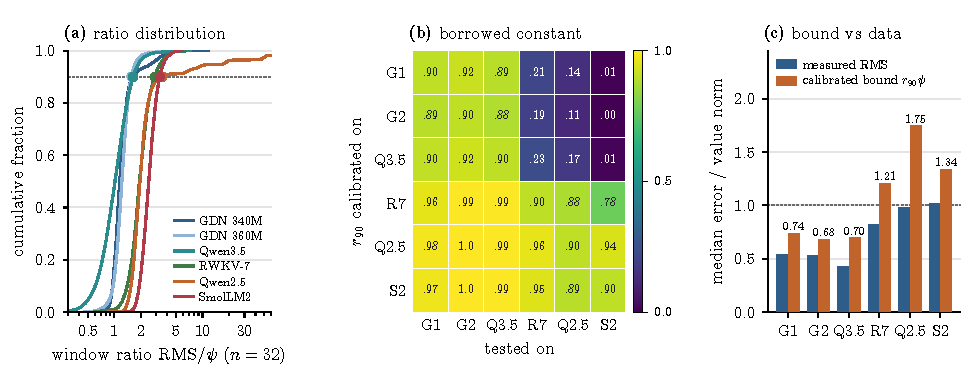
\includegraphics[width=\linewidth]{fig_cert.pdf}
  \caption{The calibrated key-only bound across six models ($n=32$). (a) Empirical distribution of the window ratio $\mathrm{RMS}/\psi$; the dots mark the 90th percentile, the pooled constant $r_{90}$. (b) Coverage of $\mathrm{RMS}\le r_{90}\psi$ when the constant is calibrated on the row model and tested on the column model: it is close to the nominal 0.90 within the delta-rule models and fails from the delta-rule models to RWKV-7 and the Transformers (G: Gated DeltaNet, Q: Qwen, R7: RWKV-7, S2: SmolLM2). (c) Median measured error and median calibrated bound; a bound above 1 is no better than storing nothing.}\label{fig:cert}
\end{figure}

\begin{figure}[t]
  \centering
  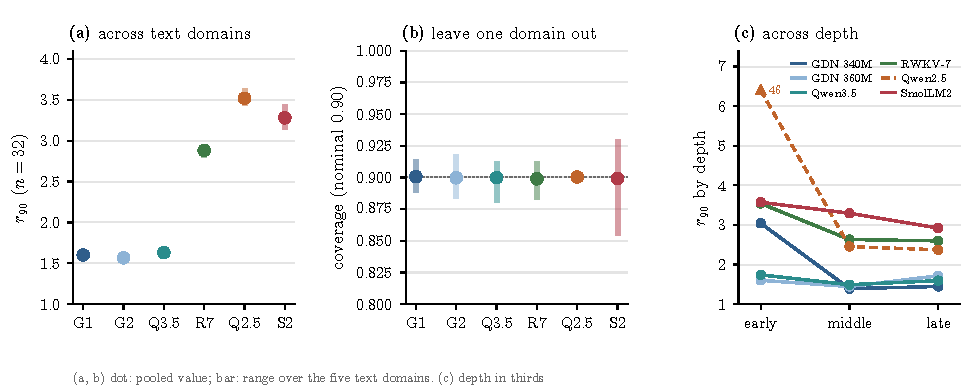
\includegraphics[width=\linewidth]{fig_cert2.pdf}
  \caption{Robustness of the calibrated constant ($n=32$). (a) $r_{90}$ in each of the five text domains (bar: range over the domains; dot: pooled constant). (b) Leave-one-domain-out coverage (dot: mean; bar: range over the five held-out domains; nominal 0.90). (c) $r_{90}$ by relative depth: in Qwen2.5 the first third of the layers has a constant of about 46 (off scale), driven by the first layers, whereas the other models vary by less than a factor of 2.}\label{fig:cert2}
\end{figure}

\begin{itemize}
  \item \textbf{Across text domains}: $r_{90}$ varies by $\pm0.03$--$0.05$ over the five domains and leave-one-domain-out coverage is 0.88--0.92 in all six models.
  \item \textbf{Across the three Gated-DeltaNet models} (two trainers, two corpora, different scale, a hybrid): mutual coverage of the pooled $r_{90}$ is 0.84--0.96 against a nominal 0.90.
  \item \textbf{To RWKV-7 and to Transformers}: no. The Gated-DeltaNet $r_{90}$ covers only 0.19--0.31 of RWKV-7 windows and 0.00--0.14 of Transformer windows; the Transformer $r_{90}$ covers 0.98--1.00 of the Gated-DeltaNet windows but with vacuous bounds ($\approx1.4$). RWKV-7's $r_{90}$ covers 0.96--0.99 of the delta-rule models' windows (conservative).
  \item \textbf{Across depth and head class within a model}: depth dependence replicates between the two Gated DeltaNets; class dependence does not; calibrating per head gives tighter bounds (0.49--0.57 for long heads) but slightly under-covers (mean coverage 0.87--0.89, worst decile 0.64--0.75).
\end{itemize}
\textbf{Held-out check on new text (post hoc).} Because the constants rest on 10--20 sequences per model, we applied the published $r_{90}$, unchanged, to sequences that were not used to calibrate them (protocol fixed beforehand: \texttt{exp\_heldout/PROTOCOL.md}): prose and code from APPS problems 600--1199 (the calibration sequences used problems 0--599), and docs and legal sequences taken at start positions interleaved between the calibration positions; the project-notes collection is not used. Each pipeline ran on its original number of sequences per domain (four for the Gated DeltaNets, three for the Transformers, two for RWKV-7 and Qwen3.5), \heldSeqLo--\heldSeqHi\ sequences per model in all. Table~\ref{tab:heldout} gives the coverage, the fraction of held-out windows with $\mathrm{RMS}\le r_{90}\psi_{\rm rms}$ (nominal 0.90), with 95\% cluster bootstraps over the new sequences. Coverage is \heldCovLo--\heldCovHi\ for all six models and both window sizes, and the criterion fixed in advance (an interval containing 0.90 or lying within 0.85--0.95, at both window sizes) is met by every model. The weakest is SmolLM2 (coverage 0.874 and 0.869, the widest intervals, from twelve sequences), whose held-out $r_{90}$ is about 5\% above the published value. The intervals of the Gated DeltaNets are narrow because all windows, heads and layers of a sequence are resampled together and the sequences vary little. The check supports stability of the constants on similar local text from the same sources; it is not a test of other domains.

\begin{table}[!htbp]
  \caption{Coverage of the published $r_{90}$ on held-out sequences (post hoc; 95\% cluster-bootstrap intervals over the new sequences). $n$: window size; held-out $r_{90}$: the 90th percentile of RMS/$\psi_{\rm rms}$ on the new sequences.}\label{tab:heldout}
  \centering\scriptsize\setlength{\tabcolsep}{4pt}
  \begin{tabular}{llcccc}
\toprule
model & $n$ & published $r_{90}$ & held-out $r_{90}$ & coverage (95\% CI) & sequences \\
\midrule
GDN 340M & 16 & 1.53 & 1.50 & .904 (.900, .907) & 16 \\
 & 32 & 1.60 & 1.58 & .904 (.901, .907) & 16 \\
\midrule
GDN 360M & 16 & 1.49 & 1.48 & .903 (.895, .911) & 16 \\
 & 32 & 1.57 & 1.55 & .906 (.899, .913) & 16 \\
\midrule
Qwen3.5-0.8B & 16 & 1.47 & 1.45 & .907 (.896, .917) & 8 \\
 & 32 & 1.63 & 1.61 & .908 (.899, .918) & 8 \\
\midrule
RWKV-7 0.1B & 16 & 2.67 & 2.55 & .916 (.910, .923) & 8 \\
 & 32 & 2.88 & 2.76 & .918 (.912, .925) & 8 \\
\midrule
Qwen2.5-1.5B & 16 & 3.44 & 3.53 & .898 (.892, .902) & 12 \\
 & 32 & 3.52 & 3.70 & .895 (.882, .903) & 12 \\
\midrule
SmolLM2-135M & 16 & 3.14 & 3.28 & .874 (.815, .910) & 12 \\
 & 32 & 3.28 & 3.43 & .869 (.803, .908) & 12 \\
\bottomrule
\end{tabular}

\end{table}

\textbf{Summary.} (i) The exact laws hold on every real recurrence tested. (ii) The keys' effective rank is small, which limits how many value directions a given norm budget can store (Theorem~\ref{thm:cap}); we give no single capacity number. (iii) The key--value structure that lowers interference is mostly a shared residual-stream latent, not a learnable key$\to$value map, so no comparator fitted outside the window certifies more than $n\approx8$. (iv) A calibrated value-free bound is informative and stable across the five text collections used; its level is set by how the value branch's rank compares with the key branch's, so it must be calibrated per model family, and the evidence for stability is two to four sequences per collection, plus a post hoc check on new sequences in which the published constants cover \heldCovLo--\heldCovHi\ of the windows. (v) None of this is a guarantee, and Section~\ref{sec:task} finds no detectable incremental association with task-level recall once distance is controlled. (vi) A key-only quantity that uses the model's own gates tracks the interference measured in the actual recurrence (Appendix~\ref{app:gate}, post hoc), which the gate-free quantity does not beyond short delays; it too adds no detectable information about recall (Appendix~\ref{app:gatetask}).

\subsection{A gate-aware key-only quantity in the actual recurrence (post hoc)}\label{app:gate}
\textbf{Why.} The key-only quantity $\psi$ of the main text is computed for an idealised memory ($\alpha=\beta=1$). The trained models write with their own gates; this subsection tests whether a key-only quantity that uses the real decay and write-strength gates, but still no values, tracks the interference measured in the actual recurrence, and whether it does so beyond decay and distance. The protocol was fixed before the runs (\texttt{exp\_gate/PROTOCOL.md}); the analysis is post hoc relative to the pre-registered test of Section~\ref{sec:task}, and its two additions (sixteen instead of eight sequences per model, a key-permutation control) are logged there.

\textbf{Quantities.} For a stored position $s$ and a delay $\Delta$ let $A=\prod_{u\in(s,s+\Delta]}\alpha_u$ be the designed retention. The measured interference is $D_{\rm act}=\|S_{s+\Delta}k_s-A\,S_sk_s\|/\|S_sk_s\|$ in the actual recurrence (the quantity of Figure~\ref{fig:decay}). The gate-aware key-only quantity $D_{\rm gate}$ is the same expression in the recurrence run with the model's real gates and its values replaced by its keys ($v_u=k_u$), so it is computed from keys and gates alone; Lemma~\ref{lem:interf} holds for it to a relative residual of $10^{-6}$. The comparators are $D_{\rm free}$, the gate-free idealised memory ($\alpha=\beta=1$, values equal to keys, started 32 tokens before $s$); $D_{\rm shuf}$, which is $D_{\rm gate}$ with the keys permuted over positions and the real gates kept (a key-specificity control); and $B_{\rm key}=\sum_{u}\beta_u|\langle k_u,k_s\rangle|$, the gate-weighted key overlap without a recurrence.

\textbf{Design.} Both Gated DeltaNets, every layer and head, sixteen 1024-token sequences each (eight prose, eight code), probes $s\in\{64,128,\dots,512\}$ and delays $\Delta\in\{16,64,256,512\}$ (cells with $s+\Delta>1023$ are dropped). Spearman correlations are taken within each (layer, head, delay) group, so they ask which positions suffer more interference in a given head, and are then averaged over groups; ``decay removed'' is the partial correlation after removing the rank of $\log A$; intervals are 95\% cluster bootstraps over the sixteen sequences (500 resamples). Long-memory heads are those whose median decay half-life exceeds 256 tokens in these sequences (28 of 96 heads in the 340M model, 27 of 84 in the 360M model).

\begin{figure}[!htbp]
  \centering
  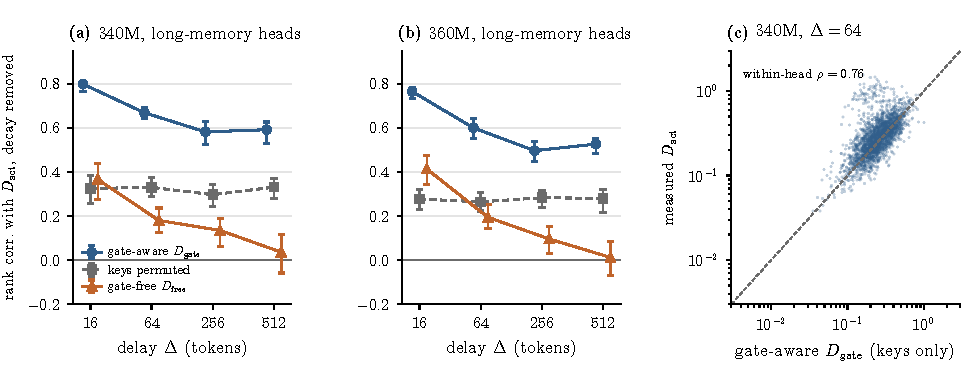
\includegraphics{fig_gate.pdf}
  \caption{A gate-aware key-only quantity against the interference measured in the actual recurrence (post hoc). (a, b) Rank correlation, within head and with the decay gate removed, of the measured interference $D_{\rm act}$ with the gate-aware key-only quantity $D_{\rm gate}$, with the same quantity computed with permuted keys, and with the gate-free idealised-memory quantity, by delay, in long-memory heads (95\% cluster bootstrap over sixteen sequences). (c) The cells behind (a) at $\Delta=64$ in the 340M model (long-memory heads, all probes and sequences; 2500 drawn at random).}\label{fig:gate}
\end{figure}

\begin{table}[!htbp]
  \caption{Rank correlation of the measured interference $D_{\rm act}$ with key-only predictors in long-memory heads: within head ($D_{\rm gate}$) and after removing the decay gate (partial; 95\% cluster-bootstrap intervals). $D_{\rm shuf}$: keys permuted; $D_{\rm free}$: gate-free idealised memory; $B_{\rm key}$: gate-weighted key overlap.}\label{tab:gateactual}
  \centering\scriptsize\setlength{\tabcolsep}{3pt}
  \begin{tabular}{llccccc}
\toprule
model & delay & $D_{\rm gate}$, within & $D_{\rm gate}$, decay removed & $D_{\rm shuf}$ & $D_{\rm free}$ & $B_{\rm key}$ \\
\midrule
GDN 340M & 16 & .86 & .80 (.77, .81) & .32 (.26, .38) & .37 (.27, .44) & .65 (.61, .68) \\
 & 64 & .76 & .67 (.64, .69) & .33 (.29, .37) & .18 (.13, .24) & .41 (.36, .46) \\
 & 256 & .70 & .58 (.52, .63) & .30 (.24, .34) & .13 (.06, .19) & .10 (.02, .19) \\
 & 512 & .68 & .59 (.53, .63) & .33 (.28, .37) & .04 ($-$.06, .12) & .06 ($-$.01, .13) \\
\midrule
GDN 360M & 16 & .84 & .76 (.73, .78) & .28 (.23, .32) & .41 (.34, .47) & .66 (.63, .67) \\
 & 64 & .70 & .60 (.55, .64) & .26 (.22, .31) & .19 (.14, .25) & .44 (.39, .48) \\
 & 256 & .57 & .50 (.45, .54) & .28 (.24, .32) & .10 (.03, .15) & .12 (.06, .18) \\
 & 512 & .57 & .53 (.48, .55) & .28 (.22, .32) & .01 ($-$.07, .09) & .01 ($-$.03, .07) \\
\bottomrule
\end{tabular}

\end{table}

\textbf{Result.} (Figure~\ref{fig:gate}, Table~\ref{tab:gateactual}.) In long-memory heads $D_{\rm gate}$ tracks the measured interference with a partial within-head rank correlation of \gatePartLo--\gatePartHi\ over delays of 16 to 512 tokens in both models (all heads: \gateAllPartLo--\gateAllPartHi). The gate-free $D_{\rm free}$ gives \freePartLo--\freePartHi\ and falls to about zero at 512 tokens, and $D_{\rm shuf}$, with the real gates but permuted keys, gives \shufPartLo--\shufPartHi. The criterion fixed in advance (a partial correlation of at least 0.3 with an interval excluding 0, exceeding the gate-free quantity by more than the interval width) is met at every delay in both models.

\textbf{Reading and limits.} The gate-aware key-only quantity is a usable measurement of the interference that actually occurs, which the gate-free quantity is not beyond short delays. That the permuted-keys control retains about 0.3 shows that part of the signal is carried by the gates' own profile along the sequence, and the key geometry accounts for the rest. $D_{\rm act}$ and $D_{\rm gate}$ share keys and gates by construction, so the correlation measures how much of the interference is set by keys and gates rather than by values. It is two small models of one family, two text domains and sequences of 1024 tokens; it is not a prediction of recall, which is the subject of Appendix~\ref{app:gatetask}.

%==============================================================================
\section{Training-time experiment: details}\label{app:lever}
\subsection{Design}
\textbf{Task.} A sequence contains $n$ (key, value) token pairs (keys drawn without replacement from 64 key tokens, values from 64 value tokens), then $L$ filler tokens, then the $n$ keys again in random order. Training: $n\in[4,32]$, $L\in[0,96]$. Evaluation: $n\in\{8,16,24,32\}$, $L\in\{0,32,96\}$, 128 sequences per cell. \textbf{Model.} Embedding $\to$ $2\times$[gated delta-rule layer (2 heads, $d_k=d_v=32$, depthwise causal convolution of width 4 with SiLU on $q,k,v$, $L_2$-normalised $q,k$, $\beta=\sigma(\cdot)$, $\alpha=\exp(-\exp(A_{\log})\,\mathrm{softplus}(\cdot))$, output gate) + SwiGLU MLP] $\to$ logits; 113{,}032 parameters; AdamW, one-cycle schedule, batch 64, 3000 steps. The delta-rule layer is the chunked reference implementation (equal to a step-by-step loop to $7\times10^{-8}$ forward and $3\times10^{-7}$ in gradients); the depthwise convolution is a shift-and-sum implementation (equal to the library convolution to $10^{-6}$).

\textbf{Regularisers} (task-agnostic; computed from the layer's own keys and values on the first 16 positions of every sequence): key decorrelation (weight 1), Gram matching (weight 1; $\mathrm{mean}(H-G)^2_{\mathrm{offdiag}}$), rank matching (weight 0.1; $\max(0,r_{\mathrm{eff}}(V)-r_{\mathrm{eff}}(K))$). Chosen from the theory before any run; each has one untuned weight.

\subsection{Per-seed results}
\begin{table}[!htbp]
  \caption{Mean recall accuracy per seed (over $n=8..32$, $L=0/32/96$) and the first logged step at which cross-entropy fell below 2 (``--'': never).}
  \centering\scriptsize\setlength{\tabcolsep}{2.5pt}
  \begin{tabular}{lcccccccccccc}
\toprule
seed & 0 & 1 & 2 & 3 & 4 & 5 & 6 & 7 & 8 & 9 & 10 & 11 \\
\midrule
baseline & .58 & .95 & .96 & .96 & .86 & .98 & .36 & .95 & .98 & .11 & .99 & .97 \\
\quad escape step & 1500 & 1000 & 1250 & 1000 & 1750 & 1000 & 2000 & 1000 & 1250 & 1250 & 750 & 750 \\
key decorrelation & .95 & .99 & .93 & .98 & .97 & .98 & .96 & .94 & .99 & .98 & .98 & .98 \\
\quad escape step & 1000 & 750 & 1000 & 1000 & 1000 & 1000 & 1000 & 1000 & 750 & 1000 & 1000 & 750 \\
Gram matching & .96 & .02 & .56 & .82 & .25 & 1.00 & .89 & .95 & .98 & .97 & .78 & .97 \\
rank matching & .27 & .66 & .94 & .55 & .59 & .98 & .81 & .97 & .11 & .89 & .98 & .98 \\
\bottomrule
\end{tabular}

\end{table}

\subsection{Geometry of the trained models}
Median over sequences and heads, first 16 positions of an $n=16$, $L=32$ evaluation batch:
\begin{table}[!htbp]
  \caption{Median key and value effective ranks, their ratio, the mean gain $q$ and $\mathrm{RMS}/\psi$ of the first 16 positions (layer 0 / layer 1; pooled over all runs of a learner, sequences and heads).}\label{tab:geom}
  \centering\small\setlength{\tabcolsep}{4pt}
  \begin{tabular}{lccccc}
\toprule
learner & key $r_{\mathrm{eff}}$ & value $r_{\mathrm{eff}}$ & values/keys & $q$ & $\mathrm{RMS}/\psi$ \\
\midrule
baseline & 8.80 / 2.00 & 6.84 / 4.95 & 0.79 / 1.59 & 2.43 / 14.88 & 1.58 / 2.16 \\
key decorrelation & 11.43 / 11.52 & 7.25 / 4.67 & 0.63 / 0.43 & 1.59 / 1.39 & 1.39 / 1.26 \\
Gram matching & 3.11 / 1.12 & 3.11 / 1.13 & 1.00 / 1.00 & 1.13 / 4.20 & 1.00 / 1.07 \\
rank matching & 9.97 / 3.27 & 6.69 / 1.59 & 0.68 / 0.75 & 1.88 / 2.71 & 1.45 / 1.17 \\
\bottomrule
\end{tabular}

\end{table}

\begin{figure}[!htbp]
  \centering
  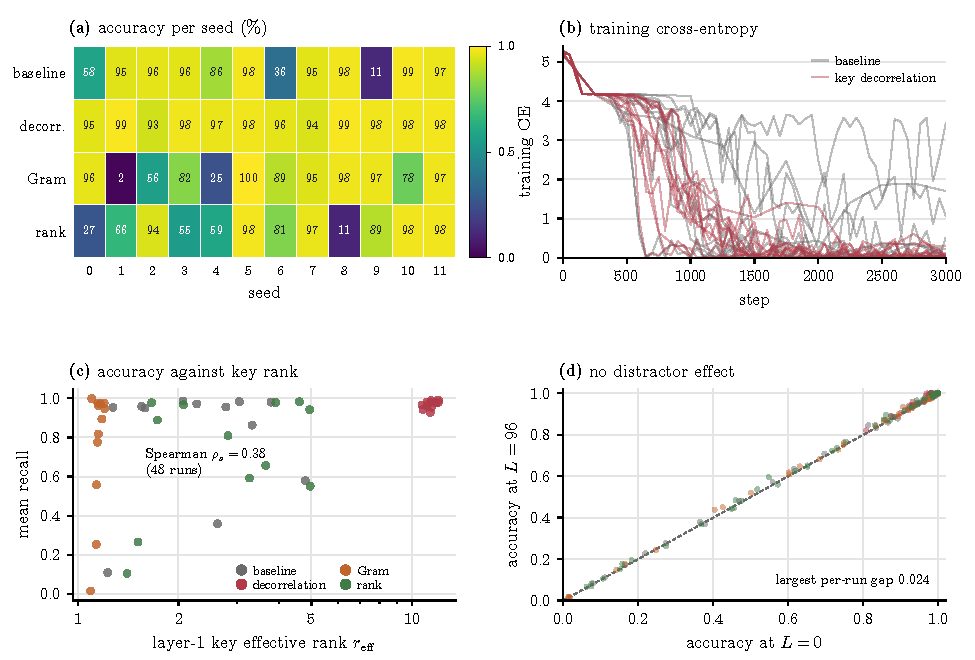
\includegraphics[width=\linewidth]{fig_lever_app.pdf}
  \caption{Details of the training-time experiment. (a) Mean recall of every run of seeds 0--11 (percent). (b) Training cross-entropy of every baseline and key-decorrelation run. (c) Accuracy against the layer-1 key effective rank over all \mqNRuns\ runs (Spearman correlation in the panel). (d) Accuracy at $L=96$ against $L=0$ for every run and $n$: the points lie on the diagonal, so the task is insensitive to the tested distractor lengths. The effective ranks and gains of every learner are in Table~\ref{tab:geom}.}\label{fig:leverapp}
\end{figure}
Across all \mqNRuns\ runs the accuracy rank-correlates with the keys' effective rank (layer 1: Spearman $\mqSpKey$; the smaller of the two layers' ranks: $\mqSpMin$) and more weakly with the values' ($\mqSpValZero,\mqSpVal$).

\subsection{Interpretation and caveats}
In the first twelve seeds the baseline's second layer collapses to a key rank of 2.0 with values of rank 5.0, the regime of RWKV-7 and the Transformers in Section~\ref{sec:measure}; decorrelation holds the key rank at 11.5 (ratio 0.43, $q=1.39$), the regime the trained Gated DeltaNets naturally occupy, and across the \mqNRuns\ runs of seeds 0--11 the accuracy rank-correlates with the key rank. The new seeds (Appendix~\ref{app:leverrep}) show that the regulariser does raise the key rank but that the rank does not predict success there, so the geometric account is not supported as a cause of failures to learn. \emph{Flat gain is a symptom, not a target}: Gram matching drives $\mathrm{RMS}/\psi$ to \gramRmsLo--\gramRmsHi\ without helping, by shrinking both ranks to \gramRankLo--\gramRankHi, the capacity-floor regime. In the first twelve seeds the benefit of decorrelation was \emph{preventing failures to learn} (a long plateau at chance), not a general capacity increase: when the baseline learned, recall was within $\mqGainRest$ of the decorrelated model's on average. That did not replicate.

\textbf{Caveats.} One task and one small model; one untuned weight per regulariser (a weight of 1 for decorrelation was used throughout; larger or smaller weights, and decorrelation on the \emph{value} branch, were not tried); three regularisers were compared, so the first $p\approx0.04$ is $\mqHolm$ after a Holm correction; seeds 0--5 were run with coarser logging than seeds 6--11 (the escape-step analysis uses the common 250-step grid). The evidence that decorrelation helps did not replicate, and with twelve seeds each the matching and rank regularisers show no detectable effect.

\subsection{Replication with new seeds (post hoc extension)}\label{app:leverrep}
\textbf{Why and how.} The first experiment (seeds 0--11) was a single comparison with an uncorrected $p=\mqSF$, and the matching regularisers had fewer seeds. Under a protocol fixed beforehand (\texttt{exp\_mqar/\allowbreak PROTOCOL\_replication.md}) we ran twelve new seeds (12--23) of the baseline and of key decorrelation with the identical configuration (the runs differ from the first ones only in the seed), and completed the Gram-matching and rank-matching runs to twelve seeds each. The effect counts as replicated if the paired difference is positive, its interval excludes zero and the exact two-sided sign-flip $p<0.05$.

\begin{figure}[!htbp]
  \centering
  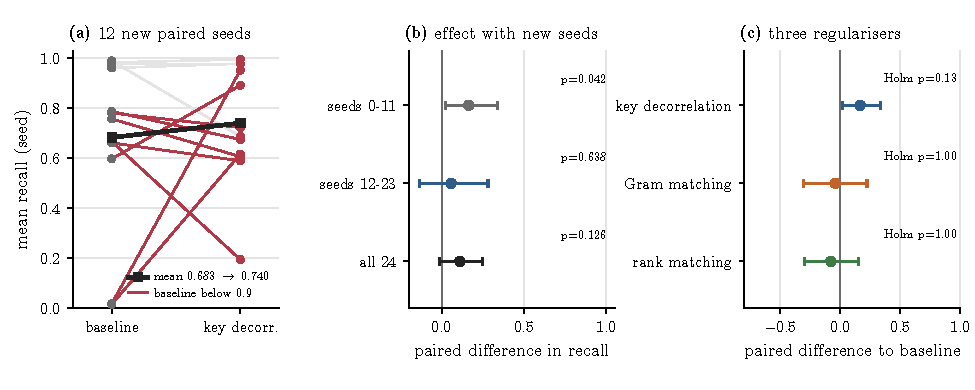
\includegraphics{fig_lever_rep.pdf}
  \caption{Replication of the key-decorrelation effect (post hoc extension). (a) Paired seeds 12--23: baseline against key decorrelation (red lines: baseline below 0.9 mean recall; black: mean). (b) Paired difference (95\% bootstrap interval) in the first twelve seeds, the new twelve and all 24, with the exact sign-flip $p$. (c) The three regularisers against the baseline over seeds 0--11 (twelve seeds each; Holm-adjusted $p$ over the three).}\label{fig:leverrep}
\end{figure}

\begin{table}[!htbp]
  \caption{The key-decorrelation comparison by seed set. Paired difference with its 95\% bootstrap interval, number of seeds in which decorrelation is higher, exact sign-flip and Wilcoxon $p$, and the number of runs below 0.9 mean recall (baseline/decorrelation).}\label{tab:leverrep}
  \centering\scriptsize\setlength{\tabcolsep}{3pt}
  \begin{tabular}{lccccccc}
\toprule
seeds & baseline & decorr. & paired difference & higher & sign-flip $p$ & Wilcoxon $p$ & below 0.9 \\
\midrule
0--11 & .804 & .969 & $+$.165 ($+$.021, $+$.337) & 8/12 & .042 & .064 & 4/0 \\
12--23 & .683 & .740 & $+$.058 ($-$.136, $+$.282) & 5/12 & .638 & .850 & 8/8 \\
all 24 & .743 & .854 & $+$.111 ($-$.015, $+$.251) & 13/24 & .126 & .345 & 12/8 \\
\bottomrule
\end{tabular}

\end{table}

\textbf{Result.} The criterion is not met: in the new seeds the paired difference is $\repDiff$ ($[\repCiLo,\repCiHi]$), \repHigher\ of 12 seeds higher, sign-flip $p=\repSF$ (Table~\ref{tab:leverrep}, Figure~\ref{fig:leverrep}). Both learners have a wide spread of seeds in the new runs, from near zero to above 0.98 mean recall, and \repFailBase\ of 12 baseline and \repFailDec\ of 12 decorrelated runs stay below 0.9, against \mqFailBase\ and \mqFailDec\ in the first twelve seeds; pooled over 24 seeds the difference is $\poolDiff$ ($[\poolCiLo,\poolCiHi]$, $p=\poolSF$). As exploratory checks, in the 24 new runs key decorrelation raises the layer-1 key effective rank (median \mqNewKeyDec\ against \mqNewKeyBase\ for the baseline) as designed, but the accuracy no longer tracks it (Spearman $\mqNewSp$; median rank \mqNewFailRank\ in runs below 0.9 against \mqNewLearnRank\ in the others). With twelve seeds each, Gram matching and rank matching differ from the baseline by $\matchDiff$ ($p=\matchSF$, Holm-adjusted $\matchHolm$) and $\rankDiff$ ($p=\rankSF$, $\rankHolm$), and key decorrelation by $\mqDiff$ ($p=\mqSF$, Holm-adjusted $\mqHolm$) in seeds 0--11. We conclude that the training-time experiment gives no reliable evidence that key decorrelation improves training in this model: the first twelve seeds were a favourable draw of a high-variance process, or the effect is smaller and needs more seeds than we ran.

%==============================================================================
\section{Task-level test: details}\label{app:task}
\subsection{Pre-registration summary}
The pre-registration (written before any prompt was run through the models) fixed: the two models; the task; the predictors; the 50/50 calibration/test split by prompt; the primary hypothesis H1 and its criterion; the secondary analyses (shuffled-$\psi$ control, a decision-style tercile comparison); and the statement that failure to meet H1 in either model would be reported as such with no change to predictors, thresholds, head definition or analysis after seeing test outcomes. Two changes were made and logged:
\begin{itemize}
  \item \textbf{Amendment A} (after an accuracy-only pilot, before any bound was computed). Strict top-1 over the vocabulary was 0.05--0.15 at every load while forced-choice recall was 0.60/0.40/0.30/0.20/0.07 at $n=2/4/8/16/32$ against chance 0.50/0.25/0.125/0.06/0.03; the primary outcome became forced-choice correct, the load levels $\{4,8,16,24\}$, and $n$ was included as a baseline.
  \item \textbf{Deviation D1} (an implementation error, not outcome-driven). The extraction stored each head's mean log-decay per prompt, while the protocol defines long-memory heads by the \emph{median per-token half-life}; the first analysis therefore found 0 long-memory heads and $P_1$ was undefined. The head groups were recomputed from calibration prompts only (10 per load) and no outcome information entered the definition. The first run's secondary numbers were seen.
\end{itemize}
The pre-registered baseline modelled age linearly together with the one-hot load; this turned out to under-control age, which the exploratory analysis below exposes.

\subsection{Pilot (accuracy only, 40 prompts per load, Gated DeltaNet 340M)}
\begin{table}[!htbp]
  \centering\scriptsize\setlength{\tabcolsep}{3.5pt}
  \begin{tabular}{lccccc}
    \toprule
    facts $n$ & 2 & 4 & 8 & 16 & 32 \\
    \midrule
    strict top-1 over the vocabulary & .12 & .10 & .07 & .15 & .05 \\
    forced-choice recall & .60 & .40 & .30 & .20 & .07 \\
    chance & .50 & .25 & .125 & .06 & .03 \\
    \bottomrule
  \end{tabular}
\end{table}

\subsection{Full results}
\begin{table}[!htbp]
  \caption{Test-set AUC for forced-choice recall (pooled over loads; 300 test prompts per model). $P_1$ and $P_{1b}$ enter with the sign that predicts recall.}\label{tab:taskfull}
  \centering\small\setlength{\tabcolsep}{4pt}
  \begin{tabular}{lcc}
\toprule
predictor & GDN 340M & GDN 360M \\
\midrule
age & .676 & .603 \\
load $n$ & .625 & .524 \\
age + one-hot load (B3) & .644 & .575 \\
$P_1$ (long-memory heads) & .615 & .626 \\
$P_{1b}$ (all heads) & .602 & .621 \\
$P_1$ shuffled within load & .534 & .551 \\
B3 + $P_1$ & .644 & .693 \\
B3 + $P_{1b}$ & .638 & .664 \\
B3 + shuffled $P_1$ & .645 & .538 \\
\midrule
H1: AUC(B3+$P_1$) $-$ AUC(B3), 95\% CI & $\pm$.000 ($-$.041, $+$.038) & $+$.118 ($+$.056, $+$.182) \\
AUC(B3+$P_1$) $-$ AUC(B3+shuffled), 95\% CI & $-$.001 ($-$.039, $+$.038) & $+$.155 ($+$.084, $+$.225) \\
\bottomrule
\end{tabular}

\end{table}
\textbf{Within each load} (test prompts, AUC of $P_1$ alone / shuffled / age): 340M: $n{=}4$ .361/.462/.372; $n{=}8$ .333/.466/.319; $n{=}16$ .433/.355/.404; $n{=}24$ .455/.540/.436. 360M: $n{=}4$ .268/.433/.288; $n{=}8$ .219/.414/.255; $n{=}16$ .490/.467/.473; $n{=}24$ .558/.470/.558. Within a load $P_1$ tracks age almost exactly. \textbf{Decision test} (lowest minus highest $P_1$ tercile within a load, weighted): $+0.14$ (340M), $+0.23$ (360M), confounded in the same way.

\subsection{Exploratory analysis: why the pooled gain disappears}
\begin{figure}[!htbp]
  \centering
  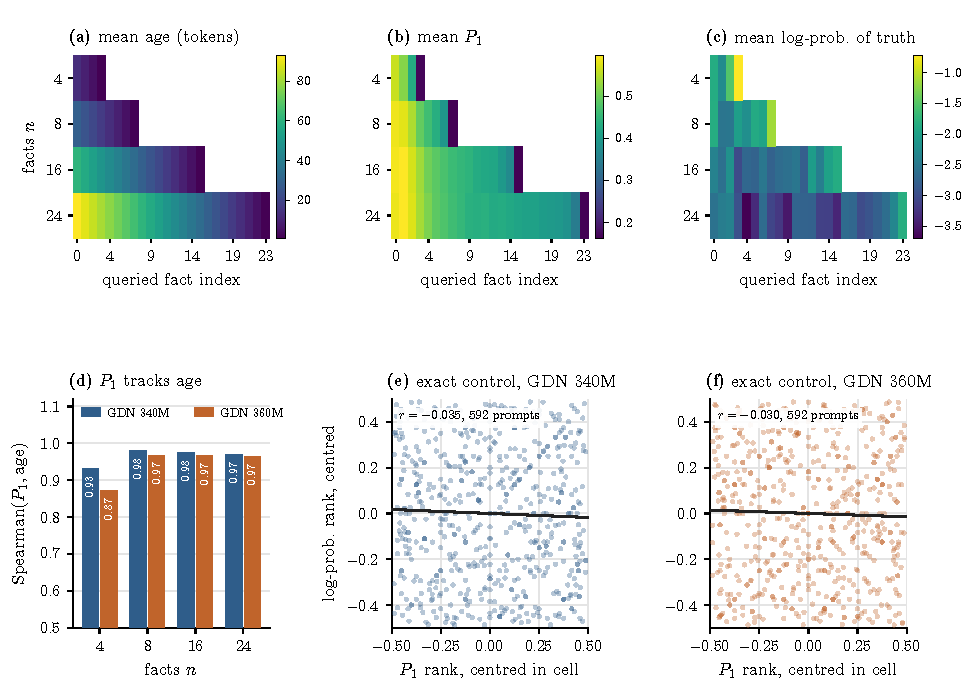
\includegraphics[width=\linewidth]{fig_task_app.pdf}
  \caption{Why the pooled gain disappears (top: Gated DeltaNet 340M; each cell holds the prompts with one load and one queried position, hence one age). (a, b) The mean age and the mean $P_1$ of a cell have the same structure across loads and positions. (c) The mean log-probability of the true value. (d) Within a load, $P_1$ is nearly collinear with age. (e, f) With age fixed exactly, the ranks of $P_1$ and of the log-probability, centred within their cell, are uncorrelated.}\label{fig:taskapp}
\end{figure}

\begin{figure}[!htbp]
  \centering
  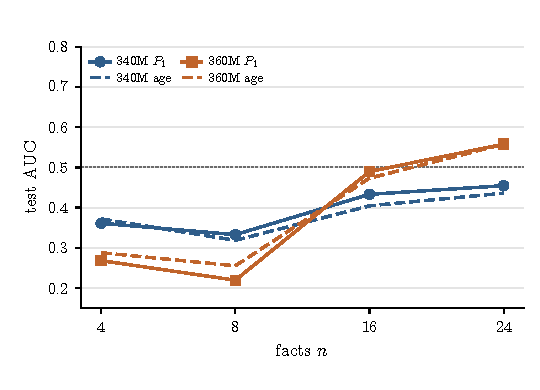
\includegraphics{fig_task_roc.pdf}
  \caption{Test AUC of $P_1$ and of age alone within each load, for the two Gated DeltaNets (below 0.5: higher values predict worse recall).}\label{fig:taskroc}
\end{figure}
\begin{table}[!htbp]
  \caption{Partial rank correlation of $P_1$ with the true value's candidate log-probability (negative: higher $\psi$ $\Rightarrow$ worse recall).}
  \centering\scriptsize\setlength{\tabcolsep}{3.5pt}
  \begin{tabular}{lcc>{\raggedright\arraybackslash}p{3.0cm}}
    \toprule
    control & GDN 340M & GDN 360M & note \\
    \midrule
    age linear + one-hot load (test) & $-0.228$ ($-.339,-.115$) & $-0.400$ ($-.497,-.299$) & as pre-registered \\
    shuffled within load (null) & $-0.062$ ($-.163,+.045$) & $-0.078$ ($-.189,+.035$) & \\
    $P_{1b}$ (all heads) & $-0.236$ & $-0.368$ & \\
    short-memory heads & $-0.244$ & $-0.352$ & not specific to long heads \\
    whole-prefix mean $\psi$ & $+0.037$ & $+0.099$ & no signal \\
    per load, age linear: $n{=}4/8/16/24$ & $-.08/-.08/-.05/-.15$ & $-.24/-.41/-.09/+.03$ & weaker within a load \\
    \textbf{exact: within (load, query position) cells} & $\mathbf{-0.035}$ $(-.121,+.041)$ & $\mathbf{-0.030}$ $(-.108,+.049)$ & identical age \\
    exact control, shuffled null & $0.000$ ($-.075,+.081$) & $-0.005$ ($-.085,+.070$) & \\
    exact control, $P_{1b}$ / short heads & $-.088$ / $-.080$ & $-.007$ / $-.006$ & \\
    exact control, outcome = forced-choice correct & $+0.036$ & $+0.018$ & \\
    \bottomrule
  \end{tabular}
\end{table}
Age is a deterministic function of the queried position for a given load, so cells of (load, queried position) hold age fixed exactly (48 cells, 592 prompts with at least 4 per cell). Within those cells no detectable association remains in either model. The pooled correlations are explained by age entering the pre-registered baseline only linearly: $P_1$ proxies a nonlinear age effect. \textbf{By layer block} (long-memory heads, controls age + load) the pooled partial correlations are the same in every block ($-0.26$ to $-0.27$ in the 340M model; $-0.32$ to $-0.41$ in the 360M model), i.e.\ not localised to any depth.

\subsection{Held-out AUC with a flexible categorical age adjustment (post hoc)}
The pre-registered baseline (age linear plus one-hot load) under-controls age, and the exact within-cell analysis is a stratified rank correlation, not an AUC. To compare held-out discrimination under a flexible categorical age adjustment we fit a logistic model on the calibration prompts whose features are a fixed effect for every (load, queried position) cell (and for the load), with and without $P_1$, and compare AUC on the test prompts (paired bootstrap over test prompts, 2000 resamples). This analysis was added after the others; the ridge weight $\lambda=1$ was fixed before inspection and the results are shown for $\lambda\in\{0.3,1,3\}$.
\begin{table}[!htbp]
  \caption{Held-out AUC with a flexible categorical age adjustment (cell fixed effects), without and with $P_1$.}\label{tab:flexauc}
  \centering\small\setlength{\tabcolsep}{4pt}
  \begin{tabular}{lcccc}
\toprule
model & ridge $\lambda$ & AUC cell effects & AUC $+P_1$ & $\Delta$ (95\% CI) \\
\midrule
GDN 340M & 0.3 & .661 & .663 & $+$.002 ($-$.017, $+$.019) \\
GDN 340M & 1 & .661 & .662 & $+$.001 ($-$.017, $+$.017) \\
GDN 340M & 3 & .662 & .661 & $-$.002 ($-$.019, $+$.014) \\
GDN 360M & 0.3 & .649 & .648 & $-$.001 ($-$.008, $+$.007) \\
GDN 360M & 1 & .647 & .648 & $\pm$.000 ($-$.006, $+$.007) \\
GDN 360M & 3 & .646 & .648 & $+$.002 ($-$.005, $+$.009) \\
\bottomrule
\end{tabular}

\end{table}
Adding $P_1$ changes held-out AUC by at most $0.002$ in absolute value and the intervals are within $\pm0.02$ (340M) and $\pm0.01$ (360M), so the upper endpoint of the interval is below $0.02$ (340M) and $0.01$ (360M) for this fitted comparison. The bootstrap resamples test prompts with the fitted models held fixed: it quantifies the performance difference of these two fitted predictors given the calibration data, and does not exclude nonlinear predictors, interactions, other fitting procedures, or variation due to the training sample.

\subsection{Why this null may be regime-specific}
Prompts have at most about 100 tokens against a state of $d_k=256$, so the state need not saturate; $\psi$ uses $\alpha=\beta=1$ while the heads carrying long-range recall have decay gates; forced-choice accuracy is low (0.17--0.46). A gate-aware key-only predictor, which tracks the interference in the actual recurrence (Appendix~\ref{app:gate}), was tested next (Appendix~\ref{app:gatetask}) and does not change the null. A larger model (1.3B) was tested too (Appendix~\ref{app:scale}) and does not change the picture, but its recall in this format is as weak as that of the small models. Prompts of 500--1000 tokens (64--96 facts) and a model with stronger recall would test whether the null is a property of the bound or of the regime. We did not run them.

\subsection{A gate-aware predictor at the task level (post hoc)}\label{app:gatetask}
Appendix~\ref{app:gate} defines a key-only quantity, $D_{\rm gate}$, that uses the model's real gates and tracks the interference in the actual recurrence. We computed it for the queried fact of every prompt of Section~\ref{sec:task} (same prompts, calibration/test split and long-memory heads; protocol \texttt{exp\_gate/PROTOCOL.md}, fixed before the run): for each of the three span tokens $s$ (key, ``is'', value), $D_{\rm gate}$ from $s$ to the last prefix token, averaged over the span and over the long-memory heads ($P_{1g}$); the retention $\|S_Tk_s\|/\|S_sk_s\|$ in the same recurrence ($P_{1r}$); the decay gate alone ($-\log A$); $P_{1g}$ shuffled within load; and $P_{1g}$ over all heads. The criterion fixed in advance was a held-out AUC gain of at least 0.03 over the flexible categorical-age baseline with an interval excluding 0 in the primary model and the same sign in the replication.

\begin{table}[!htbp]
  \caption{Gate-aware key-only predictors of task-level recall (post hoc; 95\% bootstrap intervals). $\Delta$AUC: held-out gain from adding the predictor to age and one-hot load (as pre-registered) or to a fixed effect for every (load, queried position) cell; within-cell $\rho$: rank correlation with the true value's log-probability among the candidates, within exact (load, queried position) cells. Thirty intervals in all, uncorrected.}\label{tab:gatetask}
  \centering\scriptsize\setlength{\tabcolsep}{3pt}
  \begin{tabular}{llccc}
\toprule
model & predictor & $\Delta$AUC, age + load & $\Delta$AUC, flexible age & within-cell $\rho$ \\
\midrule
GDN 340M & $P_{1g}$, gate-aware (long-memory heads) & $+$.004 ($-$.030, $+$.036) & $+$.005 ($-$.015, $+$.023) & $-$.036 ($-$.118, $+$.048) \\
 & $P_{1r}$, retention & $+$.004 ($-$.028, $+$.034) & $+$.003 ($-$.020, $+$.024) & $+$.026 ($-$.053, $+$.101) \\
 & decay only, $-\log A$ & $+$.001 ($-$.011, $+$.013) & $+$.006 ($-$.010, $+$.020) & $-$.038 ($-$.115, $+$.048) \\
 & $P_{1g}$ shuffled within load & $-$.010 ($-$.021, $\pm$.000) & $-$.008 ($-$.024, $+$.007) & $-$.040 ($-$.127, $+$.043) \\
 & $P_{1g}$, all heads & $\pm$.000 ($-$.047, $+$.044) & $-$.001 ($-$.021, $+$.019) & $+$.105 ($+$.024, $+$.191) \\
\midrule
GDN 360M & $P_{1g}$, gate-aware (long-memory heads) & $+$.022 ($-$.014, $+$.059) & $+$.003 ($-$.003, $+$.009) & $-$.045 ($-$.128, $+$.039) \\
 & $P_{1r}$, retention & $+$.006 ($-$.016, $+$.029) & $+$.003 ($-$.004, $+$.010) & $-$.074 ($-$.149, $+$.004) \\
 & decay only, $-\log A$ & $+$.001 ($-$.012, $+$.012) & $+$.001 ($-$.008, $+$.009) & $-$.057 ($-$.137, $+$.026) \\
 & $P_{1g}$ shuffled within load & $-$.047 ($-$.077, $-$.015) & $+$.001 ($-$.007, $+$.008) & $-$.014 ($-$.104, $+$.070) \\
 & $P_{1g}$, all heads & $+$.085 ($+$.028, $+$.140) & $+$.011 ($+$.001, $+$.021) & $-$.091 ($-$.181, $-$.011) \\
\bottomrule
\end{tabular}

\end{table}

\textbf{Result.} $P_{1g}$ adds no detectable information about recall beyond the flexible age baseline: the gain is $\gFlexDa$ ($\gFlexLoa$, $\gFlexHia$) in the 340M model and $\gFlexDb$ ($\gFlexLob$, $\gFlexHib$) in the 360M model, and its exact within-cell correlation with the true value's log-probability is $\gWithinRa$ ($\gWithinLoa$, $\gWithinHia$) and $\gWithinRb$ ($\gWithinLob$, $\gWithinHib$); the criterion is not met. $P_{1g}$ remains collinear with age (rank correlation \gCorrAgeA\ and \gCorrAgeB), which is why the pre-registered baseline, which models age only linearly, leaves room for apparent gains. Apart from the shuffled control in the 360M model (whose gain over age and load is negative), four of the thirty intervals exclude zero, all for the all-heads predictor: the pre-registered-style gain ($+0.085$), the flexible-age gain ($+0.011$) and the within-cell correlation ($-0.091$, the expected direction) in the 360M model, and a within-cell correlation of the opposite sign ($+0.105$) in the 340M model. The pre-registered-style gain in the 360M model disappears under the flexible age baseline, as it does for $P_1$ in Section~\ref{sec:task}; none of the four reaches the criterion, the signs disagree between models, and with thirty uncorrected comparisons we do not read them as an effect. The decay-only control behaves like the gate-aware predictor. So the task-level null of Section~\ref{sec:task} is not an artefact of ignoring the gates; what remains untested is whether it holds for prompts of 500--1000 tokens or for models with stronger recall (a larger model, Appendix~\ref{app:scale}, recalls no better in this format).

\subsection{A larger model (post hoc extension)}\label{app:scale}
\textbf{Why and how.} The models of Section~\ref{sec:task} are small and recall weakly. We repeated the test on \texttt{linear-moe-hub/Gated-Deltanet-1.3B}, a Gated DeltaNet of the same hub and family with 1.21B parameters (24 layers, hidden size 2048, four heads of dimension 256, trained on SlimPajama), under a protocol fixed before any prompt was run (\texttt{exp\_scale/PROTOCOL.md}). The checkpoint has no short convolution; our re-implementation then uses SiLU of the projection, and it agrees with the HuggingFace gated-delta-rule layer (identity convolution kernel) to a relative layer error of at most $4.3\times10^{-6}$ and logits to $1.3\times10^{-3}$ at logit scale 16--17, with identical top-1 predictions and perplexity (Table~\ref{tab:validation}). Prompts, split, outcome, head definition and analyses are those of Section~\ref{sec:task} and Appendix~\ref{app:task}; an accuracy-only pilot (20 prompts per load) showed that recall is not at ceiling, so the protocol's rule for extending the loads was not triggered. The predictors are the gate-free $P_1$ and $P_{1b}$ and the gate-aware ones of Appendix~\ref{app:gatetask}; \scLong\ of the \scHeads\ heads are long-memory heads.

\begin{figure}[!htbp]
  \centering
  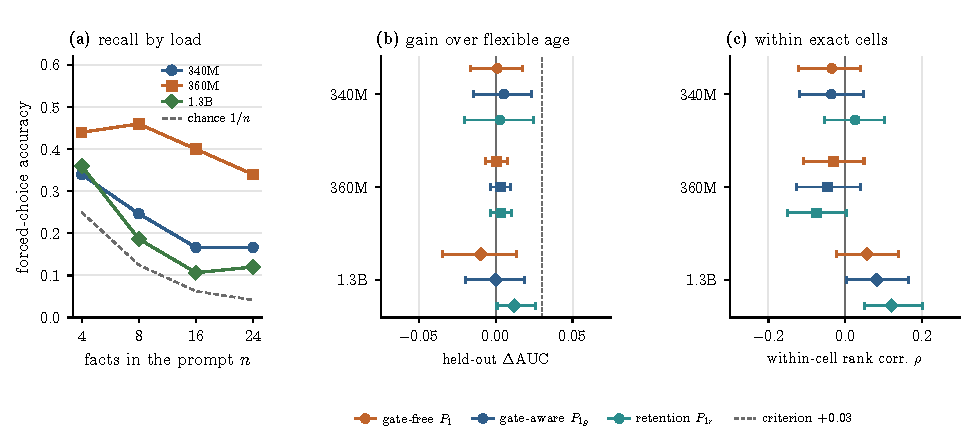
\includegraphics{fig_scale.pdf}
  \caption{The task-level test in three Gated DeltaNets (post hoc extension to 1.3B). (a) Forced-choice recall against load. (b) Held-out AUC gain over the flexible categorical-age baseline (95\% bootstrap intervals; the dashed line is the 0.03 criterion). (c) Rank correlation, within exact (load, queried position) cells, with the true value's log-probability among the candidates. Predictors: gate-free $P_1$, gate-aware $P_{1g}$ (interference, expected sign negative) and retention $P_{1r}$ (expected sign positive).}\label{fig:scale}
\end{figure}

\begin{table}[!htbp]
  \caption{Predictors of task-level recall in the 1.3B Gated DeltaNet (post hoc extension; 95\% bootstrap intervals), as in Table~\ref{tab:gatetask}. Twenty-four intervals in all, uncorrected.}\label{tab:scale}
  \centering\scriptsize\setlength{\tabcolsep}{3pt}
  \begin{tabular}{lccc}
\toprule
predictor & $\Delta$AUC, age + load & $\Delta$AUC, flexible age & within-cell $\rho$ \\
\midrule
$P_1$, gate-free $\psi$ (long-memory heads) & $-$.008 ($-$.029, $+$.011) & $-$.010 ($-$.034, $+$.013) & $+$.057 ($-$.023, $+$.139) \\
$P_{1g}$, gate-aware (long-memory heads) & $+$.003 ($-$.025, $+$.031) & $\pm$.000 ($-$.020, $+$.019) & $+$.082 ($+$.004, $+$.165) \\
$P_{1r}$, retention & $-$.001 ($-$.034, $+$.033) & $+$.012 ($+$.001, $+$.026) & $+$.121 ($+$.049, $+$.203) \\
decay only, $-\log A$ & $+$.015 ($-$.015, $+$.046) & $+$.023 ($-$.003, $+$.052) & $-$.032 ($-$.108, $+$.046) \\
$P_1$ shuffled within load & $+$.008 ($-$.017, $+$.032) & $+$.013 ($-$.027, $+$.050) & $-$.087 ($-$.168, $-$.008) \\
$P_{1g}$ shuffled within load & $+$.004 ($-$.013, $+$.021) & $+$.013 ($-$.021, $+$.045) & $-$.100 ($-$.177, $-$.029) \\
$P_{1b}$, gate-free, all heads & $-$.005 ($-$.031, $+$.018) & $-$.010 ($-$.029, $+$.007) & $\pm$.000 ($-$.080, $+$.083) \\
$P_{1g}$, all heads & $-$.007 ($-$.022, $+$.008) & $+$.015 ($-$.001, $+$.034) & $+$.085 ($+$.010, $+$.164) \\
\bottomrule
\end{tabular}

\end{table}

\textbf{Recall.} Forced-choice accuracy is \scAccFour, \scAccEight, \scAccSixteen\ and \scAccTwentyFour\ at $n=4,8,16,24$ (chance 0.25, 0.125, 0.06, 0.04; \scAccAll\ overall): above chance, but not stronger than in the 340M model (Figure~\ref{fig:scale}a). The larger model does not recall better in this format.

\textbf{Result.} The pre-registered-style gain of $P_1$ over age and one-hot load is $\scGfreeHD$ ($\scGfreeHLo$, $\scGfreeHHi$), and over the flexible age baseline $\scGfreeFlexD$ ($\scGfreeFlexLo$, $\scGfreeFlexHi$); for $P_{1g}$ the flexible-age gain is $\scGawareFlexD$ ($\scGawareFlexLo$, $\scGawareFlexHi$). The criterion (at least 0.03 with an interval excluding 0) is met by neither. Within exact cells the correlation of $P_1$ with the true value's log-probability is $\scGfreeInD$ ($\scGfreeInLo$, $\scGfreeInHi$); that of $P_{1g}$ is $\scGawareInD$ ($\scGawareInLo$, $\scGawareInHi$), an interval that narrowly excludes zero in the direction opposite to the hypothesis (higher interference, better recall). The shuffled controls, which share one permutation, give $\scGfreeshIn$ and $\scGawareshIn$ with intervals that exclude zero in the other direction, which shows how far a single within-cell estimate fluctuates in this model. The retention predictor $P_{1r}$, whose expected sign is positive, is the one association in the expected direction: a flexible-age gain of $\scGretFlexD$ ($\scGretFlexLo$, $\scGretFlexHi$) and a within-cell correlation of $\scGretInD$ ($\scGretInLo$, $\scGretInHi$), below the criterion. Six of the twenty-four intervals exclude zero, two of them the shuffled controls. By the verdict rule fixed in advance (a larger model ``confirms the null'' if neither $P_1$ nor $P_{1g}$ reaches the criterion and their within-cell intervals include zero) the outcome is \emph{mixed}, because the within-cell interval of $P_{1g}$ excludes zero; no predictor reaches the criterion.

\textbf{Reading.} The larger model leaves the picture of Section~\ref{sec:task} unchanged for the gate-free quantity, which carries no information beyond age and load. The gate-aware predictors show at most small associations whose sign is not consistent (the within-cell correlation of $P_{1g}$ is $\scGawareInD$ here against $\gWithinRa$ and $\gWithinRb$ in the two small models). Recall at this scale is as weak as in the small models, so the test has the same limited power; whether the key-only quantity predicts recall in models with stronger recall or in longer contexts remains untested.

%==============================================================================
\section{Systematic literature review}\label{app:review}
\subsection{Protocol and flow}
A protocol (research questions, sources, search strings, screening stages, eligibility criteria, coding, snowballing seeds and stopping rule) was written before any search. The sources were the arXiv API and the OpenAlex API (title-and-abstract search); not searched: Web of Science, Scopus, IEEE Xplore, ACM DL, Google Scholar, Semantic Scholar (rate-limited without a key), books, theses, non-English venues. Fourteen pre-specified search strings (S1--S14) covered continual learning in SSMs and linear-attention models (S1, S2), continual linear-regression theory (S3, S4), projection and null-space methods (S5), stability--plasticity theory (S6), memory and complexity results (S7, S13, S14), delta-rule and associative-memory capacity (S8, S9), adapters (S10), Grassmannian covering numbers (S11) and loss of plasticity (S12). \textbf{Amendment 1} (post hoc, after a recall check) added S15--S17 on delta-rule theory, task ordering and online-learner views of SSMs. \textbf{Amendment 2} (post hoc, after an end-to-end recall check) re-screened by title all 962 records that the Stage-1 keyword rule had discarded.

\begin{figure}[!htbp]
  \centering
  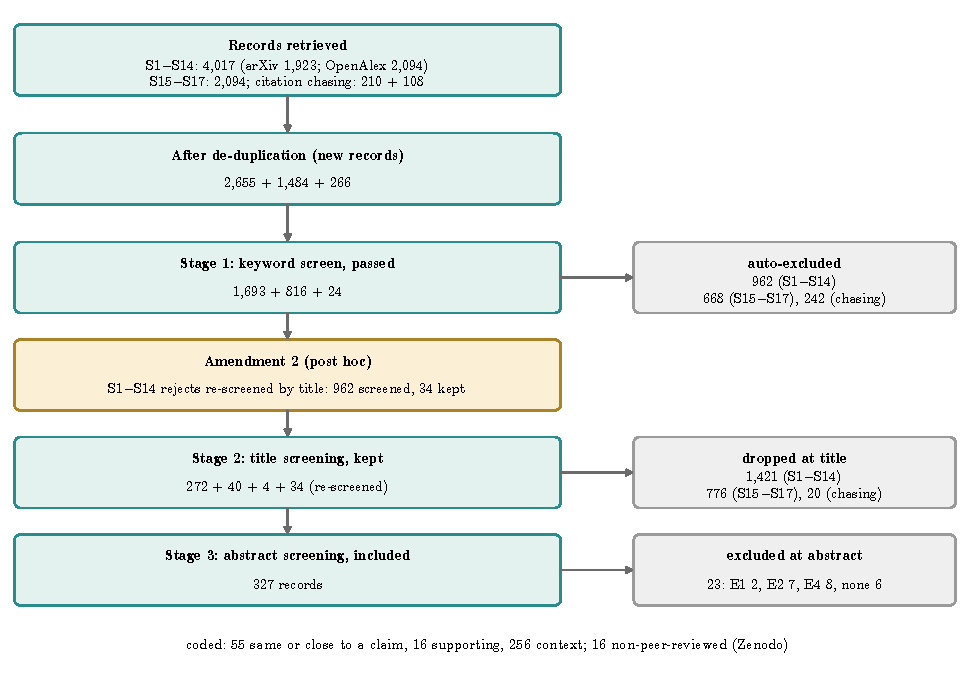
\includegraphics[width=\linewidth]{fig_prisma.pdf}
  \caption{PRISMA-style flow of the systematic literature search. The three counts joined by ``+'' are the pre-specified searches S1--S14, the supplementary searches S15--S17 and the citation chasing; the re-screening and the abstract-level step are post-hoc amendments.}\label{fig:prisma}
\end{figure}

\subsection{Recall checks}
Against 33 papers found earlier by ad hoc search: 27/33 retrieved by S1--S14 (82\%); 29/33 retrieved by S1--S17 (88\%); 23/33 after the Stage-1 keyword rule; 21/33 after title screening; \textbf{25/33 (76\%) end to end after Amendment 2}.
\begin{figure}[!htbp]
  \centering
  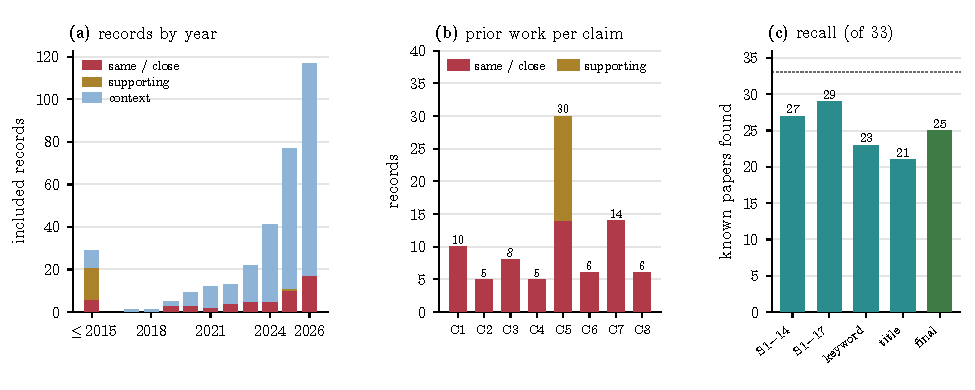
\includegraphics[width=\linewidth]{fig_review.pdf}
  \caption{The review. (a) Included records by year and overlap level. (b) The closest prior records per claim of the protocol. (c) Recall of the pipeline on a 33-paper reference set found by ad hoc search: the keyword rule lost six known papers, Amendment 2 recovered four.}\label{fig:review}
\end{figure}
Not included at the end: Jeong et al.\ (OpenAlex holds no abstract); InfLoRA and O-LoRA (retrieved, then classed as empirical adapter-family context); and five delta-rule / test-time-training architecture papers (Titans, Longhorn, DeltaNet, Gated DeltaNet, TTT), which are framed as sequence modelling, not continual learning. Recall is good for continual-learning theory and weaker for delta-rule architecture theory.

\subsection{Prior work found for each claim}
Table~\ref{tab:closest} lists, for each claim of the paper, the closest records found and how closely they overlap.
\begin{table}[!htbp]
  \caption{The closest records, by claim. ``Same'' = states essentially the same result; ``close'' = a special case, stronger/weaker form, or the same technique for a neighbouring setting. Evidence is the abstract unless stated; Zenodo = non-peer-reviewed.}\label{tab:closest}
  \centering\scriptsize\setlength{\tabcolsep}{3.5pt}
  \begin{tabular}{>{\raggedright\arraybackslash}p{1.25cm}>{\raggedright\arraybackslash}p{4.6cm}>{\raggedright\arraybackslash}p{1.8cm}>{\raggedright\arraybackslash}p{6.4cm}}
    \toprule
    claim & record & overlap & note \\
    \midrule
    delta-rule law & \textit{Attention as Conditioning} & close & DeltaNet's update is term-for-term Rescorla--Wagner error correction; exact closed form for blocking (cue competition) \\
    & \textit{Kaczmarz Linear Attention}~\citep{zou2026kaczmarz}; \textit{OSDN}~\citep{zhou2026osdn}; \textit{Fast Weight Attention for CL}~\citep{zhang2026fast} & close & derive delta-rule steps from the online-regression objective / Kaczmarz projection / NLMS; provable preconditioning \\
    & \textit{A Hippocampus for Linear Attention}~\citep{cui2026a} & close & caches the tokens with the largest $\beta\|e\|$, the committed residual (our ``surprise'') \\
    & Zenodo: \textit{Operator-Specific Forgetting in Matrix-Valued Associative Memory} & close & closed-form residual laws for selective forgetting; lineage theorem to the delta rule at $\beta{=}1$ \\
    capacity & Prados \& Kak~\citep{prados1989capacity}; 1989 dissertation & close (prior art) & storage capacity of the delta rule exceeds $N$ patterns in an $N$-neuron network \\
    & \textit{Anatomy of Associative Recall in Fixed-State Recurrences}~\citep{boesch2026anatomy}; \textit{How Linear Attention Remembers}~\citep{lee2026how}; \textit{On State Reduction in Linear Attention}~\citep{nazari2026on} & close & interference versus capacity in fixed-state recurrences; rank of the recurrent state shaped by keys and values \\
    no memoryless protector & Chen, Papadimitriou, Peng~\citep{chen2022memory}; Knoblauch et al.~\citep{knoblauch2020optimal} & close & memory growing linearly in tasks; optimal CL needs perfect memory \\
    minimal memory & \textit{ORFit} (Min, Cho, Azizan)~\citep{min2022orfit} & \textbf{same (construction)} & Lemma 3.1: projected-gradient step with step size set to interpolate leaves previous predictions unchanged; PCA truncation of the stored basis, claimed minimax \\
    & Dagan, Kur, Shamir~\citep{dagan2019space} & close (technique) & $\Omega(d^2)$ memory for streaming regression by a Grassmannian packing of $\exp(\Omega(d^2))$ subspaces \\
    & Dai, Liu, Rider~\citep{dai2007quantization}; Szarek; Pajor & close (covering) & quantisation / metric-entropy bounds on Grassmannians \\
    & \textit{Memory-Statistics Tradeoff in CL with Structural Regularization}~\citep{li2025memorystatistics} & close & memory (number of regularisation vectors) versus excess risk in two-task linear regression \\
    & Zenodo: \textit{The Stability-Plasticity Boundary} & close & $r(d-r)+r$-bit lower bound over $\mathbb F_2$ with a matching constructive learner \\
    & PMF-CL~\citep{nair2026pmfcl} (preprint) & close & what must be stored to minimise forgetting; Pareto-minimal learners for linear regression with $O(d^2)$ memory \\
    frontier & Zhao et al.~\citep{zhao2023rethinking}; AdaBOP; PMF-CL & close & stability/plasticity decoupling and adaptive orthogonal projection; Pareto analysis \\
    layerwise / SSM & GPM~\citep{saha2021gradient}; Adam-NSCL~\citep{wang2021training}; Mamba-CL~\citep{cheng2024mamba}; Inf-SSM~\citep{lee2025exemplar} & close & null-space projection of SSM parameters; observability-subspace regularisation \\
    forgetting theory & Evron et al.~\citep{evron2022catastrophic}; Levinstein et al.~\citep{levinstein2025optimal}; Lin et al.~\citep{lin2023theory} & close & rates and exact expressions for continual linear regression \\
    trace identity, calibrated bound & --- & none found & nearest: rank analyses of recurrent states; data-dependent forgetting bounds; no identity $n\,\mathrm{RMS}^2=\tr(MB)$, no value-free calibrated bound \\
    \bottomrule
  \end{tabular}
\end{table}

\subsection{Limitations of the review}
Two databases only; weak citation graphs for arXiv records in OpenAlex (the chasing returned 318 records and found no new close work); a single automated reviewer; abstract-level screening for most records (two papers read in full in the relevant sections, one record page); both amendments made after seeing results; end-to-end recall of 76\% on a reference set that was itself found by ad hoc search; 16 included records are non-peer-reviewed. This is a documented systematic search, not an exhaustive review.

%==============================================================================
\section{Verification, corrections and reproducibility}\label{app:verify}
\subsection{Validation of the re-implemented forward passes}\label{sec:val}
The Gated DeltaNet forward pass (\texttt{gdn\_extract.py}) was compared with an independent reference, the gated-delta-rule layer of the HuggingFace \texttt{transformers} library (the Qwen3-Next family: causal depthwise convolution with SiLU, $L_2$-normalised queries and keys, the gated delta rule with a chunked PyTorch kernel, and a gated RMS norm). The checkpoint's weights were mapped into that layer (\texttt{validate\_gdn\_reference.py}; no checkpoint code is executed and no kernel library is needed). The same hidden input is fed to both implementations at five layers, and in a second test the reference layer replaces ours in all layers of the full forward pass, on a 1024-token prose and a 1024-token code sequence per model.
\begin{table}[!htbp]
  \caption{Re-implementations against their references, float32. Gated DeltaNet: the \texttt{transformers} reference layer, 1024-token sequences; ``Layer'' is the largest relative output difference over the five checked layers, and the logit columns are for the full model with every attention layer replaced by the reference. RWKV-7: the NumPy reference in the authors' repository, run unmodified on the converted checkpoint, 512-token sequences; it exposes only the final logits.}\label{tab:validation}
  \centering\scriptsize\setlength{\tabcolsep}{3pt}
  \begin{tabular}{lccccccc}
\toprule
model & layer & max $|\Delta$logit$|$ & mean $|$logit$|$ & max KL & top-1 & prose ppl (ours / ref.) & code ppl (ours / ref.) \\
\midrule
Gated DeltaNet 340M & $6.1\times10^{-7}$ & $4.6\times10^{-5}$ & 3.8 / 3.2 & $4.7\times10^{-7}$ & 100\% & 7.4772 / 7.4772 & 3.6770 / 3.6770 \\
Gated DeltaNet 360M & $6.7\times10^{-6}$ & $1.7\times10^{-4}$ & 5.5 / 4.1 & $6.7\times10^{-7}$ & 100\% & 7.5987 / 7.5987 & 3.8146 / 3.8146 \\
Gated DeltaNet 1.3B & $4.3\times10^{-6}$ & $1.3\times10^{-3}$ & 17.2 / 16.0 & $5.9\times10^{-7}$ & 100\% & 5.8466 / 5.8466 & 3.0308 / 3.0308 \\
RWKV-7 0.1B & --- & $4.5\times10^{-5}$ & 17.3 / 21.0 & $3.0\times10^{-11}$ & 100\% & 7.5418 / 7.5418 & 3.1027 / 3.1027 \\
\bottomrule
\end{tabular}

\end{table}
The two implementations agree to float32 precision in every layer and in the logits, with identical top-1 predictions and perplexities. This validates our implementation of the recurrence, the convolution, the normalisations and the gating against an independent implementation of the same architecture; it does not compare against the original authors' \texttt{flash-linear-attention} kernels, which need a GPU (Triton) and were not run. Qwen3.5 and the two Transformers use library code. The same comparison was run for the 1.3B Gated DeltaNet of Appendix~\ref{app:scale}, whose checkpoint has no short convolution (the reference layer's convolution was set to an identity kernel, so that it computes SiLU of the projection): layer outputs agree to a relative $4.3\times10^{-6}$ and logits to $1.3\times10^{-3}$ at logit scale 16--17, with identical top-1 predictions and perplexity.

The RWKV-7 forward pass (\texttt{rwkv7\_flat.py}) was compared in the same spirit with the NumPy reference in the authors' repository (\texttt{rwkv\_v7\_numpy.py}, RWKV-v7 folder). Its functions were executed unmodified; only the part of that file that needs the original checkpoint, the \texttt{rwkv} package and hard-coded paths was not run. The cached checkpoint's tensors were mapped to the reference's parameter order (\texttt{validate\_rwkv7\_reference.py}), and both implementations were run token by token on 512 tokens of prose, code and project notes. In float64 the logits differ by at most $2.3\times10^{-13}$ (KL $<10^{-15}$); in float32, the precision the reference uses, by at most $4.5\times10^{-5}$ for logits of mean magnitude 14--21 (KL $<10^{-10}$), with identical top-1 predictions and perplexity (Table~\ref{tab:validation}). This validates the decay, the in-context learning rate, the removal and write keys, the value residual, the bonus term, the group norm and the token shifts, and the weight mapping, against independently written code. It does not compare against the authors' GPU kernels, and the reference file's own comparison with the \texttt{rwkv} package was not run.

\subsection{What was verified}
Every identity was checked on random instances to machine precision or to the stated tolerance. Each re-implemented forward pass (Gated DeltaNet 1 and 2, RWKV-7) was validated by perplexity and against an independent reference implementation (Section~\ref{sec:val}), and the RWKV-7 pass additionally by ablating components; Gated DeltaNet 1's recurrence was additionally checked against Lemma~\ref{lem:interf}. For Qwen3.5 the reconstruction from weights was compared with the library's captured keys and values. The algebra of Theorem~\ref{thm:surprise} (Kaczmarz step identity, minimum-norm interpolant, norm identity) and Proposition~\ref{prop:expq} (against an exact average over all permutations, $n=3,4,5$) were verified symbolically; the frontier theorem against independent solvers; the minimal-memory theorem numerically.

\subsection{What was not verified}
No re-implementation was compared against a reference \emph{output} from the original authors' kernels (none was available); the Gated DeltaNet re-implementations were compared with the \texttt{transformers} reference layer instead, and the RWKV-7 one with the NumPy reference in the authors' repository (whose decay constant, $e^{-1/2}$, it shares). Several references were checked at record or abstract level only.

\subsection{Reliability note}
Mixing torch and NumPy linear algebra in one process produced intermittent segmentation faults and non-finite values in our setup (each library alone was clean over thousands of repetitions), so the pipelines run torch (extraction, training) and NumPy (analysis) in separate processes. The single-process Gated-DeltaNet scripts never failed and satisfy the exact identities to $\lesssim10^{-14}$, but were not all rerun in the split configuration.

\subsection{Code and data}
\begin{sloppypar}
All code, the pre-registration, raw results and the review data are in the accompanying repository (\url{https://github.com/excyst-cerebral/delta-rule-key-geometry}): identities and bounds (\texttt{verify*.py}); model pipelines (\texttt{gdn\_*.py}, \texttt{qwen35\_flat.py}, \texttt{rwkv7\_flat.py}, \texttt{tf\_flat.py}); the training-time experiment (\texttt{exp\_mqar/}); the weight-space experiments (\texttt{exp\_cl/}, \texttt{exp\_mem/}, \texttt{exp\_bench/}); the task-level test (\texttt{exp\_task/}); and the review (\texttt{review/}). Checkpoints used (safetensors only; no repository code executed): \texttt{linear-moe-hub/Gated-Deltanet-340M} (799\,MB), \texttt{puigde/gated-deltanet-360M-15B-slimpajama} (1.43\,GB), \texttt{Qwen/Qwen3.5-0.8B-Base} (1.75\,GB), \texttt{fla-hub/rwkv7-0.1B-g1} (382\,MB, data files only), plus two locally cached Transformers; MNIST from the cvdf-datasets mirror (four files, 11.6\,MB).
\end{sloppypar}

%==============================================================================
\bigskip
\section*{Supplement: continual learning in the weights of small SSMs}
\addcontentsline{toc}{section}{Supplement: continual learning in the weights}
These results concern continual learning in the \emph{weights} of small SSMs and the question of whether forgetting in a pure SSM can be provably prevented without replay or anchoring. They share the algebra of Lemma~\ref{lem:interf} (forgetting is feature overlap times surprise) but concern a different setting from the context-state interference of the main text, so they are collected here: a summary (Appendix~\ref{app:weightsummary}), the theory (Appendix~\ref{app:weighttheory}) and the experimental details (Appendix~\ref{app:weightexp}). Most of the theory is known (ORFit/OGD, Grassmannian packing bounds, GPM-style projection; Section~\ref{sec:related}).

\section{Continual learning in the weights of small SSMs: summary}\label{app:weightsummary}
\textbf{Setting.} In the weights, the same identity holds: forgetting is feature overlap $\times$ surprise. For a learner linear in its features $\langle\theta,\phi(x)\rangle$ with old feature subspace $U$ (projector $P$, rank $r$), a new task $(\Phi,e)$ and update $\Delta$, define interference $\|P\Delta\|$ and fit error $\|\Phi\Delta-e\|$. With $G=\Phi(I-P)$ and $\Pi$ the projector onto its range:

\begin{theorem}[Protection--plasticity frontier]\label{thm:frontier}
(a) Zero interference is attained by $\Delta=G^{+}e$, with unavoidable fit error $\|(I-\Pi)e\|$; the targets fittable without interference lie in a space of dimension at most $\min(n,p-r)$. (b) The frontier $E^\ast(\varepsilon)=\min\{\|\Phi\Delta-e\|:\|P\Delta\|\le\varepsilon\}$ is traced by $\Delta_\mu=(\Phi^\top\Phi+\mu P)^{+}\Phi^\top e$, and $\mathrm{d}(E^{\ast2})/\mathrm{d}(\varepsilon^2)=-\mu$. (c) With one example of unit feature $w$, $\rho=\|Pw\|$, $\kappa=\|(I-P)w\|$ and a step budget $\|\Delta\|\le B$, zero interference leaves error $(|e|-\kappa B)_+$.
\end{theorem}
These statements were checked numerically against independent solvers (Figure~\ref{fig:frontier}). The zero-interference update in (a) is the ORFit/OGD update for linear models, and protecting an unknown $r$-dimensional subspace to interference $\delta'$ requires $r(p-r)\log_2(1/\delta')+O(r(p-r))$ bits by a Grassmannian packing argument; both are, in substance, known (Section~\ref{sec:related}; proofs in Appendix~\ref{app:weighttheory}).

\begin{figure}[!htbp]
  \centering
  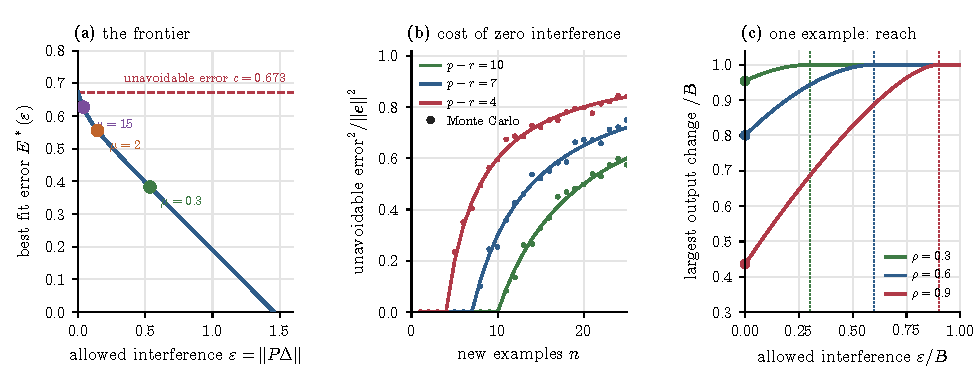
\includegraphics[width=\linewidth]{fig_frontier.pdf}
  \caption{The protection--plasticity frontier (Theorem~\ref{thm:frontier}); all curves computed from random instances. (a) A frontier ($p=12$, $r=5$, $n=10>p-r=7$ new examples, $\|e\|=1$): protecting the old subspace completely leaves \frontierPct\% of the new target's norm unfitted ($c=\frontierC$), and the fit improves only by accepting interference; the marked points are the solutions for three values of the multiplier $\mu$, and the slope of $E^{\ast2}$ against $\varepsilon^2$ at a point is $-\mu$. (b) The unavoidable error against the number of new examples, for three sizes of the protected subspace: the closed form $(n-\min(n,p-r))_+/n$ against Monte Carlo. (c) One new example with a step budget: allowing interference up to $\rho B$ recovers the full reach.}\label{fig:frontier}
\end{figure}

\textbf{Experiments.} All learners are plain SGD on small real-diagonal SSMs. \emph{Deep SSM on five synthetic conflicting tasks} (518 parameters, 5 seeds): fine-tuning forgets 0.63; gradient-subspace projection (storing 3--25 of 518 directions) leaves forgetting at 0.55--0.68, and the stored subspace had largely rotated by the end of the stream (mean squared cosine 0.15--0.35 with the same task's recomputed subspace); EWC reduces forgetting to 0.09--0.11 but the last task is learned only to 0.50--0.52; replay with 32 examples per task reaches final accuracy 0.88 with forgetting 0.12. A \emph{layerwise} scheme (project each linear layer's update off the stored subspace of its old input activations, recurrence frozen) is exact in the limit (Figure~\ref{fig:exact}) and gives forgetting 0.05--0.09 for under 7\,kbit, but the last task reaches only 0.31--0.63; with the recurrence free, or with poles never trained (a fixed random bank of time scales), protection or plasticity is not recovered.

\begin{table}[!htbp]
  \caption{Split-MNIST (5 tasks) and Permuted-MNIST (10 tasks) with a small SSM, 5 seeds. Final average accuracy (forgetting); the best learner without task identity in each column in bold. Joint training: 0.922 / 0.987 / 0.614. Layerwise = recurrence frozen, energy 0.99. Memory in bits (Split / Permuted). $^{\dagger}$ requires the task identity at test time and grows linearly with the number of tasks.}\label{tab:mnist}
  \centering\small\setlength{\tabcolsep}{4pt}
  \begin{tabular}{lcccc}
\toprule
Learner & bits (Split / Permuted) & Split, class-inc. & Split, task-inc. & Permuted \\
\midrule
Fine-tuning & 0 / 0 & .195 (.980) & .631 (.435) & .185 (.702) \\
EWC, $\lambda=10$ & 3.16\,M / 2.50\,M & .185 (.958) & .897 (.071) & .248 (.118) \\
Replay, 20 / task & 627\,600 / 1.26\,M & .605 (.461) & .932 (.061) & .315 (.532) \\
Replay, 200 / task & 6.28\,M / 12.6\,M & \textbf{.869} (.121) & \textbf{.980} (.007) & \textbf{.496} (.298) \\
Layerwise projection & 61\,453 / 92\,595 & .359 (.155) & .773 (.010) & .274 (.110) \\
Gradient subspace (OGD) & 11.4\,M / 67.2\,M & .195 (.979) & .689 (.362) & .210 (.697) \\
Task adapters (rank 4)$^{\dagger}$ & 195\,840 / 237\,888 & -- & .957 (.000) & .770 (.000) \\
\bottomrule
\end{tabular}

\end{table}

\begin{figure}[!htbp]
  \centering
  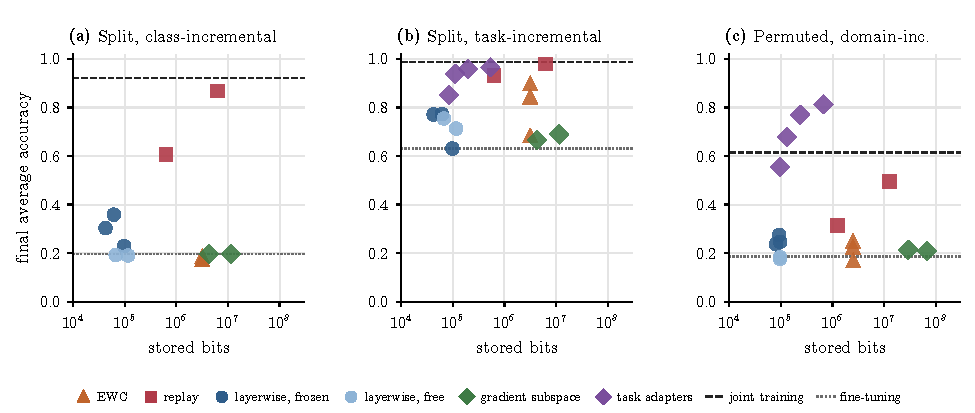
\includegraphics[width=\linewidth]{fig_mnist_pareto.pdf}
  \caption{Memory against accuracy on the three benchmarks (means over 5 seeds; dashed: joint training, dotted: fine-tuning). Adapters sit near the top-left but need the task identity in training and grow with the number of tasks; replay needs 5--30$\times$ more memory than adapters for similar accuracy; layerwise projection is cheap but plasticity-limited; gradient-subspace projection is dominated.}\label{fig:pareto}
\end{figure}

\textbf{Reading.} On a standard benchmark the picture repeats: replay is best in every setting, nothing without replay exceeds 0.36 class-incrementally, the frozen-recurrence layerwise scheme protects with 10--14$\times$ less memory than the smallest replay buffer but at a cost in plasticity, and gradient-subspace projection does not help. Per-task low-rank adapters and heads on a frozen backbone give exactly zero forgetting (old-task logits bit-for-bit unchanged) and high accuracy, at the price of memory that grows with the number of tasks and a task identifier: this leaves the premise of a pure fixed-size SSM. We did not reproduce the setting of published SSM continual-learning methods (a large pretrained vision Mamba on ImageNet-R and CIFAR-100); our models are small and the numbers are not comparable to theirs.

%==============================================================================
\section{Weight-space theory}\label{app:weighttheory}
\subsection{Weight-space interference}
Consider a model that is linear in features, $f(x;\theta)=\langle\theta,\phi(x)\rangle$ (the readout of any network, or the whole network to first order in the learning rate with $\phi=\nabla_\theta f$, the NTK feature map).
\begin{proposition}[Weight-space interference]\label{prop:wspace}
(1) One SGD step with step size $\eta$ on an example $(x',y')$ changes the prediction at any other input $x$ by $\Delta f(x)=-\eta\,\ell'(f(x'),y')\,\langle\phi(x),\phi(x')\rangle$, exactly, for any differentiable loss (for the squared loss $\ell'$ is the prediction error). This is Lemma~\ref{lem:interf} with $k\leftrightarrow\phi$, $\beta\leftrightarrow\eta$: \emph{forgetting $=$ feature overlap $\times$ surprise}.

(2) Let a new task $B$ with feature matrix $\Phi_B$ be interpolable and let gradient descent run to convergence from $\theta_0$. Then the old task's predictions change by $\Delta f_A=\Phi_A\Phi_B^{+}(y_B-\Phi_B\theta_0)$, the \emph{feature-overlap operator} $\Phi_A\Phi_B^{+}$ applied to the \emph{initial surprise} on the new task. It vanishes for every possible $y_B$ if and only if $\Phi_AP_B=0$, i.e.\ the old and new feature subspaces are orthogonal.

(3) If every channel's feature factorises as $z_c(x)=g_c(x)\psi_c(x)$ with gates $g_c\in[0,1]$ and $|\psi_c|\le\Psi$, and only the readout weights are trained, then $|\Delta f(x_{\mathrm{old}})|\le\eta\Psi^2\sum_s|\ell'_s|\sum_cg_c(x_{\mathrm{old}})g_c(x_s)$.
\end{proposition}
\begin{proof}
(1) $\nabla_\theta\ell=\ell'\phi(x')$. (2) The gradient steps stay in $\mathrm{row}(\Phi_B)$, and gradient descent from $\theta_0$ converges to the minimum-norm interpolating change $\Phi_B^{+}(y_B-\Phi_B\theta_0)$; $\Phi_A\Phi_B^{+}\Phi_B=\Phi_AP_B$, which vanishes for all $y_B$ in the range of $\Phi_B$ iff $\Phi_AP_B=0$. (3) Apply (1) and the triangle inequality to $\sum_cz_c(x_{\mathrm{old}})z_c(x_s)$.
\end{proof}
(Verified numerically: the identity to $4\times10^{-16}$; the closed form to the tolerance of finite gradient descent; orthogonal subspaces to $5\times10^{-14}$; the gate bound in 200 random trials.) Orthogonal-projection methods enforce $\Phi_AP_B=0$ by \emph{storing} a basis of $\mathrm{row}(\Phi_A)$; replay estimates $\Phi_A$ from stored examples; regularisation penalises movement in directions the stored Fisher says matter. In each case the object stored is exactly what part (2) says is needed.

\subsection{No pure learner can protect unknown old tasks}
\begin{theorem}[No memoryless guarantee]\label{thm:nomem}
Consider linear regression in $\R^2$, learner started at $\theta_0=0$. A new task $B$ has input $(1,0)$ and label $1$. There are two possible old tasks: $A_+$ (input $(1,1)/\sqrt2$, label 0) and $A_-$ (input $(1,-1)/\sqrt2$, label 0). $\theta_0$ fits both exactly and each is jointly realisable with $B$ ($\theta=(1,-1)$ for $A_+$, $(1,1)$ for $A_-$). Then any pure learner that fits $B$ to squared error $\le\epsilon$ ends at a point $\theta'$ with $\max(\mathrm{loss}_{A_+}(\theta'),\mathrm{loss}_{A_-}(\theta'))\ge(1-\sqrt\epsilon)^2/2$, whereas a learner that has stored one bit (which old task is active) reaches zero loss on both $B$ and the old task.
\end{theorem}
\begin{proof}
A pure learner's trajectory depends only on $\theta_0$ and the new-task examples, identical in the two scenarios, so it ends at the same $\theta'$ in both. Fitting $B$ forces $\theta'_1\ge1-\sqrt\epsilon$. The two old losses are $(\theta'_1\pm\theta'_2)^2/2$, whose sum is $\theta_1'^2+\theta_2'^2\ge\theta_1'^2$, so their maximum is at least $(1-\sqrt\epsilon)^2/2$.
\end{proof}
\begin{figure}[!htbp]
  \centering
  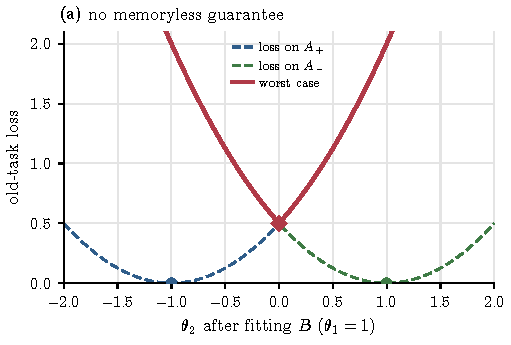
\includegraphics{fig_nomem.pdf}
  \caption{Theorem~\ref{thm:nomem}: the old-task losses after fitting task $B$ with $\theta_1=1$, as a function of $\theta_2$. Any pure learner lands at one $\theta_2$ for both possible old tasks and pays at least $\tfrac12$ on one of them; one stored bit reaches $\theta_2=\mp1$ and zero loss.}\label{fig:nomem}
\end{figure}

This is the elementary version of the statement that optimal continual learning requires memory \citep{knoblauch2020optimal}. It is \emph{not} a statement that learning cannot be organised so that most tasks do not interfere: Proposition~\ref{prop:wspace}(2) shows that when feature subspaces are orthogonal, nothing needs to be stored.

\subsection{What a selective SSM can and cannot offer}
In a selective SSM the state update of channel $c$ is multiplied by an input-dependent gate $\Delta_t^c=\mathrm{softplus}(w_c\cdot u_t+b_c)$. Since $g_c(x_{\mathrm{old}})\le1$, Proposition~\ref{prop:wspace}(3) implies a bound that uses only the new task's gates, $|\Delta f(x_{\mathrm{old}})|\le\eta\Psi^2\sum_s|\ell'_s|\sum_cg_c(x_s)$, which a learner can evaluate from the new data and the current parameters. It is a stability--plasticity statement: a new task that keeps most channels' gates closed cannot disturb much, whatever the old tasks are, but it also has little capacity to learn. The sharper bound shows protection when the \emph{old} inputs' gates avoid the channels the new task opens; that requires the gates to \emph{separate} the tasks, an assumption about the task stream (Theorem~\ref{thm:nomem}), and verifying it needs the old inputs' gates, so it is a certificate for an analyst, not for the learner. Routing by an observed task identifier into preallocated modules gives exactly zero interference at the price of parameters that grow with the number of tasks (Appendix~\ref{app:adapters}).

\subsection{How much must be stored? The minimal-memory theorem}
\textbf{Setting.} $f(x;\theta)=\langle\theta,\phi(x)\rangle$, $\theta\in\R^p$. The unknown old task has feature row-space $U\in\mathrm{Gr}(r,p)$ and is fitted exactly by the current $\theta_0$. A \emph{memory scheme} is any map $s:\mathrm{Gr}(r,p)\to\{0,1\}^m$ computed before the new task. The new task is one example with unit-norm feature $w$ and surprise $e$ (it needs $\langle w,\Delta\theta\rangle=e$), \emph{admissible} if it is jointly realisable with the old task with a margin, $\|(I-P_U)w\|\ge\kappa$, $\kappa\le1/\sqrt2$. Given $(s(U),w,e)$ the learner outputs $\Delta\theta=F(s(U),w,e)$ with $\langle w,\Delta\theta\rangle=e$. Its \emph{interference} is $\|P_U\Delta\theta\|/|e|$. Let $N(\varepsilon)$ be the covering number of $\mathrm{Gr}(r,p)$ in the metric $\|P-P'\|_{\mathrm{op}}=\sin\theta_{\max}$.

\begin{theorem}[Minimal memory for protection]\label{thm:minmem}
(a) \emph{Lower bound.} If a scheme guarantees interference $\le\delta'$ for every old task and every admissible $(w,e)$, then for $\delta'$ below a small absolute constant, $m\ge\log_2N(2\delta')\ge r(p-r)\log_2(c/(2\delta'))$. (b) \emph{Upper bound.} Storing the index of an $\varepsilon$-net point $\hat U$ ($m=\lceil\log_2N(\varepsilon)\rceil\le r(p-r)\log_2(C/\varepsilon)+1$ bits) and setting $\Delta\theta=e(I-P_{\hat U})w/\|(I-P_{\hat U})w\|^2$ fits the new example exactly and gives interference $\le\varepsilon/(\kappa-\varepsilon)^2$ for $\varepsilon<\kappa$. (c) Hence the minimal memory is $m^\ast(\delta')=r(p-r)\log_2(1/\delta')+O(r(p-r))$ bits: the metric entropy of the Grassmannian of the old feature subspace, i.e.\ its number of degrees of freedom times the log-precision.
\end{theorem}
Here $c,C$ are the absolute constants in the covering-number estimate $(c/\varepsilon)^{r(p-r)}\le N(\varepsilon)\le(C/\varepsilon)^{r(p-r)}$ for $\varepsilon$ up to a characteristic radius (Szarek; Pajor).
\begin{proof}
(a) Let $U_1,U_2$ share a message $s$, with largest principal angle $\theta$ and principal vectors $a_1\in U_1$, $a_2\in U_2$ ($\langle a_1,a_2\rangle=\cos\theta$). Put $w=(a_1-a_2)/\|a_1-a_2\|$, $\|a_1-a_2\|=2\sin(\theta/2)$. Then $\|(I-P_{U_1})w\|=\|(I-P_{U_2})w\|=\cos(\theta/2)\ge1/\sqrt2\ge\kappa$, so $w$ is admissible for both. The same $\Delta\theta$ must serve both, so $|e|=|\langle w,\Delta\theta\rangle|\le(\|P_{U_1}\Delta\theta\|+\|P_{U_2}\Delta\theta\|)/(2\sin(\theta/2))\le\delta'|e|/\sin(\theta/2)$, i.e.\ $\sin(\theta/2)\le\delta'$, hence $\sin\theta\le2\delta'$. Every message class therefore has diameter $\le2\delta'$ in the gap metric and lies in one ball of that radius, so $2^m\ge N(2\delta')$. (b) $\langle w,\Delta\theta\rangle=e$ by construction. With $\|P_U-P_{\hat U}\|\le\varepsilon$: $\|(I-P_{\hat U})w\|\ge\|(I-P_U)w\|-\varepsilon\ge\kappa-\varepsilon$, and $P_U(I-P_{\hat U})=P_U(P_U-P_{\hat U})$, so $\|P_U\Delta\theta\|/|e|\le\varepsilon/\|(I-P_{\hat U})w\|^2\le\varepsilon/(\kappa-\varepsilon)^2$. (c) Combine.
\end{proof}
\emph{Reading.} (i) The memory a pure-plus-memory learner needs depends on the dimension and precision of the old feature subspace, not on the number of old examples or tasks; replay stores $N\cdot p$ numbers and can be far larger. (ii) An explicit basis costs $r\cdot p$ numbers, a factor $p/(p-r)$ above the optimum. (iii) As $r\to p$ there is no room left: the stored object becomes cheap but the new task cannot be learned without disturbing the old one, so protection is paid for in plasticity (Theorem~\ref{thm:frontierfull}). (iv) Orthogonal-projection methods, and ORFit whose update is exactly the construction in (b), are the matching upper bound in this linear picture.

\textbf{Numerical checks.} The upper bound and exact fit hold to $10^{-14}$ with margin $1.3\times10^{-4}$; the pair construction holds to $7\times10^{-15}$ and the novelty component equals $\cos(\theta/2)$ to $4\times10^{-16}$; with a random codebook of $2^m$ subspaces the measured interference decays by a factor $2^{-0.490},2^{-0.256},2^{-0.168},2^{-0.112},2^{-0.085},2^{-0.149}$ per stored bit for $(r,p)=(1,3),(1,5),(2,5),(2,6),(3,6),(1,8)$ against the predicted $2^{-1/(r(p-r))}=2^{-0.500},2^{-0.250},2^{-0.167},2^{-0.125},2^{-0.111},2^{-0.143}$ (slightly shallower, as expected for a random rather than optimal codebook).

\begin{figure}[t]
  \centering
  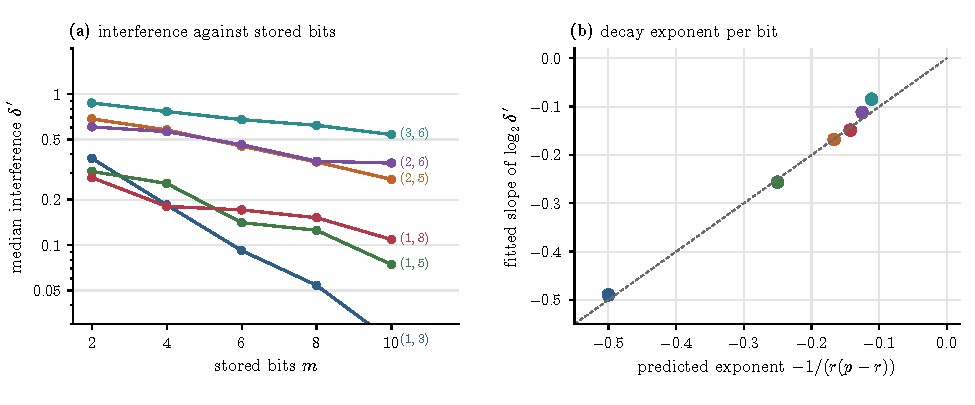
\includegraphics[width=\linewidth]{fig_minmem.pdf}
  \caption{Numerical checks of the minimal-memory theorem. (a) Median interference of the nearest of $2^m$ random codewords against the stored bits $m$ (solid) and the predicted slope $2^{-1/(r(p-r))}$ per bit anchored at the first point (dashed). (b) Fitted decay exponent against the predicted one; random codebooks are slightly shallower than the optimal codebook of the theorem, as expected.}\label{fig:minmem}
\end{figure}

\textbf{Provenance.} The construction in (b) is the ORFit/OGD update for linear models \citep{min2022orfit}; the counting argument in (a) is the Grassmannian-packing technique of \citet{dagan2019space}; covering numbers and quantisation bounds are classical \citep{szarek1998metric,pajor1998metric}. We did not re-derive the constants $c,C$ nor the admissible range of $\varepsilon$.

\subsection{The protection--plasticity frontier}\label{app:frontier}
Setting as in the main text: $\Phi\in\R^{n\times p}$, $e\in\R^n$, interference $I(\Delta)=\|P\Delta\|$, fit error $E(\Delta)=\|\Phi\Delta-e\|$, $G=\Phi(I-P)$, $\Pi$ the projector onto $\mathrm{range}(G)$, $c(e)=\|(I-\Pi)e\|$.
\begin{theorem}[Protection--plasticity frontier (full statement)]\label{thm:frontierfull}
(a) \emph{Zero forgetting.} $E^\ast(0)=c(e)$, attained by $\Delta=G^{+}e$. Since $\mathrm{rank}\,G\le\min(n,p-r)$, the targets fittable without interference form a subspace of dimension at most $\min(n,p-r)$; for $e\sim\mathcal N(0,\sigma^2I_n)$, $\E[c^2]=\sigma^2(n-\mathrm{rank}\,G)\ge\sigma^2(n-(p-r))_+$.
(b) \emph{The frontier.} $E^\ast$ is convex, non-increasing and $E^\ast(\varepsilon)\to c(e)$ as $\varepsilon\to0$. It is traced exactly by $\Delta_\mu=(\Phi^\top\Phi+\mu P)^{+}\Phi^\top e$, $\mu\in(0,\infty)$: the pair $(\|P\Delta_\mu\|,\|\Phi\Delta_\mu-e\|)$ is a frontier point, interference decreases and fit error increases with $\mu$, and the price of protection is $\mathrm d(E^{\ast2})/\mathrm d(\varepsilon^2)=-\mu$.
(c) \emph{One example with a step budget.} For a single example with unit feature $w$, $\rho=\|Pw\|$, $\kappa=\|(I-P)w\|$ and $\|\Delta\|\le B$, the largest reachable output change under interference $\le\varepsilon$ is $\rho\varepsilon+\kappa\sqrt{B^2-\varepsilon^2}$ for $\varepsilon\le\rho B$ and $B$ otherwise. With zero interference the error is $(|e|-\kappa B)_+$.
(d) \emph{Sequential capacity.} If $T$ tasks are protected with subspaces of dimensions $r_1,\dots,r_T$, the next task's targets that can be fitted at zero interference lie in a space of dimension at most $p-\dim(U_1+\dots+U_T)\ge p-\sum r_t$; at most $\lfloor p/r\rfloor$ tasks with $r$-dimensional subspaces can be protected exactly.
\end{theorem}
\begin{proof}
(a) $P\Delta=0$ means $\Delta=(I-P)\Delta$ and $\Phi\Delta=G\Delta$, and $\min\|G\Delta-e\|=\|(I-\Pi)e\|$ is attained at $G^{+}e\in\mathrm{range}(I-P)$. $\mathrm{rank}\,G\le\mathrm{rank}(I-P)=p-r$ and $\le n$. For isotropic $e$, $\E\|(I-\Pi)e\|^2=\sigma^2\tr(I-\Pi)=\sigma^2(n-\mathrm{rank}\,G)$.
(b) The problem $\min\|\Phi\Delta-e\|^2$ s.t.\ $\|P\Delta\|^2\le t$ is convex with value $V(t)$ convex and non-increasing in $t=\varepsilon^2$, and Slater's condition holds for $t>0$. The KKT conditions give $\Phi^\top(\Phi\Delta-e)+\mu P\Delta=0$ with multiplier $\mu=-V'(t)$; this is $(\Phi^\top\Phi+\mu P)\Delta=\Phi^\top e$, solvable because $\mathrm{range}(\Phi^\top)\subset\mathrm{range}(\Phi^\top\Phi+\mu P)$, and any two solutions differ by an element of $\ker\Phi\cap\ker P$, which changes neither $E$ nor $I$. Monotonicity in $\mu$ follows from convexity of $V$; $\mu\to\infty$ forces $P\Delta\to0$.
(c) $\langle w,\Delta\rangle=\langle(I-P)w,\Delta_\perp\rangle+\langle Pw,P\Delta\rangle\le\kappa\|\Delta_\perp\|+\rho a$ with $a=\|P\Delta\|\le\varepsilon$ and $a^2+\|\Delta_\perp\|^2\le B^2$; $\rho a+\kappa\sqrt{B^2-a^2}$ increases for $a<\rho B$ and is maximal ($=B$, using $\rho^2+\kappa^2=1$) at $a=\rho B$.
(d) The protected subspace after $T$ tasks is $U_1+\dots+U_T$, of dimension $\le\sum r_t$, and (a) applies to it.
\end{proof}
\textbf{Numerical check} (\texttt{verify\_frontier.py}). (a) Closed form against \texttt{lstsq} to $10^{-12}$ and against an independent gradient descent to $6\times10^{-10}$ (300\,000 iterations; at 20\,000 iterations the descent was still up to 0.35 away on ill-conditioned instances, a convergence artefact we found and fixed); Monte-Carlo $\E[c^2]=6.374$ against the formula $6.370$. (b) The parametric frontier agrees with an independent projected-gradient solver to $4\times10^{-14}$, the shadow-price identity holds to $10^{-7}$ (relative) and the frontier is monotone; the comparison has power (changing the interference budget by 10\% moves the independent optimum by about 0.1). (c) The reach formula matches a 4001-point maximisation to $7\times10^{-9}$ and random sampling never exceeds it.

\subsection{Layerwise exactness}
\begin{proposition}[Layerwise exactness]\label{prop:layer}
Consider a network built from linear layers $W_\ell$ (with biases), pointwise non-linearities and SSM blocks whose recurrence parameters are held fixed. If every update satisfies $\Delta W_\ell a=0$ for every old input activation $a$ seen by layer $\ell$ (computed with the old weights; bias handled by augmenting $a$ with a constant), then the outputs on all old inputs are unchanged exactly.
\end{proposition}
\begin{proof}
Induction over layers: the first layer sees the unchanged input, its output is unchanged, so the next layer sees unchanged activations, and so on; an SSM block with fixed parameters maps equal inputs to equal outputs.
\end{proof}
This is the argument of GPM-style activation-subspace methods. It does not cover SSM recurrence parameters (poles, $B$, $C$), which are not applied as outer products to activations; for them one needs the old \emph{tangent} subspace, a first-order object. The exactness holds in the limit of an activation subspace that captures all of the energy of the old activations, and approximately at a finite energy threshold (Figure~\ref{fig:exact}).

%==============================================================================
\section{Weight-space experiments: details}\label{app:weightexp}
\subsection{Anchor-free, anchor and replay learners on a small SSM}
\textbf{Testbed.} Four tasks with disjoint 16-token vocabularies; a task is ``is the signed sum of the tokens positive?'' with random $\pm1$ token signs, on length-15 sequences, learnt by a small SSM (24 channels $\times$ 4 states) with a \emph{shared} trainable SSM and readout. Token embeddings are \emph{fixed random} 16-dimensional vectors (otherwise disjoint vocabularies would never conflict), so 64 tokens share a 16-dimensional input space and interference is real. Two architectures: a diagonal LTI SSM and a Mamba-style selective SSM. Learners: fine-tuning (pure), EWC (anchor), replay (64 examples per old task), joint training (capacity reference), and two task-agnostic anchor-free regularisers on the selective gate (L1 sparsity, token-wise decorrelation of gate profiles). Five seeds; 400 steps per task; forgetting $=$ mean over old tasks of (best accuracy $-$ final accuracy).

\begin{table}[!htbp]
  \caption{Toy SSM testbed (5 seeds; mean $\pm$ s.d.). For the two regulariser settings the two numbers are for the two weights.}\label{tab:toy}
  \centering\scriptsize\setlength{\tabcolsep}{4pt}
  \begin{tabular}{llccc}
\toprule
arch & learner & final avg.\ accuracy & forgetting & paired $\Delta$ forgetting (wins) \\
\midrule
LTI & joint (reference) & .793$\pm$.072 & -- & -- \\
LTI & fine-tuning (pure) & .623$\pm$.059 & \textbf{.385$\pm$.077} & -- \\
LTI & EWC (anchor) & .686$\pm$.063 & .247$\pm$.066 & $-$.138 (5/5) \\
LTI & replay & .766$\pm$.076 & .138$\pm$.082 & $-$.247 (5/5) \\
selective & joint (reference) & .936$\pm$.043 & -- & -- \\
selective & fine-tuning (pure) & .687$\pm$.102 & \textbf{.368$\pm$.138} & -- \\
selective & + gate sparsity, $\lambda=0.01/0.03$ & .692/.685 & .354/.334 & $-$.014 (4/5) / $-$.033 (4/5) \\
selective & + gate decorrelation, $\lambda=0.5/2$ & .691/.709 & .363/.331 & $-$.005 (4/5) / $-$.036 (2/5) \\
selective & EWC (anchor) & .687$\pm$.136 & .252$\pm$.142 & $-$.115 (4/5) \\
selective & replay & .882$\pm$.046 & .076$\pm$.030 & $-$.292 (5/5) \\
\bottomrule
\end{tabular}

\end{table}

\begin{figure}[!htbp]
  \centering
  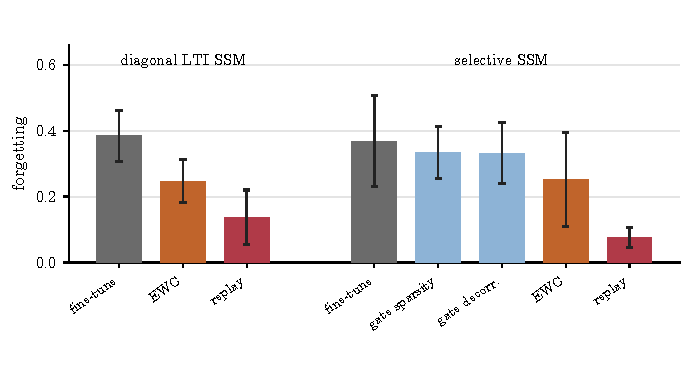
\includegraphics{fig_toy.pdf}
  \caption{Forgetting of each learner in the toy testbed (bars: mean; whiskers: $\pm1$ s.d. over five seeds). Task-agnostic gate regularisers (sparsity $\lambda=0.03$, decorrelation $\lambda=2$) are within noise of fine-tuning; learners that store information about the past help.}\label{fig:toy}
\end{figure}

\textbf{Findings.} (1) Pure learners forget substantially (0.37--0.39) in both architectures; the selective SSM has far more capacity (joint 0.94 against 0.79) but no more retention under plain fine-tuning. (2) Task-agnostic overlap-reducing regularisers are within noise ($-0.005$ to $-0.036$ against a between-seed spread of $\approx0.08$--0.14). (3) EWC removes about a third of the forgetting; replay two-thirds (LTI) to four-fifths (selective). (4) The gate-overlap proxy of Proposition~\ref{prop:wspace}(3) does not predict drops (Spearman $-0.02$ on 150 events; with the new task's initial loss $+0.30$): the gate profiles of different tasks were nearly parallel, so the proxy had no variation to explain.

\textbf{The weight-space law on the SSM's own features.} Training only a linear readout on the (random-initialised) SSM's final-state features, sequentially on two tasks (120 ordered task pairs across both architectures and five seeds), the realised change of the old predictions agrees with the first-step law with Spearman 0.98--1.00 (median ratio 2.0 between the change after 200 steps and the first-step prediction). The accuracy drop is explained by the new task's surprise (Spearman 0.57--0.65), not by the subspace overlap $\|\Phi_AP_B\|_F/\|\Phi_A\|_F$ (Spearman $\approx0$): with a 16-dimensional input every task's features span essentially the whole 24-dimensional feature space, so the overlap factor is saturated at $\approx1$. The identity is exact; the testbed simply lacks near-orthogonal task features.

\subsection{Memory against forgetting on the SSM's own features (readout only)}
Readout-only sequential learning on the final-state features ($p=24$ plus a bias) of the random-initialised SSMs, four tasks, ten (architecture $\times$ seed) runs, squared loss. The numerical rank of a task's standardised feature matrix is 24 at a 1\% singular-value tolerance and 16 (LTI) / 11 (selective) at 10\%, so old and new tasks fill most of the feature space.
\begin{table}[!htbp]
  \caption{Memory against forgetting, readout only.}
  \centering\scriptsize\setlength{\tabcolsep}{3.5pt}
  \resizebox{\linewidth}{!}{\begin{tabular}{>{\raggedright\arraybackslash}p{5.2cm}cccc}
    \toprule
    learner & bits stored & forgetting & last-task accuracy & final avg.\ accuracy \\
    \midrule
    fine-tuning & 0 & 0.289 & 0.787 & 0.559 \\
    projection, 8 bits/entry, energy 0.5/0.8/0.95/0.99 & 1240/2500/4340/5000 & 0.016/0.011/0.011/0.015 & 0.473/0.380/0.360/0.358 & 0.587/0.563/0.554/0.542 \\
    projection, energy 0.95, 4/2 bits per entry & 2050/695 & 0.029/0.127 & 0.374/0.651 & 0.553/0.570 \\
    EWC (stiff, one untuned weight) & 6400 & 0.004 & 0.502 & 0.572 \\
    replay, 8/64 examples per task & 25\,632/205\,056 & 0.159/0.156 & 0.737/0.733 & 0.617/0.626 \\
    \bottomrule
  \end{tabular}}
\end{table}
Stored projections of a few hundred to a few thousand bits remove 95\% of the forgetting, and quantisation to 2 bits per entry already costs protection (forgetting 0.127), as the precision term $\log_2(1/\delta')$ predicts. But zero forgetting is paid for in plasticity: the last task's accuracy falls from 0.79 to 0.36--0.47, and replay, which can compromise, has the best final average at 20--40 times the memory.

\subsection{Deep SSM on five conflicting tasks}
\textbf{Setup.} Each task is a length-48 noisy scalar sequence ($\mathcal N(0,0.1^2)$) with a $\pm1.5$ pulse a task-specific number of steps $d\in\{2,5,9,14,20\}$ before the end; the label is the pulse sign times a random task polarity, so tasks conflict through the shared kernel. Model: Linear(1$\to$12) $\to$ SSM $\to$ SiLU $\to$ Linear(12$\to$12) $\to$ SSM $\to$ last step $\to$ Linear(12$\to$2), real poles $\sigma(\mathrm{raw})$, state size 4, 518 parameters; plain SGD (lr 0.03, 600 steps per task, batch 64, gradient clipping at 5); five seeds, same data streams across learners. Gradient-subspace projection (OGD-style): after each task store a quantised basis of the per-sample logit-difference gradients (96 samples; energy $\rho$; $q$ bits per entry) and project later gradients off it.

\begin{table}[!htbp]
  \caption{Deep SSM, 5 seeds (first grid).}\label{tab:deep}
  \centering\scriptsize\setlength{\tabcolsep}{4pt}
  \resizebox{\linewidth}{!}{\begin{tabular}{>{\raggedright\arraybackslash}p{3.6cm}rcccc}
\toprule
learner & bits & final avg & forgetting & last task & $\Delta$forgetting (wins) \\
\midrule
fine-tuning & 0 & .49 & .633 & .997 & -- \\
projection, $\rho=0.5/0.9/0.99/0.9999$, 32 bits & 82\,880/112\,717/202\,227/411\,085 & .49/.47/.56/.50 & .634/.655/.547/.615 & .995/.987/.983/.990 & $+$.001/$+$.023/$-$.086/$-$.018 (3/3/4/4/5) \\
projection, $\rho=0.9$, 2/4/8 bits & 2\,901/14\,090/28\,179 & .48/.46/.46 & .653/.678/.668 & .994/.996/.987 & $+$.021/$+$.045/$+$.035 (3/2/3/5) \\
EWC, $\lambda=1/10/100$ & 165\,760/165\,760/165\,760 & .54/.53/.53 & .108/.096/.090 & .498/.521/.511 & $-$.525/$-$.537/$-$.542 (5/5/5/5) \\
replay, 4/32 per task & 30\,740/245\,920 & .80/.88 & .226/.122 & .973/.956 & $-$.407/$-$.511 (5/5/5) \\
\bottomrule
\end{tabular}
}
\end{table}

\begin{figure}[!htbp]
  \centering
  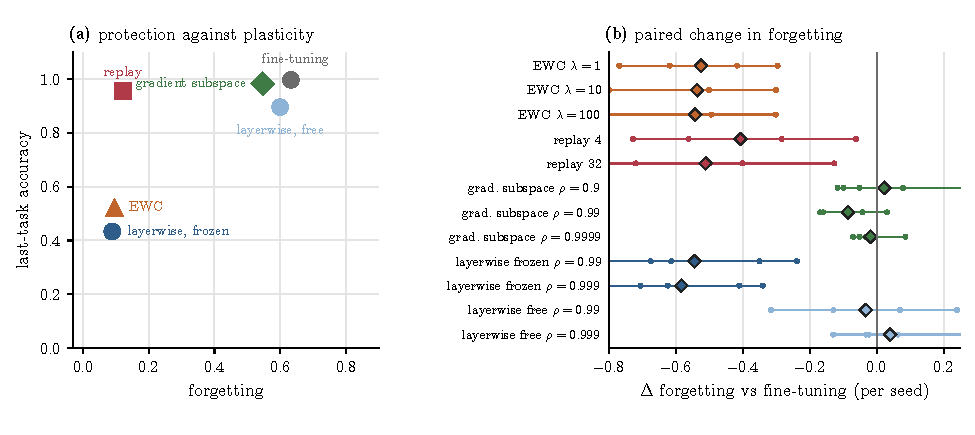
\includegraphics[width=\linewidth]{fig_deep1.pdf}
  \caption{The deep SSM on five conflicting tasks (5 seeds). (a) Forgetting against last-task accuracy for one representative setting of each learner (all settings and standard deviations are in the table): every learner that protects without replay loses the ability to learn the last task. (b) Paired change of forgetting relative to fine-tuning, per seed (dots) and mean (diamond).}\label{fig:deep1}
\end{figure}

\textbf{A candidate mechanism, measured once.} At the end of the stream we recomputed the gradient subspace of each old task on the final model ($\rho=0.99$) and compared it with the subspace stored when the task was learned. The mean squared cosine of the principal angles is $0.15,0.22,0.26,0.35$ for tasks learned $4,3,2,1$ tasks earlier, and the largest principal angle has $\sin\theta_{\max}=0.90$--$0.99$; a random 2--3-dimensional subspace of a 518-dimensional space would give about 0.005. The stored subspace is related to the later one but has largely rotated. This is consistent with the failure but does not prove it: the late subspace is computed on a model that has already forgotten the task, and each stored subspace had only 2--3 directions.
\begin{figure}[!htbp]
  \centering
  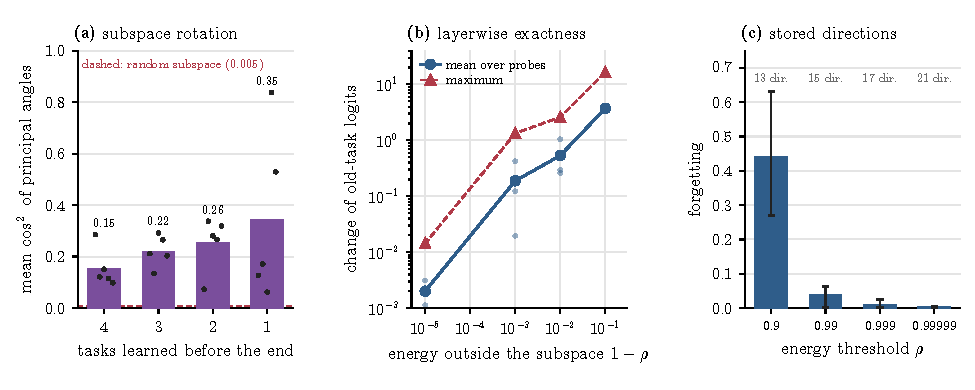
\includegraphics[width=\linewidth]{fig_deep3.pdf}
  \caption{Mechanisms in the deep SSM. (a) Rotation of the stored gradient subspace: mean squared cosine of the principal angles between the stored and the final-model subspace, per task (bars: mean of 5 seeds; dots: seeds) against a random subspace. (b) Exactness of layerwise protection with a frozen recurrence (3 seeds): the change of the old tasks' logits vanishes as the stored activation subspace captures all of the energy. (c) Forgetting and the number of stored directions at each energy threshold.}\label{fig:exact}
\end{figure}

\begin{figure}[!htbp]
  \centering
  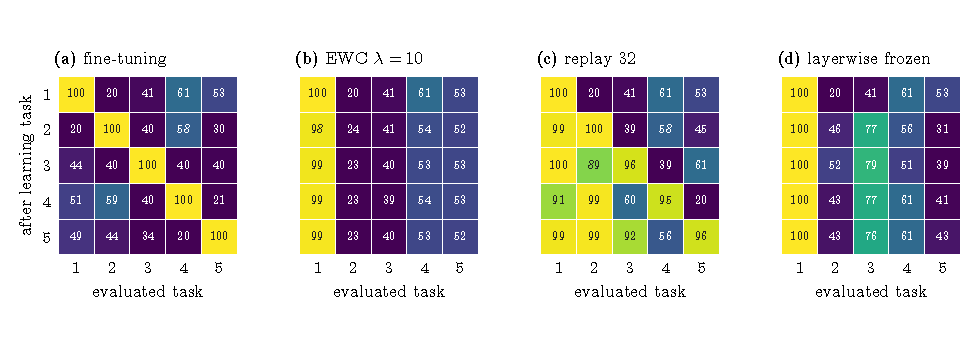
\includegraphics[width=\linewidth]{fig_deep2.pdf}
  \caption{Accuracy matrices of four deep-SSM learners (mean of 5 seeds): row $i$ shows the accuracy of each task after learning task $i$. Fine-tuning learns every task and forgets all earlier ones; EWC and layerwise protection retain the early tasks but learn the later ones poorly; replay does both best.}\label{fig:deepmat}
\end{figure}

\textbf{Layerwise activation-subspace protection.} For each linear layer (\texttt{Linear(1$\to$C)}, \texttt{Linear(C$\to$C)}, head) store a quantised basis of the span of its old input activations (all time steps of 256 sampled sequences per task, plus a constant column for the bias; energy threshold $\rho$) and project that layer's weight-and-bias gradient off it. Recurrence parameters are \emph{frozen} after task 0, \emph{free}, or \emph{gradient-projected} (a stored gradient subspace restricted to those coordinates).
\begin{table}[!htbp]
  \caption{Layerwise protection (5 seeds; $C=12$ unless stated).}
  \centering\scriptsize\setlength{\tabcolsep}{3.5pt}
  \begin{tabular}{>{\raggedright\arraybackslash}p{5.6cm}rccc}
    \toprule
    learner & bits & final avg & forgetting & last task \\
    \midrule
    recurrence \textbf{frozen}, $\rho=0.99/0.999$, 32 bits & 5286/6035 & .646/.608 & .089/.049 & .43/.31 \\
    same, $\rho=0.99$, 8/4 bits & 1321/692 & .657/.683 & .092/.201 & .49/.63 \\
    recurrence \textbf{free}, $\rho=0.99/0.999$ & 6118/7366 & .498/.460 & .600/.673 & .90/.99 \\
    recurrence \textbf{gradient-projected}, $\rho=0.99/0.999$ & 112k/154k & .472/.546 & .631/.544 & .89/.91 \\
    $C=32$: fine-tuning & 0 & .47 & .662 & .989 \\
    $C=32$, frozen, $\rho=0.99/0.999$ & 13\,433/15\,545 & .637/.652 & .248/.231 & .37/.51 \\
    $C=32$: EWC ($\lambda=10$) / replay (32 per task) & 645\,760/245\,920 & .518/.848 & .089/.171 & .57/.97 \\
    lr 0.005, 3600 steps: fine-tuning / gradient projection & 0/156k & .504/.506 & .618/.616 & .995/.995 \\
    \bottomrule
  \end{tabular}
\end{table}
\textbf{Exactness check} (frozen recurrence; 3 seeds). On fixed probe inputs the mean change of the old tasks' logits after later tasks (mean absolute logit $\approx3.4$) is $3.7,0.53,0.19,0.002$ for $\rho=0.9,0.99,0.999,0.99999$ (maximum change $16.3,2.6,1.3,0.014$), with $13,15,17,21$ stored directions in total and forgetting $0.44,0.040,0.012,0.003$ (Figure~\ref{fig:exact}). The change vanishes as $\rho\to1$, as the layerwise argument says, and is not exactly zero at finite $\rho$ because the activation subspace is estimated from a finite sample and truncated by energy.

\textbf{Controls.} A smaller learning rate with proportionally more steps changes nothing (fine-tuning 0.618, gradient projection 0.616): the failure of gradient-subspace projection is not a step-size artefact. (The lazy regime needs a different parameterisation and was not tested; a smaller learning rate at fixed total step size follows the same gradient-flow path and does not make training lazier.) Widening to $C=32$ did not improve the layerwise scheme.

\textbf{Poles fixed at initialisation.} Never training the poles (a fixed bank of random time scales) lets the exactness argument cover the whole network, but plasticity is not recovered.
\begin{table}[!htbp]
  \caption{Poles never trained (5 seeds). Toy stream and Split/Permuted-MNIST; final avg.\ accuracy, forgetting, last task.}
  \centering\scriptsize\setlength{\tabcolsep}{3.5pt}
  \begin{tabular}{>{\raggedright\arraybackslash}p{4.3cm}ccc}
    \toprule
    setting / learner & final avg & forgetting & last task \\
    \midrule
    toy $C{=}12$, fine-tuning & .485 & .631 & .966 \\
    toy $C{=}12$, layerwise $\rho=0.99/0.999$ & .604/.600 & .167/.120 & .341/.379 \\
    toy $C{=}32$, fine-tuning & .478 & .641 & .961 \\
    toy $C{=}32$, layerwise $\rho=0.99/0.999$ & .640/.631 & .219/.175 & .333/.518 \\
    Split class-inc., joint / fine-tuning & .873 / .195 & 0 / .963 & .812 / .971 \\
    Split class-inc., layerwise $\rho=0.95/0.99/0.999$ & .298/.343/.222 & .510/.120/.006 & .490/.089/.000 \\
    Split task-inc., joint / fine-tuning & .976 / .745 & 0 / .275 & .962 / .971 \\
    Split task-inc., layerwise $\rho=0.95/0.99/0.999$ & .748/.739/.630 & .099/.037/.001 & .734/.665/.502 \\
    Permuted, joint / fine-tuning & .550 / .209 & 0 / .619 & .529 / .768 \\
    Permuted, layerwise $\rho=0.95/0.99/0.999$ & .231/.257/.250 & .316/.089/.011 & .341/.171/.177 \\
    \bottomrule
  \end{tabular}
\end{table}
The loss of plasticity under exact protection is therefore not due to poles tuned to the first task; it is already present with fixed poles, and is consistent with the stored activation subspaces of the \emph{linear} layers filling up and with new tasks conflicting with old features (Theorem~\ref{thm:nomem}). Fixing the poles also lowers the joint-training reference (0.873 against 0.922 class-incrementally, 0.976 against 0.987 task-incrementally, 0.550 against 0.614 on Permuted).

\subsection{Split-MNIST and Permuted-MNIST: protocol and full grid}\label{app:mnist}
\textbf{Protocol.} Each $28\times28$ image is a sequence of 28 steps of 28 values. Model: Linear(28$\to C$) $\to$ SSM $\to$ SiLU $\to$ Linear($C\to C$) $\to$ SSM $\to$ last step $\to$ Linear($C\to10$) with real diagonal poles; $C=64$ ($p\approx9.9$k) for Split and 32 ($p\approx3.9$k) for Permuted. \textbf{Split-MNIST}: five two-class tasks trained with the full 10-way cross-entropy and no task identity, evaluated class-incrementally (argmax over all ten logits) and task-incrementally (argmax over the task's two classes). \textbf{Permuted-MNIST}: ten tasks with fixed pixel permutations, 20\,000 training images per task, domain-incremental (10-way, no task id). Plain SGD with momentum 0.9 reset per task (learning rate 0.03 and 4 epochs for Split; 0.1 and 3 for Permuted). The base-training settings were tuned on fine-tuning only, on seed 0 (also an evaluation seed), \emph{before} any comparison; a learning rate of 0.01 underfit badly (just-learned accuracy 0.35--0.56 on Permuted), so 0.03 (Split) and 0.1 (Permuted) were used. All other hyper-parameters are reported as a full grid with no per-method selection. Memory is counted in bits: replay stores 8-bit pixels and a 4-bit label per example, EWC two float32 copies of the parameters per task, projection learners 32-bit basis entries. Five seeds throughout.

\begin{table}[!htbp]
  \caption{Split-MNIST, \emph{class-incremental}: final average accuracy, forgetting, last-task accuracy, bits (mean $\pm$ s.d.\ over 5 seeds; settings separated by slashes).}\label{tab:mnistci}
  \centering\scriptsize\setlength{\tabcolsep}{4pt}
  \resizebox{\linewidth}{!}{\begin{tabular}{lcccc}
\toprule
learner & final avg & forgetting & last task & bits \\
\midrule
fine-tuning & .195$\pm$.001 & .980$\pm$.003 & .976$\pm$.005 & 0 \\
EWC $\lambda=10/100/1000$ & .185/.172/.171 & .958/.861/.363 & .921/.778/.057 & 3.16\,M \\
layerwise, free, $\rho=0.95/0.99$ & .192/.190 & .966/.960 & .958/.950 & 66\,976/115\,949 \\
layerwise, frozen, $\rho=0.95/0.99/0.999$ & .303/.359/.229 & .581/.155/.001 & .511/.112/.000 & 42\,432/61\,453/97\,760 \\
OGD $\rho=0.9/0.99$ & .195/.195 & .978/.979 & .974/.976 & 4.29\,M/11.4\,M \\
replay $k=20/200$ & .605/.869 & .461/.121 & .962/.947 & 627\,600/6.28\,M \\
joint training & \multicolumn{4}{c}{.922$\pm$.007} \\
\bottomrule
\end{tabular}
}
\end{table}
\begin{table}[!htbp]
  \caption{Split-MNIST, \emph{task-incremental} (task id given at test time).}\label{tab:mnistti}
  \centering\scriptsize\setlength{\tabcolsep}{4pt}
  \resizebox{\linewidth}{!}{\begin{tabular}{lcccc}
\toprule
learner & final avg & forgetting & last task & bits \\
\midrule
fine-tuning & .631$\pm$.043 & .435$\pm$.056 & .976$\pm$.005 & 0 \\
EWC $\lambda=10/100/1000$ & .897/.842/.682 & .071/.032/.023 & .921/.791/.540 & 3.16\,M \\
layerwise, free, $\rho=0.95/0.99$ & .755/.713 & .262/.306 & .958/.950 & 66\,976/115\,949 \\
layerwise, frozen, $\rho=0.95/0.99/0.999$ & .771/.773/.631 & .093/.010/.000 & .734/.604/.537 & 42\,432/61\,453/97\,760 \\
OGD $\rho=0.9/0.99$ & .665/.689 & .390/.362 & .974/.976 & 4.29\,M/11.4\,M \\
replay $k=20/200$ & .932/.980 & .061/.007 & .976/.982 & 627\,600/6.28\,M \\
joint training & \multicolumn{4}{c}{.987$\pm$.002} \\
\bottomrule
\end{tabular}
}
\end{table}
\begin{table}[!htbp]
  \caption{Permuted-MNIST, domain-incremental (no task id).}\label{tab:mnistperm}
  \centering\scriptsize\setlength{\tabcolsep}{4pt}
  \resizebox{\linewidth}{!}{\begin{tabular}{lcccc}
\toprule
learner & final avg & forgetting & last task & bits \\
\midrule
fine-tuning & .185$\pm$.006 & .702$\pm$.007 & .810$\pm$.006 & 0 \\
EWC $\lambda=10/100/1000$ & .248/.223/.168 & .118/.032/.050 & .177/.192/.111 & 2.50\,M \\
layerwise, free, $\rho=0.95/0.99$ & .177/.183 & .569/.505 & .580/.554 & 95\,763/96\,608 \\
layerwise, frozen, $\rho=0.95/0.99/0.999$ & .236/.274/.247 & .370/.110/.017 & .353/.176/.150 & 80\,557/92\,595/96\,608 \\
OGD $\rho=0.9/0.99$ & .214/.210 & .687/.697 & .834/.831 & 29.3\,M/67.2\,M \\
replay $k=20/200$ & .315/.496 & .532/.298 & .752/.726 & 1.26\,M/12.6\,M \\
joint training & \multicolumn{4}{c}{.614$\pm$.009} \\
\bottomrule
\end{tabular}
}
\end{table}

\begin{figure}[!htbp]
  \centering
  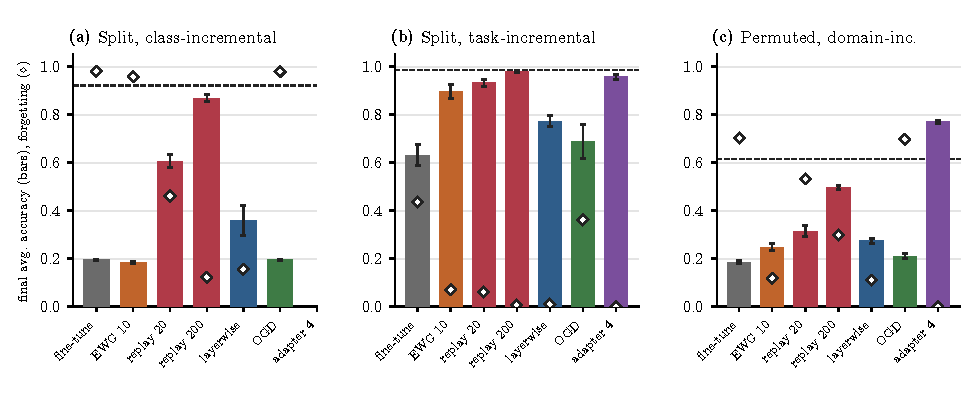
\includegraphics[width=\linewidth]{fig_mnist_bars.pdf}
  \caption{Final average accuracy (bars, $\pm1$ s.d.) and forgetting (diamonds) on the three benchmarks; dashed: joint-training references (0.922, 0.987, 0.614). Replay is best in every setting; without replay nothing exceeds 0.36 class-incrementally. Adapters need the task identity, so they have no class-incremental bar.}\label{fig:mnistbars}
\end{figure}

\begin{figure}[!htbp]
  \centering
  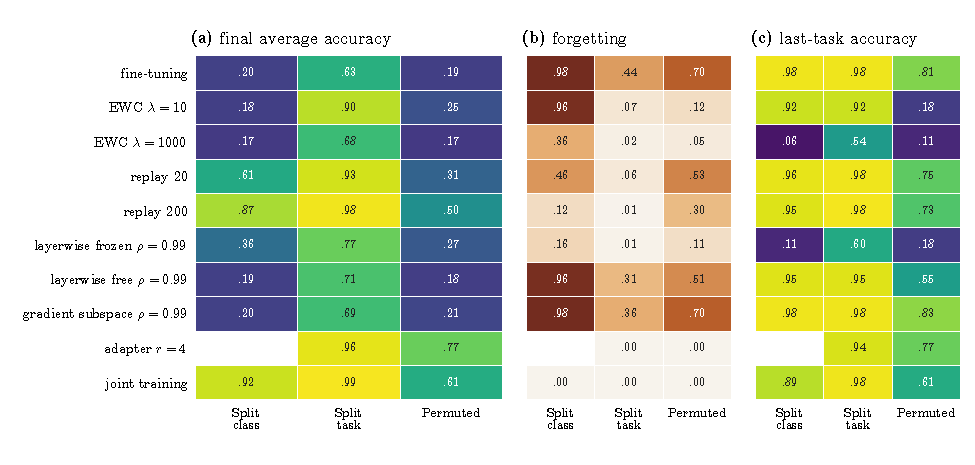
\includegraphics[width=\linewidth]{fig_mnist_heat.pdf}
  \caption{The benchmark grid as annotated heatmaps: final average accuracy, forgetting and last-task accuracy (blank: not applicable).}\label{fig:mnistheat}
\end{figure}

\begin{figure}[!htbp]
  \centering
  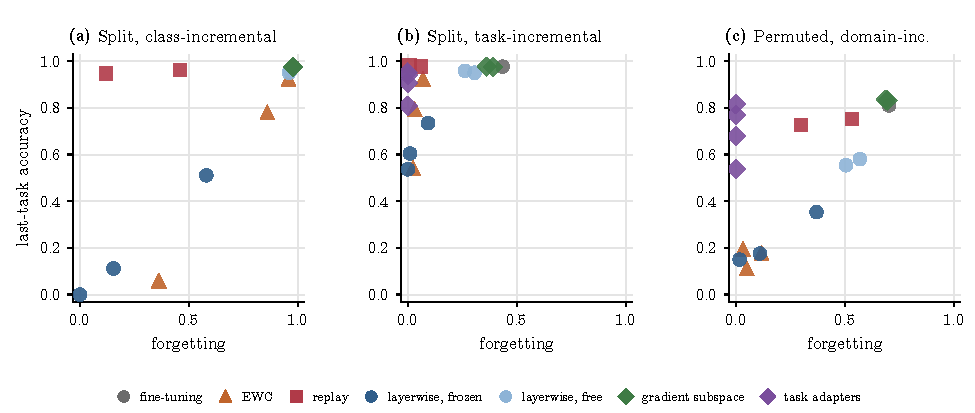
\includegraphics[width=\linewidth]{fig_mnist_plane.pdf}
  \caption{The stability--plasticity plane on the three benchmarks forgetting against last-task accuracy. Learners that protect lose plasticity; replay and adapters come closest to the ideal top-left corner.}\label{fig:mnistplane}
\end{figure}

\subsection{Task-specific adapters}\label{app:adapters}
Task 0 trains the whole network. For every later task the backbone, including the recurrence, is frozen and the task trains only its own output head and a rank-$r$ low-rank adapter on Linear(28$\to C$) and Linear($C\to C$) ($r=0$: head only). \textbf{The task identifier is used in training and at test time}, which none of the class- or domain-incremental learners receive; the comparison with them is fair only on Split-MNIST task-incrementally, where the other learners are also given the task identity at test time (by masking). Forgetting is exactly zero by construction and we verified it: the logits of an old task are bit-for-bit unchanged after later tasks (maximum change 0.0 in all 40 runs).
\begin{table}[!htbp]
  \caption{Task-specific adapters, 5 seeds; zero forgetting by construction.}\label{tab:adapters}
  \centering\small\setlength{\tabcolsep}{4pt}
  \begin{tabular}{lccc}
\toprule
learner & bits (Split / Permuted) & Split task-inc.\ acc & Permuted (task id) acc \\
\midrule
head only ($r=0$) & 83\,200 / 95\,040 & .852 & .554 \\
rank 1 + head & 111\,360 / 130\,752 & .939 & .677 \\
rank 4 + head & 195\,840 / 237\,888 & .957 & .770 \\
rank 16 + head & 533\,760 / 666\,432 & .965 & .814 \\
\bottomrule
\end{tabular}

\end{table}
\begin{figure}[!htbp]
  \centering
  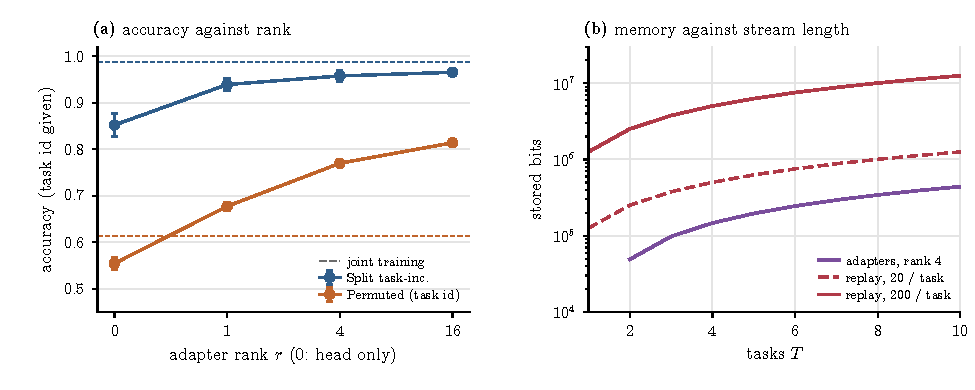
\includegraphics[width=\linewidth]{fig_adapters.pdf}
  \caption{Task-specific adapters. (a) Accuracy against adapter rank (bars: $\pm1$ s.d.; dashed: joint training). (b) Stored bits against the number of tasks: adapters and replay grow linearly.}\label{fig:adapters}
\end{figure}
Per-task memory grows linearly (about 49\,kbit per task for rank 4 on Split, 26\,kbit on Permuted), as the memory lower bound for general continual learners requires \citep{chen2022memory}, and a task identifier is needed at test time; class-incrementally, with no identifier, this learner is not applicable. In the terms of the definitions it is a pure learner on each task but an anchor-free \emph{architecture growth} on the stream, which our definitions did not classify and which we do not count as solving the original question.


\end{document}
